\documentclass{xdupgthesis}
\usepackage{tabularx}
\usepackage{subcaption}

\usepackage{tcolorbox}
\newtcolorbox{casebox}[2][]{colback=gray!5!white, colframe=black!75!black, title=#2, #1}
%\usepackage{xdufont}
\xdusetup{
	style = { 
		cjk-font = win, 
		latin-font = tac,
		ref-add-space=true, 
  		bib-backend=bibtex,
		add-alg-rule-vspace=false,
	},
	info = {
		%% 信息页 %%
		title = {西安电子科技大学研究生学位论文\\
		基于大语言模型思维链的文档摘要生成算法研究}, % 论文题目
		title* = {Research on Document Summarization Algorithm Based on Large Language Model Chain-of-Thought},
		author = {周佳和}, % 姓名
		author* = {Zhou Jiahe},
		supervisor = {苗启广},
		supervisor* = {Miao Qiguang},
		supv-title = {教授},
		supv-title* = {Professor},
		degree = {工学硕士},
		student-id = {23031212224},
		department = {广州研究院},
		clc = {TN82},
		major = {计算机科学与技术},
		major* = {Computer Science and Technology},
		sub-major = {计算机应用技术},
		submit-date = {2026-3},
		%% 摘要 %%
		abstract = {chapters/abstract-zh.tex}, % 摘要文件路径
		keywords = {文本摘要,大语言模型,思维链,检索增强生成},
        abstract* = {chapters/abstract-en.tex}, % 摘要文件路径
		keywords* = {Text Summarization,Large Language Models,Chain-of-Thought,Retrieval-Augmented Generation}, % 关键字
        % 符号对照表
        los = {chapters/los.tex},
        % 缩略语对照表
        loa = {chapters/loa.tex},
		%作者简介路径
		bio={chapters/bio.tex},
		%bib文件
		bib-resource={myref},
	}
}

\usepackage{amsmath}
\usepackage{amssymb} 
% \usepackage{subfig}
\usepackage{graphicx}
\usepackage{enumerate}
\usepackage{algorithm}
%\usepackage{algorithmic}
\usepackage{algorithmicx}
\usepackage{threeparttable}
\usepackage{algpseudocode}
\usepackage{multirow}
\usepackage{booktabs}
\usepackage{xcolor}

\usepackage{longtable} 
\usepackage{ulem}     % 提供 \uline
\usepackage{makecell}
% \usepackage[ruled,linesnumbered]{algorithm2e}
\usepackage{bm}

\begin{document}
\chapter{绪论}
本章旨在阐述基于多粒度主题感知与大模型协同的文本摘要算法的研究背景。首先,系统梳理自动摘要技术从统计机器学、预训练模型到大语言模型时代的演进脉络与实际应用价值。在此基础上,深入剖析当前文档摘要任务中面临的语义稀释、位置偏差及生成幻觉等核心挑战,为本文提出的研究思路奠定理论基础。

\section{研究背景及意义}

长期以来,阅读一直是人类获取知识与传承文明的核心途径。然而,随着移动互联网、物联网及数字化办公技术的全面普及,全球数据总量呈现出指数级增长趋势。在这一浩瀚的数据海洋中,以学术文献、行业研报、新闻资讯及法律案卷为代表的长文档占据了核心地位。面对海量数据的爆发性增长,文本信息的冗余性、无序性与人类有限的认知处理能力之间形成了供需矛盾,导致信息过载与获取低效并存的困境日益凸显。这一现象已成为制约科研学习、商业决策优化及办公效率提升的关键瓶颈。

因此,如何在海量文本中快速、准确地提炼核心内容,实现从数据到知识的高效转化,是当前人工智能与自然语言处理(Natural Language Processing,NLP)领域亟待解决的首要任务。在此背景下,自动文本摘要技术(Automatic Text Summarization, ATS)作为解决信息过载的核心手段,备受学术界与工业界的广泛关注。该技术旨在利用计算模型对冗长的源文档进行自动化的语义压缩与重构,生成简洁、连贯且保留核心语义的摘要,对于显著降低认知负荷、提升信息检索与理解效率具有重要的理论意义与应用价值。
\begin{figure}[H]
	\centering
	\label{fig:paperline}  
	\includegraphics[width=0.9\textwidth]{figure/chapter1/c0f0.pdf}
    \caption{摘要生成示意}
\end{figure}

纵观自动文本摘要技术的发展历程,其研究范式经历了由浅层特征统计向深层语义理解的演进。早期的摘要研究主要集中在抽取式摘要(Extractive Summarization)。这一阶段的方法依赖于人工设计的浅层特征,如词频(TF-IDF)、句子位置、标题重合度以及线索词等。最具代表性的是基于图排序算法的 TextRank 和 LexRank,它们将文档建模为句子网络,通过计算节点的中心度来筛选关键句。尽管这些方法具有无监督、计算效率高的优势,但由于缺乏对文本深层语义和篇章结构的理解,生成的摘要往往面临语义离散、连贯性差以及指代不明等问题。

随着深度神经网络的兴起,生成式摘要(Abstractive Summarization)迎来了突破性进展。基于循环神经网络(RNN)及其变体(LSTM\cite{yu2019review}, GRU\cite{cho2014learning})的序列到序列(Sequence-to-Sequence\cite{sutskever2014sequence}, Seq2Seq)框架成为主流。该框架通过编码器(Encoder)将源文本映射为连续的语义向量,再由解码器(Decoder)逐步生成目标摘要序列。特别是注意力机制(Attention Mechanism)\cite{bahdanau2014neural}的引入,有效缓解了长文本中的信息瓶颈问题,使得模型能够动态关注原文的不同部分。然而,RNN 架构固有的串行计算特性限制了并行训练能力,且难以捕捉长距离的语义依赖,导致生成的摘要容易出现重复、事实错误、集外词(OOV)无法识别及细节丢失等缺陷。

近年来,以 Transformer\cite{vaswani2017attention} 架构为基础的预训练语言模型(Pre-trained Language Models, PLMs)的横空出世,彻底重塑了 NLP 领域的技术格局,得益于其强大的上下文感知能力与多头注意力机制(Multi-Head Attention)的并行计算优势,预训练模型显著提升了文本的语义表征质量,为生成高流畅度、高语义覆盖度的摘要提供了坚实的技术底座。然而,尽管技术手段不断迭代,在处理复杂长文档时,现有的单一模型架构无论是基于BERT\cite{devlin2019bert}的抽取式模型,还是基于 大语言模型(Large Language Models, LLMs的生成式模型,仍难以同时兼顾覆盖度、准确度与流畅度。综上所述,需要能从人类阅读的角度出发,提出一种可读性更高的摘要生成算法。


\section{研究面临的挑战}
尽管基于深度学习的文本摘要技术已取得显著进展,但在处理长篇幅、多主题、高噪声的非结构化文档时,现有的主流方法仍面临诸多难以逾越的核心挑战。这些挑战主要集中在信息筛选的精准度、生成内容的可信度以及不同范式间的协同性三个维度。本文将这些挑战归纳为以下三个方面:

1.长文档编码中的语义稀释与位置偏差,在抽取式摘要任务中,从源文档中筛选出最具代表性的句子本质上是一个多目标优化的 NP-难问题,需要在最大化信息覆盖与最小化冗余之间寻求平衡。然而,在处理学术论文或行业研报等长文档时,基于 Transformer 的编码器面临着严峻的结构性缺陷。首先是语义稀释问题。标准自注意力机制在处理长序列时,注意力分布往往趋于发散。随着序列长度的增加,简单的关键词匹配无法捕捉隐含的核心语义,关键信息容易被淹没在海量的背景噪声中,导致模型难以在远距离的 Token 之间建立有效的强连接,从而遗漏低频但关键的论点。其次是位置偏差(Lead-3 现象)。由于预训练数据的分布特性及输入长度限制,现有模型往往过度依赖位置特征,倾向于抽取文档开头的句子。这种对局部细节或近期输入的过度聚焦,使得模型忽略了分布在文档中后部或跨段落的关键主题信息。如何引导模型突破局部视野的限制,是提升长文档抽取质量的首要难题。

2.生成式模型的幻觉风险与上下文限制,虽然生成式摘要通过模拟人类的认知重构过程,在文本流畅度上表现优异,但在长文档摘要任务中存在两大瓶颈。一方面是事实一致性缺失与幻觉风险。生成式模型本质上是基于概率分布预测下一个词,而非基于严格的逻辑推理。其核心难点在于如何在巨大的词汇组合空间中,精确平衡忠实度与流畅度。在缺乏强约束的情况下,模型极易生成语法正确但在语义上与源文档相悖的内容,这种幻觉现象严重损害了摘要在科研与商业决策中的可信度。另一方面是上下文窗口与迷失中间的问题。尽管 LLM 的上下文窗口在不断扩大,但直接输入超长文档不仅带来巨大的计算开销,还容易导致模型忽略中间部分的关键信息。随着序列长度增加,编码器会出现语义遗忘,难以维持对全局上下文的有效感知。如何构建高效的证据筛选机制,将长文档变薄后再输入生成模型,是实现高效且可信生成的关键。

3.抽取式与生成式方法的割裂与协同困境,当前学术界的研究往往将抽取式与生成式方法割裂看待,两者各有优劣且难以互补。抽取式方法虽然忠实于原文,但其从原文不同位置剥离句子的做法切断了上下文联系。这导致生成的摘要缺乏必要的逻辑连接词和过渡语,读起来突兀、跳跃,且常出现指代不明(如代词“他”、“这”指代对象缺失)的问题,造成理解障碍。反观生成式方法,虽然解决了语义融合与句法重组的问题,提升了可读性,但其黑盒特性使得内容难以溯源,且容易陷入语言退化或重复生成的局部最优循环。因此,如何融合两者的优势,构建一种抽取-生成协同进化的新范式,既利用抽取模型精准定位关键事实并解决长文档的语义稀释问题,又利用生成模型进行逻辑重构与润色以解决碎片化问题,并引入认知反馈机制确保生成的忠实度,是当前文本摘要领域亟待突破的前沿课题。
\section{国内外研究现状}

\subsection{抽取式文本摘要研究现状}
抽取式文本摘要旨在从源文档中自动识别并选取最具代表性的句子组成摘要。纵观国内外研究发展历程,该领域的研究范式经历了由浅层统计特征向深层神经网络,再到预训练语言模型的演进。
\paragraph{基于统计特征与图模型的传统方法}
早期的抽取式摘要研究主要依赖于人工设计的统计特征,这类方法具有无监督、无需标注数据的优势,是自动化 摘要技术的滥觞。

Luhn (1958)\cite{luhn1958automatic}最早提出了基于词频(Term Frequency)的加权机制,提出了高频即重要的假设,这一思想后来演变为经典的 TF-IDF 算法,用于衡量词语在文档中的显著性。随后,Edmundson (1969)\cite{edmundson1969new} 在此基础上引入了标题词、句子位置(如段首句)及线索词等启发式规则,奠定了早期特征工程的基础。

随着图论方法的引入,基于图排序的算法成为主流。Mihalcea 等人 (2004)\cite{mihalcea2004textrank} 受 PageRank 启发提出了经典的 TextRank 算法。该算法将文档建模为句子网络,节点表示句子,边权重表示句子间的相似度,通过迭代计算节点的中心度(Centrality)来筛选关键句。由于其算法简洁且无需训练,TextRank 至今仍在大规模数据的冷启动场景中被广泛应用。Erkan 和 Radev (2004) \cite{erkan2004lexrank}则提出了 LexRank,通过引入余弦相似度阈值构建稀疏图,进一步提升了计算效率与抗噪能力。

与此同时,国内学者在图模型的基础上,结合中文语言特性进行了大量探索。针对中文文本缺乏自然分隔符的特点,研究者重点解决了分词粒度与停用词过滤对句子权重的影响。北京大学万小军团队(2007)\cite{wan2007manifold}在这一领域做出了开创性工作,提出了基于流形排序(Manifold Ranking)的摘要算法,利用流形结构挖掘句子间的内在关联与主题分布;随后,他们又探索了利用跨文档信息增强单文档摘要质量的方法\cite{wan2010towards},有效缓解了传统图模型对深层语义理解的不足。

\paragraph{基于传统机器学习的有监督方法}
随着 DUC和 CNN/DailyMail 等大规模标注语料库的日益丰富,抽取式摘要的研究范式逐渐从无监督的图排序向有监督学习演进。这一阶段的研究核心在于将摘要生成视为一个二分类(Binary Classification)问题,即训练分类器来判定文档中的每一个句子是否属于摘要句。

早期的研究侧重于人工特征工程,Kupiec 等人(1995)\cite{kupiec1995trainable}是最早尝试使用有监督方法的学者之一,他们基于朴素贝叶斯(Naive Bayes)分类器,综合利用句子长度、句子位置、段落主题词以及大写字母单词数量等特征计算句子权重。随后,各类经典机器学习算法被广泛应用于此任务。例如,Osborne(2002)\cite{osborne2002using}引入了对特征依赖关系建模能力更强的最大熵模型(MaxEnt),通过通过对偶单纯形算法优化特征权重,显著提升了摘要的准确率。	

尽管这些方法在特定数据集上取得了突破,但其性能高度依赖于人工设计的浅层统计特征(如位置、词频、标题重合度等),难以捕捉复杂的语义信息,且领域迁移能力较弱。为了解决上述分类方法忽略句子间前后依赖关系的问题,研究者开始将摘要任务重新建模为序列标注(Sequence Labeling)过程。Conroy 和 O’leary(2001)\cite{conroy2001text}首次将隐马尔可夫模型(HMM)引入摘要领域,利用状态转移概率模拟文本的篇章结构。在此基础上,Shen 等人(2007)\cite{shen2007document}进一步提出了基于条件随机场(CRF)的摘要模型,相比于 HMM 的生成式框架,CRF作为判别式模型能够容纳任意的非独立特征,不仅考虑了当前句子的局部特征,还通过全局归一化有效利用了上下文的标签信息,显著提升了摘要的连贯性与准确性。

\paragraph{基于深度神经网络的序列建模方法}
随着深度学习技术的爆发,自动文本摘要进入了神经网络时代。相比于传统机器学习依赖繁琐的人工特征工程,深度学习模型能够通过端到端的训练,自动学习句子和文档的低维稠密向量表示(Dense Embeddings),从而实现对深层语义的精准捕捉。

在早期的探索中,Cheng 和 Lapata(2016)\cite{cheng2016neural}率先提出了基于卷积神经网络(CNN)和循环神经网络(RNN)的抽取式框架,利用 CNN 捕捉 n-gram 局部特征,并结合 LSTM 网络对句子序列进行建模,实现了句子抽取与单词预测的联合训练。随后,Nallapati 等人(2017)\cite{nallapati2017summarunner}提出了具有里程碑意义的 SummaRuNNer 模型。该模型采用了层级化的双向 GRU(Bi-GRU)结构,分为词级别(Word-level)和句子级别(Sentence-level)两个编码器:首先将单词序列编码为句子向量,再将句子向量序列编码为文档的全局表示。该研究摒弃了人工特征,完全依赖模型自动学习到的隐层状态进行二分类决策,成为了该领域的基准模型之一。

为了进一步突破 RNN 架构在处理长文本时的信息瓶颈,注意力机制(Attention Mechanism)被引入到抽取式模型中。虽然注意力机制最初应用于 Seq2Seq 生成式框架,但在抽取式任务中同样发挥了关键作用。Narayan 等人(2018)\cite{narayan2018ranking}指出,单纯的序列编码难以捕捉长距离的语义依赖,通过引入注意力机制,模型在决定是否抽取当前句子时,能够动态地“回顾”整个文档的上下文信息(Context Vector),计算当前句子与文档其余部分的语义相关性权重。这种机制不仅增强了模型对文档全局主旨的感知能力,还有效缓解了因长距离遗忘导致的语义偏差问题,为后续基于 Transformer 的预训练模型奠定了坚实的理论基础。

在此阶段,国内研究者在中文数据集构建与模型改进方面做出了  重要贡献。哈尔滨工业大学 Hu 等人 (2015) \cite{hu2015lcsts}构建了大规模中文短文本摘要数据集 LCSTS,该数据集来源于新浪微博,包含数百万对高质量的正文和对应的摘要数据,极大地推动了有监督神经网络方法在中文摘要领域的应用。此外,针对 RNN在长文本中存在的长距离依赖遗忘问题,国内学者探索了将篇章结构引入神经网络。例如,Li等人(2018)\cite{li2017deep}探索了结合隐式篇章关系的神经网络模型;更进一步地,Wang等人(2020)\cite{wang2020heterogeneous}率先将图神经网络引入抽取式摘要,通过构建异构图(Heterogeneous Graph)将词、句、实体作为节点,显式地建模了跨段落的语义交互,有效弥补了序列模型在全局结构感知上的缺陷。

\paragraph{基于预训练语言模型的语义匹配方法}
自2018 年以来,以BERT(Bidirectional Encoder Representations from Transformers)为代表的预训练语言模型(PLMs)的横空出世,标志着自动文本摘要进入了预训练+微调的新纪元。得益于 Transformer 架构强大的并行计算能力和海量无监督语料的预训练,PLMs 能够生成具有深层上下文感知的动态词向量,显著解决了传统词向量(Word2Vec, GloVe)无法处理一词多义和长距离依赖的缺陷。

将预训练模型应用于抽取式摘要的核心挑战,在于如何将旨在处理句子对或Token 级任务的 BERT 适配到文档级的句子排序任务中。Liu 和 Lapata (2019) 提出的 BERTSum\cite{liu2019text}模型通过引入特殊的区间段嵌入(Interval Segment Embeddings)和 [CLS] 标记,成功将 BERT 迁移至抽取式任务,大幅刷新了 CNN/DailyMail 等主流数据集的性能记录。在此基础上,Zhong 等人 (2020)\cite{zhong2020extractive} 提出了 MatchSum 框架,通过对比学习思想,将摘要抽取任务转化为语义空间中的匹配问题,认为摘要不仅是句子的独立选择,更是寻找与原文语义最匹配的候选组合。

国内学者紧跟这一前沿趋势,不仅针对中文语境优化了 BERT 变体,还深入探索了如何提升模型的长文档处理能力。例如,针对 Transformer 架构计算复杂度高的问题,部分研究引入了稀疏注意力机制或层次化编码策略,以便更高效地处理长篇学术文献或政府公文。同时,复旦大学等团队\cite{zhu2018msmo}探索了将预训练模型与多模态信息结合,进一步拓宽了抽取式摘要的应用边界。

\paragraph{基于大语言模型的混合增强与生成式评估}
随着 ChatGPT 和 GPT-4 等超大规模语言模型的爆发,NLP 任务的研究范式从预训练+微调进一步演变为预训练+提示学习。尽管 LLM 以生成式能力著称,但研究者开始探索将其强大的语义推理能力迁移至抽取式摘要任务中,形成了一系列基于大模型的抽取新范式。

在抽取策略方面,研究重点经历了从直接提示向混合增强的演变。Zhang 等人 (2023)\cite{zhang2023extractive} 率先探索了基于提示工程(Prompt Engineering)的零样本抽取方法,通过将摘要任务建模为二分类问答或排序指令,引导 LLM 在无需标注数据的情况下直接筛选关键句。然而,受限于 LLM 的推理成本高昂及上下文窗口长度限制,直接处理超长文档并不现实。因此,小模型粗筛 + 大模型精选的混合流水线(Hybrid Pipeline)逐渐成为主流。Wang 等人 (2023)\cite{wang2023element} 提出利用传统的 BERT 或 SummaRuNNer 模型作为检索器(Retriever)快速筛选候选句,随后引入 LLM 作为重排序器(Re-ranker),利用其深层语义理解能力对候选句组合的连贯性与信息量进行二次评估。这种方法有效结合了传统模型的高效性与大模型的全局推理能力,解决了传统抽取式模型只看局部、不顾整体的缺陷。

此外,LLM 还深刻改变了摘要的评估体系。长期以来,摘要领域依赖 ROUGE 等基于 n-gram 重合度的指标,难以反映文本的流畅度与逻辑连贯性。Liu 等人 (2023) \cite{liu2023g}提出的 G-Eval 框架表明,利用 GPT-4 模拟人类评估者,通过精心设计的打分提示(Scoring Prompts)从连贯性(Coherence)、一致性(Consistency)及相关性(Relevance)等维度对摘要进行打分,其评估结果与人类专家的相关性显著优于传统指标。这不仅为模型优化提供了更精准的奖励信号,也标志着摘要研究从单纯的算法竞争转向了更注重语义质量的评估新阶段。

\subsection{生成式文本摘要研究现状}
\paragraph{基于序列到序列与RNN的早期探索}
随着神经机器翻译(NMT)技术的突破,生成式摘要经历了从传统语言模板向端到端(End-to-End)神经生成范式的重大转变。这一阶段的核心思想是将摘要任务建模为从长序列到短序列的映射问题,广泛采用编码器-解码器架构。
Rush 等人 (2015) \cite{rush2015neural}的工作被广泛视为深度学习应用于生成式摘要的开山之作。他们提出了完全数据驱动的 ABS(Attention-Based Summarization)模型,采用了一种新颖的注意力机制编码器-解码器结构。针对传统编码器将整句压缩为固定向量导致的信息瓶颈问题,该研究引入了局部注意力机制(Local Attention),允许解码器在生成每个词时动态聚焦于输入句子的不同窗口,极大地提升了模型处理长句子的能力。但其解码器仍沿用前馈神经网络语言模型(NNLM),且基于词袋模型(Bag-of-Words)的编码器在捕捉长距离依赖关系方面仍显不足。紧随其后,Chopra 等人 (2016)\cite{chopra2016abstractive} 对 ABS 模型进行了改进,提出了 RAS(Recurrent Attentive Summarizer)模型。该研究在解码端利用RNN替换了原本的前馈 NNLM,利用 RNN 的隐藏状态记忆历史信息,使得生成的摘要在语法和逻辑上更加连贯;在编码端,他们引入了卷积注意力编码器(Convolutional Attention-based Encoder),利用卷积层捕捉局部短语的结构特征。这种结合了卷积与循环网络的架构,使模型能够更精准地定位源文中的关键信息片段。针对标准 RNN 在处理长文档(如新闻报道)时面临的梯度消失和信息遗忘问题,Nallapati(2016)等人提出了一种双层层级结构:利用词级别RNN 编码单词形成句子向量,再通过句子级别RNN 编码句子向量形成文档向量,并设计了与之适配的层次化注意力机制(Hierarchical Attention)。此外,为了解决生成式模型难以处理未登录词(OOV)的问题,允许模型在生成词汇和复制原文之间切换。同时,该团队整理并发布的 CNN/DailyMail 数据集,成为了后续近十年生成式摘要研究中最核心的基准测试集。尽管 Seq2Seq 模型展现了巨大潜力,但在实际应用中仍面临严重的重复生成和幻觉问题。针对这些问题,See 等人 (2017) \cite{see2017get}提出了指针生成网络(Pointer-Generator Networks),该模型设计了一个混合架构,通过计算生成概率开关Pgen,动态决定是通过 Softmax 从词表中生成新词,还是直接从原文中拷贝词汇,从而完美解决了 OOV 和事实准确性问题。同时,为了抑制重复,See 等人引入了覆盖机制(Coverage Mechanism),利用覆盖向量记录历史注意力分布,对重复关注的区域施加损失惩罚。

\paragraph{ 基于预训练语言模型的范式转移}
随着 Transformer 架构的提出及 BERT 的问世,自然语言处理全面进入了预训练+微调的时代。然而,BERT 的双向编码特性虽然在理解任务上表现卓越,却天然不适配序列生成任务。为了弥补这一鸿沟,研究界开始致力于开发专门针对Seq2Seq生成的预训练目标,推动生成式摘要进入了去噪预训练的新阶段。Lewis 等人 (2019) \cite{lewis2020bart}提出的 BART (Bidirectional and Auto-Regressive Transformers) 是这一阶段的里程碑式工作。BART 创造性地结合了 BERT 的双向编码器与 GPT 的自回归解码器,构建了一个通用的去噪自编码器(Denoising Autoencoder)。其核心预训练策略在于通过损毁原始文本并强迫模型重建原文:具体而言,BART 采用了文本填充策略,随机采样文本片段并用单个 <mask> 标记替换,迫使模型学习推断缺失内容的长度与语义;同时引入句子排列策略,随机打乱文档语序,强迫模型学习篇章的逻辑连贯性。Zhang 等人 (2020)\cite{zhang2020pegasus} 提出的 PEGASUS 则是专门为摘要任务定制的预训练模型。该研究基于预训练目标应与下游任务同构的假设,提出了一种名为 GSG(Gap Sentence Generation) 的自监督目标。PEGASUS 不像 BART 那样随机掩码,而是基于重要性筛选出文档中的若干“关键句子”并将它们整句掩盖,模型的任务是根据剩余上下文生成这些缺失的关键句。这一过程本质上模拟了抽取式摘要与生成式摘要的结合。Song 等人 (2019)\cite{song2019mass} 提出的 MASS 模型采用了掩码序列到序列预训练框架,通过随机掩盖句子中的连续片段并要求解码器进行预测,有效地统一了 BERT 和 GPT 的训练范式,在无监督摘要与翻译任务中表现突出。针对自回归解码器只能预测下一个词、容易陷入局部最优的问题,Qi 等人 (2020)\cite{qi2020prophetnet} 提出了 ProphetNet,引入了未来 N 元语法预测(Future N-gram Prediction)目标。通过设计 N 流自注意力机制(N-stream Self-attention),该模型在每一步不仅预测当前词,还同时预测未来 n个时间步的词汇。该机制显著增强了摘要生成的连贯性,并有效减少了重复生成现象。

\paragraph{大语言模型与提示工程时代}
自 2020 年以来,随着模型参数规模的指数级增长,生成式摘要的研究范式经历了从预训练+微调向预训练+提示的变革。这一阶段的核心特征在于,模型不再依赖针对特定数据集的梯度更新,而是通过涌现出的零样本(Zero-shot)和少样本(Few-shot)能力直接执行摘要任务。
Brown 等人 (2020)\cite{brown2020language} 发布的 GPT-3是这一时代的开篇之作。该研究证明了当模型规模突破特定阈值时,无需微调即可通过上下文学习(In-Context Learning, ICL)完成复杂的摘要任务。通过在提示符中提供少量的文章和摘要对作为范例,GPT-3 能够迅速捕捉任务模式并为新文档生成摘要。随后,Chowdhery 等人 (2022)\cite{chowdhery2023palm}提出的 PaLM进一步验证了扩展定律(Scaling Laws)在摘要任务中的有效性,PaLM 配合思维链(Chain-of-Thought, CoT)等高级提示策略。特别是对于涉及复杂因果推理或长文档的摘要任务,超大规模模型表现出了小规模模型无法比拟的优势,能够更精准地捕捉深层逻辑而非仅仅进行表层模式匹配。
随着大语言模型的普及,学术界开始重新审视摘要任务的评估体系。Zhang 等人 (2024)\cite{zhang2024benchmarking}对新闻摘要领域进行了广泛的基准测试研究,揭示了两个关键洞察:首先,决定零样本摘要能力的核心因素并非单纯的模型参数量,而是模型是否经过了指令微调(Instruction Tuning)。在人类评估中,LLM 生成的摘要在连贯性、相关性和真实性上经常被判定为优于人类撰写的参考摘要(Gold Standard)。这一发现意味着,传统的基于 n-gram 重合度的评估体系不能很好的评估生成摘要的水平,未来的研究亟需构建基于语义理解的新型评估标准。

%这里需要插入一张图片!! 
% \begin{figure}[H]
% 	\centering
% 	\caption{图像超分辨率总结}
% 	\label{fig:transformer_pipeline}  
% 	\includegraphics[width=0.9\textwidth]{figure/chapter0/f1}
% \end{figure}
% \subsection{大语言模型的代码生成能力}

\section{论文结构安排}
针对文档摘要生成这一任务,当前主流方法在处理长文本时面临的关键信息定位难、生成内容易产生幻觉等痛点,研究并设计了包含多粒度主题感知抽取与证据链迭代优化生成的各种两阶段摘要框架。全文共分为六章,各章节的具体内容及逻辑关系如下:\begin{figure}[H]
	\centering
	\label{fig:paperline}  
	\includegraphics[trim=0cm 3cm 0cm 3cm,clip,width=0.9\textwidth,angle=-90]{figure/chapter1/c1f1.pdf}
    \caption{本文章节安排}
\end{figure}

\begin{itemize}
    \item \textbf{第一章,绪论:} 阐述了文档摘要生成技术的研究背景与应用价值,深入分析了当前长文档摘要任务面临的关键挑战,如长距离依赖丢失、事实性幻觉等。梳理了国内外在抽取式、生成式及两阶段摘要方法上的研究现状,并简要介绍了本文的主要研究内容与创新点。

    \item \textbf{第二章,相关理论基础:} 系统介绍了支撑本文研究的核心理论与技术。重点涵盖了预训练语言模型 BERT 及其摘要变体 BertSum 的运行机制,深入解析了神经主题模型 BERTopic 的聚类与表征原理,并探讨了大语言模型(LLM)及其思维链(CoT)推理机制,为后续提出的抽取-生成两阶段框架进行铺垫。

    \item \textbf{第三章,基于多粒度主题感知的抽取式摘要模型:} 针对长文档中关键信息分布稀疏且语义分散的问题,提出一种改进的抽取式模型 TA-BertSum。本章详细阐述了如何利用 BERTopic 挖掘文档的显式主题先验,并通过设计主题偏置注意力机制与全局门控融合网络,将主题信息深度注入句向量表征中。此外,介绍了利用对比学习损失函数实现主题语义对齐的策略,并通过实验验证了该方法在关键句抽取上的有效性。

    \item \textbf{第四章 ,基于思维链的迭代优化生成式摘要模型:} 针对传统端到端生成模型易产生幻觉的问题,提出一种基于高信噪比证据链的生成式框架。本章首先介绍了基于局部上下文窗口增强的证据链构建算法,旨在解决抽取信息的碎片化问题。随后,重点描述了基于 CoT 的生成-评估-修正闭环迭代机制,通过设计结构化的提示工程,引导大模型进行自我纠错与逻辑优化,以生成高忠实度的摘要。

    \item \textbf{第五章,基于智能体的文档摘要与编辑系统设计与实现:} 将前文提出的算法模型进行工程化落地,设计并开发了一个支持 AI 对话与智能摘要的云端文档编辑系统。本章详细介绍了系统的需求分析、技术架构选型,展示了如何通过多智能体协同与 CoT 时序逻辑实现从文档解析到摘要生成及交互式润色的完整业务流程。

    \item \textbf{第六章,总结与展望:} 全面总结本文的研究成果与学术贡献,客观分析当前方法在计算效率、长文本处理上限等方面存在的不足,并结合多模态大模型等前沿技术,对未来的研究方向进行了展望。
\end{itemize}


\chapter{相关理论基础}
从信息论的视角审视\cite{hockett1953mathematical},自动文本摘要本质上是一个在高维语义空间中进行的复杂有损压缩任务。其核心数学目标是在极大幅度降低数据比特率的同时,最大化保留原始信源的语义熵与语用价值。

本章将系统阐述支撑本研究方法的核心理论架构与算法基础。首先,针对长文档摘要任务中普遍存在的长程依赖缺失和语义稀释难题,论述基于流形假设与密度聚类的 BERTopic 算法,阐明其如何通过稠密向量空间的几何结构捕捉潜在语义簇。其次,聚焦于抽取式摘要的判别模型基础,系统梳理 Transformer 架构及其核心的自注意力机制(Self-Attention)。通过分析 BERT 模型的双向编码特性以及 BertSum 框架的文档级适配策略,揭示标准注意力机制在处理长序列时的理论局限性,从而引出引入外部主题偏置进行注意力重塑的必要性。最后,探讨LLM时代的摘要新范式。本章将从生成式预训练与提示工程(Prompt Engineering)的角度,解析大模型在少样本场景下的推理机制。重点阐释思维链(Chain-of-Thought, CoT)\cite{wei2022chain}如何激发模型的逻辑推理能力,为构建兼具事实准确性与语言流畅度的抽取-生成两阶段协同框架提供理论支撑。

\section{基于预训练语言模型的特征编码}
随着深度学习技术的发展,预训练语言模型已成为自然语言处理任务中的基础设施。通过在大规模无标注文本语料上进行自监督学习,PLMs能够捕捉丰富的语言学知识和上下文语义信息。本研究采用BERT模型作为文本特征编码的基座,其核心组件是 Transformer 架构。理解Transformer的内部机制,特别是自注意力机制,对于阐明引入外部主题知识来干预模型至关重要。

\subsection{Transformer模型架构}
Transformer 模型由 Vaswani 等人于 2017 年提出,其架构的问世标志着自然语言处理领域从RNN和CNN向自注意力机制的全面范式转移。不同于 RNN 的时序递归结构,Transformer完全摒弃了循环归纳偏置,通过全连接的自注意力机制捕捉序列中任意两个位置之间的依赖关系,从而实现了高效的并行计算与长距离特征提取。虽然标准的 Transformer 包含编码器和解码器两个部分,但在包括 BER 在内的预训练语言模型及大多数自然语言理解任务中,通常仅利用编码器部分来获取文本的深度上下文表征。

\begin{figure}[htbp]
    \centering
    \includegraphics[trim=0cm 1.5cm 0cm 1cm,clip,width=0.4\textwidth]{figure/chapter2/c2f1.pdf}
    \caption{Transformer编码器结构图}
    \label{fig:transformerencoder}
\end{figure}


由于自注意力机制本质上具有置换不变性,无法感知输入序列的语序信息,因此模型首先需要在输入嵌入中注入位置信息。通常采用位置编码(Positional Encoding)$PE$ 与词嵌入 $E$ 相加的方式构建输入表示 $X \in \mathbb{R}^{n \times d_{model}}$,其中 $n$ 为序列长度,$d_{model}$ 为隐藏层维度。在此基础上,多头自注意力机制(Multi-Head Self-Attention)构成了特征提取的核心引擎。对于输入序列 $X$,模型通过三个可学习的线性变换矩阵 $W^Q \in \mathbb{R}^{d_{model} \times d_k}$、$W^K \in \mathbb{R}^{d_{model} \times d_k}$ 和 $W^V \in \mathbb{R}^{d_{model} \times d_v}$ 将其投影到不同的特征子空间,生成查询矩阵 $Q$、键矩阵 $K$ 和值矩阵 $V$。标准的缩放点积注意力(Scaled Dot-Product Attention)计算公式如下:	

\begin{equation}
	\text{Attention}(Q, K, V) = \text{softmax}\left(\frac{QK^T}{\sqrt{d_k}}\right)V
\end{equation}

式中,$\frac{1}{\sqrt{d_k}}$ 为缩放因子,旨在调节点积结果的数值范围,防止在 $d_k$ 较大时 Softmax 函数进入梯度极小的饱和区,从而保障反向传播的稳定性。为了增强模型对不同语义特征的捕捉能力,Transformer 进一步引入多头机制,并行执行 $h$ 次注意力计算并将结果拼接,最终通过线性映射 $W^O$ 进行特征融合:

\begin{equation}
	\text{MultiHead}(Q, K, V) = \text{Concat}(\text{head}_1, \dots, \text{head}_h)W^O
\end{equation}

\begin{equation}
	\text{where } \text{head}_i = \text{Attention}(XW_i^Q, XW_i^K, XW_i^V)
\end{equation}

在每个注意力子层之后,模型堆叠了位置前馈网络(Position-wise Feed-Forward Networks, FFN)。该网络由两个线性变换与非线性激活函数构成,作用于序列中的每个位置以增强模型的非线性表达能力。为缓解深层网络中的梯度消失问题并加速收敛,每个子层均引入了残差连接\cite{he2016deep}(Residual Connection)与层归一化(Layer Normalization)\cite{ba2016layer}。第 $l$ 层的输出表征可形式化为:

\begin{equation}
\text{Output}_l = \text{LayerNorm}(x + \text{Sublayer}(x))
\end{equation}


尽管上述机制在捕捉数据内部语义相关性方面表现优异,但其注意力权重的分配完全依赖于输入序列内部 Token 之间的向量相似度(即数据驱动的 $QK^T$ 项)。这种机制缺乏引入外部先验知识的有效途径,尤其在处理长文档摘要任务时,文档往往包含复杂的篇章结构与冗余信息。若缺乏宏观的主题导航,标准注意力机制极易受局部噪声干扰,导致计算资源过度分散于语义相似但非核心的细枝末节,难以在长距离依赖中维持对核心主旨的聚焦。这正是本研究提出主题偏置注意力的理论根源,即通过在注意力得分计算中显式叠加外部主题偏置项,重塑注意力分布以强化模型对全局信息的感知。

\begin{figure}[htbp]
    \centering
    \includegraphics[trim=0cm 0.5cm 0cm 0.5cm,clip,width=0.4\textwidth]{figure/chapter2/c2f2.pdf}
    \caption{多头自注意力机制}
    \label{fig:multrans}
\end{figure} 
%%这里需要插入transform架构图 pic%%

\subsection{BERT预训练模型}
BERT(Bidirectional Encoder Representations from Transformers)由 Devlin 等人提出,是一种基于深层 Transformer 编码器的双向预训练语言模型。与 GPT 等自回归(Auto-Regressive)模型受限于单向上下文约束不同,BERT 旨在通过联合调节所有层中的左右上下文来预训练深度双向表征。其模型架构本质上是一个多层双向 Transformer 编码器堆叠,这种架构设计使得模型能够捕捉句子内部极其复杂的句法和语义依赖,为下游的自然语言理解任务提供了强大的特征提取基座。

\begin{figure}[htbp]
    \centering
    \includegraphics[trim=0cm 0cm 0cm 0cm,clip,width=1\textwidth]{figure/chapter2/c2f3.pdf}
    \caption{BERT 模型输入表示}
    \label{fig:ta_bert}
\end{figure}

为了将任意文本序列映射为模型可处理的输入向量,BERT 采用了一种复合嵌入策略。对于给定的输入序列,最终的输入表示 $E$ 是词嵌入(Token Embeddings)、段落嵌入(Segment Embeddings)和位置嵌入(Position Embeddings)的逐元素相加。其中,BERT 引入了 WordPiece 分词算法以处理未登录词,并特别定义了两个特殊标记:[CLS](Classification)置于序列起始位置,用于聚合整个序列的语义信息;[SEP](Separator)用于分隔两个不同的句子片段。形式化地,对于输入 Token $x_i$,其输入向量 $e_i$ 表示为:
\begin{equation}
e_i = e_{token}(x_i) + e_{segment}(x_i) + e_{position}(i)
\end{equation}

BERT 的核心创新在于其在大规模无标注语料上进行的两个自监督预训练任务。首先是掩码语言模型(Masked Language Model, MLM)。不同于传统的语言模型最大化似然函数 $P(x_t | x_{1:t-1})$,MLM 随机掩盖输入序列中约 15\%的 Token,并训练模型基于双向上下文预测被掩盖的原始词。设输入序列为 $X = \{x_1, ..., x_n\}$,被掩盖的索引集合为 $\mathcal{M}$,被掩盖后的序列为 $\hat{X}$。MLM 的目标是最小化如下负对数似然损失:

\begin{equation}
	\mathcal{L}_{MLM} = - \sum_{i \in \mathcal{M}} \log P(x_i | \hat{X}; \theta)
	\end{equation}

该任务迫使模型在编码过程中深度融合双向语义信息,从而获得更具鲁棒性的上下文表征。其次是下一句预测(Next Sentence Prediction, NSP)。为了捕捉句子间的逻辑关系(这对于摘要等篇章级任务至关重要),BERT 构建了二分类任务,判断句子对 $(A, B)$ 中的 $B$ 是否为 $A$ 的真实后续句。设 $y \in \{0, 1\}$ 为标签(1 表示是下一句,0 表示不是),$C$ 为 [CLS] 标记对应的最终隐藏层输出向量,NSP 的损失函数定义为:
\begin{equation}
	\mathcal{L}_{NSP} = - \log P(y | C; \theta)
	\end{equation}

经过上述预训练后,[CLS] 标记对应的输出向量 $C$ 被视为整个输入序列的全局语义摘要。这一特性是 BERT 应用于抽取式摘要任务的理论基础。在后续章节所述的 BertSum 框架中,正是利用了这一机制,通过在每个句子前插入 [CLS] 标记,将文档级的摘要任务转化为基于句子表示的序列标注或分类任务,从而实现了对关键信息的精准抽取。

\subsection{BertSum抽取式摘要框架}
尽管标准的 BERT 模型在多项自然语言理解任务中表现不错,但其原始架构是针对句子级或句子对级分类任务设计的,并不直接适配文档级(Document-level)的抽取式摘要任务。在抽取式摘要中,核心目标是为文档 $D = \{s_1, s_2, \dots, s_m\}$ 中的每一个句子 $s_i$ 生成一个独立的、富有判别力的语义表征向量,进而通过二分类器判断其是否属于摘要集合。

\begin{figure}[htbp]
    \centering
    \includegraphics[trim=0cm 0cm 0cm 0cm,clip,width=1\textwidth]{figure/chapter2/c2f4.pdf}
    \caption{基于BERT改进的BERTSum模型}
    \label{fig:ta_bertsumvsbert}
\end{figure}

然而,原始 BERT 仅在输入序列首部添加一个 [CLS] 标记,其输出向量只能聚合整个序列的语义,无法区分文档内部的细粒度句子结构。针对这一瓶颈,Liu 等人(2019)提出了 BertSum 框架,通过重构输入表示与编码策略,成功将 BERT 迁移至摘要领域。
BertSum 的核心创新在于修改了模型对输入序列的构造方式。为了迫使编码器同时捕捉多个句子的语义特征,BertSum 在文档中每一个句子的起始位置均插入了分类标记 [CLS],并使用 [SEP] 标记作为句间分隔符。形式化地,对于包含 $m$ 个句子的文档,重构后的输入序列 $\tilde{X}$ 定义为:
\begin{equation}
\tilde{X} = \text{[CLS]} s_1 \text{[SEP]} \text{[CLS]} s_2 \text{[SEP]} \dots \text{[CLS]} s_m \text{[SEP]}
\end{equation}
此外,为了增强模型对句子边界的感知能力并区分相邻句子,BertSum 引入了区间段落嵌入(Interval Segment Embeddings)。不同于原始 BERT 仅使用 $E_A$ 和 $E_B$ 区分前后两个句子,BertSum 对文档中的句子交替分配段落嵌入。若 $s_i$ 被分配为 $E_A$,则 $s_{i+1}$ 被分配为 $E_B$,依此类推。这种设计使得模型能够基于相对位置信息,清晰地界定不同句子的语义范围。在经过 $L$ 层 Transformer 编码后,对应于第 $i$ 个 [CLS] 标记的输出向量 $h_i \in \mathbb{R}^d$ 被视为第 $i$ 个句子 $s_i$ 的深层上下文表征:
\begin{equation}
h_i = \text{BERT}(\tilde{X}, \text{mask})_{[CLS]_i}
\end{equation}
得益于 Transformer 的全局自注意力机制,$h_i$ 不仅聚合了 $s_i$ 内部的局部语义,还通过与其他句子的注意力交互融合了文档级的全局上下文。获得句子表征后,为了进一步捕捉句子间的长距离依赖与篇章结构,更具鲁棒性的做法是在 BERT 输出层之上堆叠句间 Transformer 层(Inter-sentence Transformer)。该层将 BERT 输出的向量序列 $H$ 作为输入,利用位置编码和多头自注意力机制进行第二阶段的文档级特征交互,输出精炼后的句子表征 $\tilde{h}_i$。最终的抽取概率由该深层表征计算得出:
\begin{equation}
\tilde{H} = \text{TransformerLayer}(H + \text{PosEmbed})
\end{equation}

\begin{equation}
	\hat{y}_i = \sigma(W_o \tilde{h}_i + b_o)
	\end{equation}
其中,$W_o$ 和 $b_o$ 为可学习参数。BertSum 框架的提出极大地简化了神经抽取式摘要的流程。本研究正是以 BertSum 为特征提取基座(Backbone),针对其在长文档中对主题感知能力不足的问题,通过引入双流特征融合与注意力偏置机制进行针对性改进。

%%这里需要插入bertsum架构图 pic%%

\section{主题模型与语义增强技术}
在处理长文档摘要任务时,单纯依赖PLMs的隐式语义捕捉能力往往不足以应对复杂的篇章结构与冗余信息。引入显式的主题信息作为全局核心信息,能够有效辅助模型锁定文档主旨,缓解长序列编码中的注意力分散现象。本节将系统梳理主题模型从传统概率生成范式向现代神经主题建模跨越的演进逻辑,重点阐述本研究采用的 BERTopic 模型及其在语义增强方面的理论优势。

\subsection{传统概率主题模型及其局限性}
主题模型旨在从大规模无标注文档集中自动挖掘隐含的语义结构。长期以来,潜在狄利克雷分配\cite{blei2003latent}(Latent Dirichlet Allocation, LDA) 作为贝叶斯概率生成模型的代表,占据了该领域的主流地位。LDA 将文档建模为隐含主题的混合分布,而主题则被建模为词汇的概率分布。形式化地,对于包含 $M$ 篇文档的语料库,每篇文档 $d$ 的长度为 $N_d$。LDA 假设文档的生成过程服从以下联合概率分布:
\begin{equation}
	P(w, z, \theta, \phi | \alpha, \beta) = \prod_{d=1}^{M} P(\theta_d | \alpha) \prod_{n=1}^{N_d} P(z_{d,n} | \theta_d) P(w_{d,n} | \phi_{z_{d,n}}, \beta)
	\end{equation}

其中,$w_{d,n}$ 为观测变量(单词),$z_{d,n}$ 为潜在变量(主题指派),$\theta_d$ 为文档-主题分布,$\phi_k$ 为主题-词分布,$\alpha$ 和 $\beta$ 分别为狄利克雷先验参数。通过变分推断或吉布斯采样(Gibbs Sampling)可对上述参数进行估计。

然而,随着深度学习技术的发展,LDA 在现代自然语言处理任务中暴露出显著的局限性,首先是词袋模型(Bag-of-Words, BoW)假设的缺陷。LDA 仅依赖词频共现统计,完全忽略了词序与上下文信息,导致其无法消解多义词歧义,也难以捕捉短语级的复杂语义。其次是对数据稀疏性的敏感。在处理噪声较大或文本较短的数据时,基于统计共现的推断效果会急剧下降,生成的主题往往缺乏连贯性。最后是特征融合的困难。LDA 输出的是离散的主题分布或稀疏向量,与基于连续稠密向量的 Transformer 架构存在巨大的特征空间鸿沟,难以实现端到端的联合优化。尽管后续出现了基于变分自编码器(VAE)的神经主题模型(如 GSM, ProdLDA),试图通过神经网络参数化分布来缓解稀疏性问题,但这类模型大多仍以 BoW 作为输入重构目标,未能充分利用预训练模型强大的上下文感知能力。

\subsection{基于聚类的神经主题模型(BERTopic)}
为了克服传统概率生成模型的缺陷并充分利用预训练语言模型的深层表征能力,本研究采用了 Grootendorst\cite{grootendorst2022bertopic}提出的 BERTopic 框架。作为一种基于聚类的模块化神经主题建模技术,该模型首先利用预训练的 Sentence-BERT\cite{reimers2019sentence} (SBERT) 模型将文档映射为高维稠密向量 $v_d \in \mathbb{R}^{768}$。得益于孪生网络结构的微调,SBERT 确保了语义相似的文档在向量空间中距离更近,从而彻底解决了词袋模型忽略上下文信息的固有缺陷。鉴于直接在高维空间进行聚类面临维数灾难,模型引入非线性流形学习算法 UMAP (Uniform Manifold Approximation and Projection) 进行降维处理。UMAP 能够在大幅压缩维度的同时,最大化保留数据的局部拓扑结构与全局几何特征,为后续处理提供紧凑且富含语义的特征表示。

在降维后的低维语义空间中,模型应用 HDBSCAN (Hierarchical Density-Based Spatial Clustering of Applications with Noise) 算法执行聚类操作。不同于 K-Means 等需要预设簇数量的算法,HDBSCAN 能够根据数据分布的密度自动确定主题数量,并将处于低密度区域的离群点识别为噪声,这种机制显著提升了挖掘出的主题纯净度与鲁棒性。为了进一步从生成的文档簇中提取具有判别力的关键词(即主题词),BERTopic 创新性地提出了 c-TF-IDF (Class-based TF-IDF) 算法。该算法将属于同一聚类簇 $c$ 的所有文档聚合为一个超长文档,以计算词汇 $t$ 在该簇中的相对重要性。其计算公式定义为:

\begin{equation}
W_{t, c} = tf_{t, c} \times \log\left(1 + \frac{A}{f_t}\right)
\end{equation}

其中,$tf_{t, c}$ 表示词 $t$ 在类别 $c$ 中的频率,$f_t$ 为词 $t$ 在所有类别中的总频率,$A$ 为平均每个类别包含的词数。通过该公式,模型能够量化每个 Token 对特定主题簇的贡献度,从而生成具有高区分度的主题词表。相较于传统 LDA,BERTopic 不仅实现了基于深层上下文嵌入的高语义连贯性,更关键的是其生成的主题向量与摘要模型的编码器处于同一稠密向量空间,保证了特征空间的一致性。


\begin{figure}[htbp]
    \centering
    \includegraphics[trim=0cm 0cm 0cm 0cm,clip,width=1\textwidth]{figure/chapter2/c2f5.pdf}
    \caption{基于BerTopic文档主题聚类散点图示例}
    \label{fig:topicemu}
\end{figure}



\section{检索增强生成(Retrieval-Augmented Generation,RAG)理论}
尽管大语言模型在参数化知识存储与推理方面表现卓越,但在处理由于长尾知识缺失、领域专业性强或需要实时更新信息的摘要任务时,仅依赖模型内部权重的参数化记忆往往会导致事实性幻觉或特定术语的语义模糊。RAG\cite{lewis2020retrieval}
作为一种新兴的混合范式,通过引入外部非参数化记忆来扩展模型的知识边界,成为解决上述瓶颈的关键技术路径。本节将从记忆互补机制与概率生成模型两个维度,系统阐述 RAG 的理论基础。

\subsection{参数化与非参数化记忆的互补机制}
在大模型认知架构中,预训练获得的权重参数 $\theta$ 可被视为一种隐式的长期记忆,其优势在于对通用语言模式与逻辑结构的抽象概括,
但缺陷在于知识更新成本高昂且容易产生记忆混淆。RAG 范式创新性地解耦了语言能力与知识存储,引入外部向量数据库作为显式的非参数化记忆库。

在该框架下,生成模型的输入不再局限于原始上下文 $x$,而是扩展为 $(x, z)$,其中 $z$ 是从海量外部语料库 $\mathcal{K}$ 中动态检索到的相关知识片段。这种机制构建了先检索在生成的认知路径:首先利用检索器在广阔的知识空间中定位精准的事实依据,随后利用生成器强大的语言合成能力将检索结果融合为连贯文本。从信息论角度看,引入外部知识 $z$ 有效降低了条件熵 $H(y|x)$,使得模型在生成特定实体或细节时具有更高的确定性与信实度,从而在保持生成流畅性的同时显著抑制了事实性错误。

\subsection{神经向量检索与生成概率模型}
RAG 系统的核心在于如何高效地从海量数据中检索最相关的 $Top-K$ 文档,并将其概率化地整合进生成过程。这通常涉及稠密向量检索与序列生成概率的联合建模。

\paragraph{稠密段落检索(DPR)}
为了克服传统稀疏检索无法捕捉语义匹配的缺陷,RAG 通常采用双塔\cite{karpukhin2020dense}(Bi-Encoder)架构的稠密检索器。给定查询 $q$(在摘要任务中可为源文档的句子)和外部知识库中的文档 $d$,分别通过查询编码器 $E_Q(\cdot)$ 和文档编码器 $E_D(\cdot)$ 将其映射到同一低维实数向量空间 $\mathbb{R}^d$。两者的相关性得分 $s(q, d)$ 通过点积或余弦相似度计算:
\begin{equation}
s(q, d) = \langle E_Q(q), E_D(d) \rangle = \sum_{i=1}^{d} E_Q(q)_i \cdot E_D(d)_i
\end{equation}
基于该得分,利用近似最近邻搜索(Approximate Nearest Neighbor, ANN)算法(如 HNSW 或 Faiss)在亚毫秒级时间内从百万级语料库中召回最相关的文档集合 $\mathcal{Z} = \{z_1, z_2, \dots, z_K\}$。

\paragraph{检索增强的生成概率}
在获取相关文档集 $\mathcal{Z}$ 后,RAG 将文本生成建模为基于检索文档的边缘概率分布。根据检索文档在生成过程中的作用范围,RAG 模型主要分为 RAG-Sequence 和 RAG-Token 两种变体。

RAG-Sequence 模型假设对于整个生成序列 $y$,仅依赖同一个检索文档 $z$。其生成概率是对所有检索文档的联合概率进行边缘化(Marginalization):
\begin{equation}
P_{seq}(y|x) \approx \sum_{z \in \mathcal{Z}} P_{\eta}(z|x) \prod_{t=1}^{T} P_{\theta}(y_t | y_{<t}, x, z)
\end{equation}
其中,$P_{\eta}(z|x)$ 是检索器给出的文档先验概率(通常归一化后的检索得分),$P_{\theta}$ 是生成器的输出概率。

相比之下,RAG-Token 模型允许在生成每个 token $y_t$ 时动态关注不同的检索文档,从而实现更细粒度的知识融合。其生成概率定义为:
\begin{equation}
P_{token}(y|x) = \prod_{t=1}^{T} \sum_{z \in \mathcal{Z}} P_{\eta}(z|x) P_{\theta}(y_t | y_{<t}, x, z)
\end{equation}
这种概率化的融合范式使得模型能够同时利用内部参数知识与外部检索知识,通过端到端的梯度反向传播,实现了知识驱动的高质量文本生成。

\section{大语言模型与思维链}
传统的序列到序列(Seq2Seq)模型在生成式摘要任务中往往受限于训练数据的规模约束与归纳偏置,生成的文本常伴随事实错误或语言僵硬等问题。近年来,以 GPT-4、LLaMA\cite{touvron2023llama}为代表的大语言模型的爆发,引发了自然语言处理领域的范式转移。本节将从理论层面阐述 LLM 的核心机制,并结合抽取-生成混合框架提出其进阶的规划-评估-优化机制,为本研究构建的摘要生成算法提供理论支撑。

\begin{figure}[H]   
    \centering    \includegraphics[trim=0cm 0cm 0cm 0cm,clip,width=1\textwidth]
    {figure/chapter2/c2f6.pdf}    
    \caption{思维链示意图}    
    \label{fig:ta_cot}
\end{figure}

\subsection{基于思维链的规划-评估-优化协同框架}
尽管大语言模型在通用文本生成上表现卓越,但在处理长文档摘要任务时,由于目前的摘要都是一次生成,模型往往难以在一次推理中同时兼顾宏观的篇章结构与微观的事实细节。直接从数万字的源文档映射到精炼的摘要,其解空间过于庞大,极易导致模型注意力发散,进而产生细节丢失或事实幻觉。

传统的CoT技术虽然通过引入中间推理步骤提升了模型的逻辑能力,但其本质仍是线性的单次映射,缺乏对错误进行自我纠正的机制。为此,本研究借鉴人类写作过程中的机制,即先梳理大纲,再撰写初,最后审视修改,提出了一种基于 规划-执行-反思的框架。
即不再将摘要视为单一的序列生成任务,而是将其解构为由证据链构建、内容生成与动态修正组成的闭环系统。以下是该三个阶段的详细介绍:

\begin{enumerate} \item \textbf{关键句集合构建} \ 在人类处理复杂问题时,通常会先通过拆解问题来降低认知负荷。在本框架中,抽取器并不直接生成摘要,而是承担摘要生成的前置步骤之一。通过抽取式模型抽取关键句,承担构建关键证据检索这一子任务。抽取器构建的证据链,本质上构成了摘要生成的中间推理状态,为后续生成提供了清晰的逻辑骨架,有效避免了模型在长文本中的注意力迷失。

\item \textbf{初步摘要生成} \\
生成器在规划好的路径上执行具体写作。不同于自由发散的端到端生成,生成器严格遵循证据链所限定的语义边界进行逻辑填充。这一过程类似于人类在列好提纲后进行的扩写,模型仅需关注局部上下文的语言通顺性与逻辑连贯性,从而在降低计算复杂度的同时,确保了摘要内容与原文核心事实的高度一致性。

\item \textbf{基于反馈的多轮摘要生成} \\
这是本框架区别于传统 CoT 的核心所在。人类思考的本质在于反思与修正。单纯的线性思维链无法感知自身的逻辑漏洞,而本研究引入的评估器建立了一个多轮迭代操作。评估器模拟人类的审稿机制,对生成器生成的初稿摘要进行多维度的判别,并将发现的逻辑断层、冗余信息或事实幻觉转化为可执行的操作指令反馈回生成器。这种生成-评估-再生成的迭代机制\cite{madaan2023self},使模型具备了动态调整思维路径的能力,将一次生成调整为多轮生成。
\end{enumerate}

综上所述,该框架是将大模型的一次逻辑推理转化为具备逻辑拆解能力的思考。通过显式的思维链规划与反馈驱动的迭代优化,有效解决了长文档摘要中长尾知识缺失与逻辑断裂的理论难题。

\section{文本摘要评估指标}
为了客观、定量地衡量摘要模型的性能,本研究构建了融合 n-gram 统计特征与深度语义表征的复合评估体系。该体系采用 ROUGE 指标衡量生成文本与参考文本在词汇层面的重叠度,并引入 BERTScore 指标以捕捉深层语义的一致性,从而实现对摘要质量的全方位评测。

\subsection{基于n-gram重叠的ROUGE指标}
ROUGE\cite{lin2004rouge} (Recall-Oriented Understudy for Gisting Evaluation) 是目前文本摘要领域最为通用的自动评估标准。其核心机理是通过计算生成摘要(System Summary)与参考摘要(Reference Summary)之间 n-gram(连续 n 元语法单位)的共现统计量,来量化摘要的信息覆盖度(Recall)。本研究具体采用 ROUGE-N 和 ROUGE-L 两个子指标。

ROUGE-N 聚焦于 n-gram 的精确匹配。其中,ROUGE-1 ($N=1$) 主要评估单个关键词的信息覆盖率,而 ROUGE-2 ($N=2$) 则考察双词短语的共现情况,在一定程度上反映了文本的流畅性。对于给定的参考摘要集 $\{References\}$,ROUGE-N 的计算公式定义为:

\begin{equation}
\text{ROUGE-N} = \frac{\sum_{S \in \{References\}} \sum_{gram_n \in S} \text{Count}_{\text{match}}(gram_n)}{\sum_{S \in \{References\}} \sum_{gram_n \in S} \text{Count}(gram_n)}
\end{equation}

式中,$n$ 为 n-gram 的长度,$\text{Count}_{\text{match}}(gram_n)$ 表示生成摘要与参考摘要中共有的 n-gram 个数,分母为参考摘要中 n-gram 的总数。该公式本质上计算的是召回率,即参考摘要中有多少信息单元被模型成功复现。ROUGE-L 则基于最长公共子序列(Longest Common Subsequence, LCS)进行度量。不同于 ROUGE-N 的刚性连续匹配,LCS 仅要求词序列在相对顺序上保持一致,这使得该指标能够捕捉句子级别的结构相似性,并对语序变化具有良好的鲁棒性。设参考摘要 $X$ 的长度为 $m$,生成摘要 $Y$ 的长度为 $n$,两者最长公共子序列长度为 $\text{LCS}(X, Y)$,则 ROUGE-L 的 F 值由下式导出:

\begin{equation}
R_{lcs} = \frac{\text{LCS}(X, Y)}{m}, \quad P_{lcs} = \frac{\text{LCS}(X, Y)}{n}
\end{equation}

\begin{equation}
\text{ROUGE-L} = \frac{(1 + \beta^2) R_{lcs} P_{lcs}}{R_{lcs} + \beta^2 P_{lcs}}
\end{equation}

其中,$R_{lcs}$ 和 $P_{lcs}$ 分别为基于 LCS 的召回率与精确率,$\beta$ 为平衡权重的超参数。ROUGE-L 通过综合考量内容完整性与结构相似度,提供了比单纯 n-gram 统计更为全面的质量评估。

\subsection{基于向量相似度的 BERTScore 指标}
尽管 ROUGE 指标在摘要评估中占据主导地位,但其基于严格词汇匹配的机制存在固有局限。特别是当本研究引入大语言模型进行生成式重构时,模型倾向于使用同义词替换或句式变换(Paraphrasing)来表达相同语义,导致语义准确但 ROUGE 分数偏低的误判。为此,本研究引入 BERTScore\cite{zhang2019bertscore} 作为语义层面的补充评估指标。BERTScore 利用预训练语言模型强大的上下文表征能力,通过计算生成摘要与参考摘要在稠密向量空间中的相似度来实现“软匹配”(Soft Matching)。具体而言,对于参考摘要 $x = \langle x_1, \dots, x_k \rangle$ 和生成摘要 $\hat{x} = \langle \hat{x}_1, \dots, \hat{x}_l \rangle$,模型首先将其映射为包含深层上下文信息的向量序列 $\mathbf{x}_i$ 和 $\mathbf{\hat{x}}_j$。随后,通过贪婪匹配策略计算余弦相似度矩阵,定义召回率 $R_{\text{BERT}}$ 为:

\begin{equation}
	R_{\text{BERT}} = \frac{1}{|x|} \sum_{x_i \in x} \max_{\hat{x}_j \in \hat{x}} \mathbf{x}_i^\top \mathbf{\hat{x}}_j
\end{equation}

式中,$\mathbf{x}_i^\top \mathbf{\hat{x}}_j$ 表示归一化后的向量余弦相似度。同理可得精确率 $P_{\text{BERT}}$,并最终计算调和平均数 $F_{\text{BERT}}$。BERTScore 的优势在于能够有效识别词殊意同的语义对应关系,对于经过 LLM 润色、语言表达灵活多样的生成式摘要,它能提供比传统 n-gram 指标更符合人类认知的评测结果,从而有效验证本研究提出的两阶段框架在保持语义一致性方面的优越性。

\subsection{基于大模型的评估指标 (LLM-based Evaluation)}
尽管 BERTScore 在语义匹配上优于传统的 n-gram 统计指标,但其本质上仍是基于向量相似度的浅层比较,难以捕捉长文档摘要中复杂的逻辑连贯性与细粒度的事实一致性。

G-Eval(GPT-based Evaluation)由 Liu 等人于 2023 年提出,是一种利用大语言模型(如 GPT-4)进行无参考或少参考评估的框架。其核心思想是将评估任务建模为一种CoT推理过程,而非简单的打分任务。G-Eval 并不直接输出分数,而是要求模型首先根据预定义的评估维度(如流畅性、一致性、相关性)生成详细的评估步骤与中间推理过程,最后基于这些推理给出加权的量化评分。

\begin{figure}[H]   
    \centering    \includegraphics[trim=0cm 0cm 0cm 0cm,clip,width=1\textwidth]
    {figure/chapter2/c2f7.pdf}    
    \caption{G-Eval 指标计算示意}    
    \label{fig:G-Eval}
\end{figure}

对于给定的源文档 $D$ 和生成摘要 $S$,以及评估维度 $C$(例如“事实一致性”),G-Eval 构建一个包含任务指令、评估标准定义及思维链引导的提示符 $\mathcal{P}$。模型通过最大化生成概率来推导评分结果,或者直接采用生成的离散分数的加权期望作为最终得分:

\begin{equation}
Score = \sum_{k=1}^{K} s_k \cdot P(s_k | \mathcal{P}, D, S)
\end{equation}

其中,$s_k$ 表示可能的评分等级(如 1-5 分),$P(s_k | \cdot)$ 是模型预测该分数的概率。相较于 ROUGE 和 BERTScore,G-Eval 在衡量摘要的信息幻觉和逻辑结构方面与人类专家的评测结果具有显著更高的相关系数(Pearson Correlation)。在本研究中,引入 G-Eval 能够从更高的认知维度验证抽取-生成两阶段框架在抑制事实错误、提升篇章逻辑方面的优越性,弥补了传统指标仅关注字面或局部语义相似度的不足。



\chapter{基于多粒度主题感知的抽取式摘要模型}

\section{引言}

现有基于预训练语言模型的摘要方法在捕捉局部上下文依赖方面表现出色,但在处理长文档摘要任务时仍面临显著挑战。由于标准 Transformer 的自注意力机制主要依赖 Token 之间的语义相似度进行特征聚合,缺乏显式的全局语义导航,模型容易陷入局部细节或过度依赖位置偏差(如 Lead-3 效应)。这种局限性导致模型在编码长序列时,往往忽略分散在文档后半部分或跨段落的关键主题信息。

\section{基于多粒度主题感知的抽取式摘要算法设计}
\label{sec:method}
针对长文档摘要任务中普遍存在的语义稀释、长程依赖缺失及位置偏差效应,本章设计了一种基于多粒度主题交互的摘要抽取算法(Topic-Aware BertSum, TA-BertSum)。该算法的核心思想是利用不同粒度的主题先验知识,在编码与表征阶段提供多样化的语义导航,以弥补标准 Transformer 架构在处理超长序列时的归纳偏置缺陷。

在长文档语境下,由于文本序列过长且关键信息分布稀疏,大多数摘要句仅凭局部的词法特征难以被准确识别,其判别过程亟需全文宏观主旨作为上下文支撑。基于对长文档摘要特性的深入分析,针对长程依赖中的语义稀释现象,模型需要建立显式的语义锚点,随着序列长度的增加,标准自注意力机制的注意力分布趋于发散,难以在远距离的 Token 之间建立有效的强连接。若仅依赖局部的语法上下文,抽取器将缺乏足够的判别依据。因此,必须在微观编码过程中引入显式的全局主题信息,以增强长距离特征的聚合能力。其次,针对不同位置句子的动态语义校准需求,需要克服位置偏差。不同位置的候选句对全局主题信息的需求量存在显著差异,语义信息的融合不应是静态的,而应根据句子的语义状态进行自适应调整,通过强制校准将尾部关键句从背景噪声中分离出来。

基于上述理论分析,在标准 BertSum 架构的基础上,构建了一种多粒度主题交互机制,实现了从微观特征捕捉到宏观表征校准的完整语义闭环。在微观层面,本文提出了主题偏置注意力机制。针对长文档中关键信息离散分布导致的语义稀释问题,该机制重构了编码器的多头注意力计算过程。通过将 BERTopic 计算得出的词级主题权重作为显式偏置项注入自注意力得分矩阵,在不改变模型主干结构的前提下,直接增强了主题相关 Token 之间的注意力连接强度,引导模型在编码过程中向高权重的主题词倾斜,从而有效强化了对长距离关键特征的捕捉能力。在宏观层面,本文设计了全局门控融合模块。针对位置偏差问题,该模块被置于编码器输出层,负责计算局部句子表征与文档级全局主题向量之间的非线性交互,生成动态门控系数。通过对特征向量进行自适应重加权,该机制能够依据语义相关性而非单纯的位置信息来分配权重,从而有效提升位于文档后部但语义显著句子的表达能力,降低模型对 Lead-3 位置信息的过度依赖。

\subsection{TA-BertSum模型总体结构}
本章提出的基于多粒度主题交互与语义对齐的摘要抽取模型(Topic-Aware BertSum, TA-BertSum),其整体架构如图\ref{fig:ta_bertsum}所示。
该模型构建在经典的 BertSum 抽取式框架之上,旨在突破标准 Transformer 架构在长文档编码中面临的语义稀释与位置偏差瓶颈。BertSum 作为本研究的基础骨架,继承了 BERT 强大的双向上下文编码能力。它通过在每个句子前插入 [CLS] 标记并利用区间段落嵌入(Interval Segment Embeddings)来获取句子级的初始语义表征。然而,正如前文所述,标准的自注意力机制本质上是一种数据驱动的局部聚合方式,缺乏对文档宏观主旨的显式感知。针对这一局限,TA-BertSum 创新性地引入了双流语义交互架构。如图 \ref{fig:ta_bertsum} 所示,模型的处理流程包含三个紧密耦合的阶段:主题先验获取、多粒度交互编码以及混合目标优化。
%这里需要补充模型架构图
\begin{figure}[htbp]
    \centering
    % width=1.0\textwidth 表示图片宽度占满版心宽度,可根据需要改为 0.9 或 0.8
    \includegraphics[trim=4cm 0.5cm 3cm 0cm,clip,width=0.7\textwidth,angle=270]{figure/chapter3/222.pdf}
    
    % 根据您的正文内容生成的学术化标题
    \caption{TA-BertSum 模型总体架构图}
    
    % 用于文中引用的标签,文中通过 \ref{fig:ta_bertsum} 引用
    \label{fig:ta_bertsum}
\end{figure}




为了克服单一上下文编码的局限性,本模型设计了并行维护的双流信息处理架构,即左侧的上下文流与右侧的主题流。对于输入的原始文档 $D$,模型利用 BertSum 的编码器负责提取细粒度的上下文流,捕捉句子内部及句子间的局部依赖关系。与此同时,为了引入全局视野,模型利用 BERTopic 模块对文档进行深度的全局语义结构挖掘,生成两类关键的主题先验知识以导航后续的特征交互。首先是微观主题权重(Micro Topic Weights, $M_{topic}$),这是一个与自注意力矩阵维度一致的稀疏矩阵,其数值量化了文档中每一个 Token 与挖掘出的核心主题词之间的关联强度,为微观层面的注意力修正提供依据。其次是宏观全局向量(Macro Global Vector, $\mathbf{v}_{global}$),该向量作为文档在稠密语义空间中的锚点,高度浓缩并表征了全篇文档的宏观主旨,为后续的门控融合与对比学习提供全局基准。



\subsection{主题先验知识挖掘}
\label{sec:topic}
在模型训练之前,本章利用 BERTopic 框架对大规模语料库进行全局语义建模。该过程旨在从非结构化的文档集合 $D_{corpus}$ 中自动发现潜在的语义结构,并提取出能够表征文档核心主旨的关键词序列。不同于传统的 LDA 模型,本章采用的方案结合了预训练语言模型的深层语义表征与基于密度的聚类算法,能够生成语义连贯性更强的主题描述。

在底层表征阶段,为了捕捉文档的深层上下文语义,本章选用预训练的 Sentence Embedding 组件all-MiniLM-L6-v2将输入文档 $d_i$ 映射为高维稠密向量 $\mathbf{e}_i$。然而,鉴于高维空间中的稀疏性会严重影响后续基于密度的聚类效果,利用UMAP\cite{mcinnes2018umap} (Uniform Manifold Approximation and Projection) 算法执行非线性降维。UMAP 假设数据均匀分布在黎曼流形上,通过优化低维空间的拓扑结构来逼近高维流形。值得注意的是,UMAP 的关键超参数,邻居数($n\_neighbors$)和降维组件数($n\_components$)直接决定了流形结构的局部与全局平衡。较小的邻居数倾向于保留局部细节,而较大的邻居数则有助于维持全局拓扑结构。鉴于不同数据集(如新闻短文本与学术长文档)在文本长度与语义密度上存在显著差异,固定的参数配置难以适配所有场景。因此,在本章的实验部分,我们将针对不同数据集的特性进行详细的参数敏感性分析,以确定最优的流形结构配置,从而在降低计算复杂度的同时,最大限度地保留文档间的全局语义关联,为构建紧密的语义簇奠定基础。

在降维后的语义空间中,应用 HDBSCAN\cite{campello2013density} 算法执行聚类操作,将语料库划分为 $C$ 个主题簇。为了从统计学角度量化词汇 $t$ 对特定主题簇 $c$ 的贡献度,本章采用基于类别的 TF-IDF (c-TF-IDF) 算法。不同于传统 TF-IDF 衡量词在单篇文档中的重要性,BERTopic 框架下的 c-TF-IDF 将属于同一主题簇 $c$ 的所有文档合并视为一个“超长文档”。形式化地,设 $tf_{t, c}$ 为词 $t$ 在主题 $c$ 中的词频(Term Frequency),$f_t$ 为词 $t$ 在所有主题中的总频率,$A$ 为所有主题簇的平均词数。则 c-TF-IDF 的权重 $W_{t, c}$ 定义为:
\begin{equation}W_{t, c} = \underbrace{tf_{t, c}}{\text{Term Freq}} \times \underbrace{\log\left(1 + \frac{A}{f_t}\right)}{\text{Inverse Class Freq}}
\end{equation}
该公式本质上衡量了词 $t$ 在主题 $c$ 中的频率与其在全局分布中的频率之比。若 $W_{t, c}$ 数值越高,表明该词在该主题中高频出现且在其他主题中低频出现,因此具有极强的类别区分力 (Class Discriminative Power)。基于此计算结果,对于任意归属于主题 $c$ 的文档 $d_i$,模型可生成一个与输入序列长度一致的稀疏主题权重向量 $\mathbf{w}_{topic} \in \mathbb{R}^L$($L$ 为文档长度)。具体而言,若文档中的词 $w_j$ 属于主题 $c$ 的 Top-$K$ 关键词集合,则 $\mathbf{w}_{topic}[j]$ 赋值为其归一化后的 c-TF-IDF 分数,否则置为 0,从而实现对微观主题权重的精准量化。这里的 $K$ 是一个控制信息密度的关键超参数,其取值将在后续实验中根据不同数据集的信噪比特性进行优选


为了在宏观层面为摘要模型提供稳健的全局门控信号,本章进一步利用筛选后的 Top-$K$ 主题关键词构建文档的全局语义向量 $\mathbf{v}_{global}$。在此过程中,为消除通用高频词对主题分布的干扰,设计了双重过滤机制:一方面排除标准 NLTK\cite{bird2009natural} 英语停用词,另一方面构建包含特定领域高频非实义词的自定义停用词表 $S_{custom}$,并仅保留长度满足特定阈值且非纯数字的 Token。在完成噪声抑制后,不同于直接使用 c-TF-IDF 标量加权,本章采用嵌入空间平均池化(Embedding Mean Pooling)策略以捕捉关键词的深层语义关联。设筛选后的关键词集为 $T_{d_i} = \{t_1, t_2, ..., t_K\}$,利用共享权重的 Sentence Transformer 编码器 $\text{Embed}(\cdot)$ 将其映射到语义空间,计算质心如下:\begin{equation}\mathbf{v}{global} = \frac{1}{|T{d_i}|} \sum_{k=1}^{K} \text{Embed}(t_k)\end{equation}最终得到的向量 $\mathbf{v}_{global}$ 高度聚合了文档所属主题簇的核心语义信息,将被直接注入到编码器的门控融合模块中,用于校准长距离依赖下的句子表征。关于 $K$ 值及过滤策略的具体设定,将在后续章节结合实验结果进行详细讨论。


\begin{table*}[htbp]
    \centering
    \caption{BERTopic 超参数敏感性分析与聚类质量评估注:由于 HDBSCAN 密度聚类的非凸特性,轮廓系数不适用于评估此类分布,故未列出。}
    \label{tab:bertopic_experiments3}
    \resizebox{\textwidth}{!}{%
        \begin{tabular}{lccccccc}
            \toprule
            \multirow{2}{*}{\textbf{ID}} & \multicolumn{3}{c}{\textbf{Hyperparameters}} & \multicolumn{4}{c}{\textbf{Evaluation Metrics}} \\
            \cmidrule(lr){2-4} \cmidrule(lr){5-8}
             & $n\_neighbors$ & $n\_components$ & $top\_K$ & Noise Ratio ($\downarrow$) & $N_{topics}$ & Diversity ($\uparrow$) & Coherence ($\uparrow$) \\
            \midrule
            % 实验组 1: Baseline
            1 (A) & 30 & 5 & 10 & 21.89\% & 471 & \textbf{0.8877} & 0.2693 \\
            
            % 实验组 2: 优化 A (收缩流形)
            2 (B) & 15 & 5 & 10 & 18.53\% & 1552 & 0.8397 & 0.3650 \\
            
            % 实验组 3: 强力降维 (特征空间拥挤)
            3 (C) & 15 & 2 & 10 & 15.13\% & 1372 & 0.8269 & 0.3448 \\
            
            % 实验组 4: 极致局部 (当前最佳降噪策略)
            4 (D) & 10 & 5 & 10 & 14.66\% & 1668 & 0.8307 & \textbf{0.4468} \\
            \bottomrule
        \end{tabular}%
    }
\end{table*}

\subsection{主题偏置注意力机制}
针对长文档摘要任务中普遍存在的长距离依赖衰减与语义稀释问题,本节在微观交互层面提出主题偏置注意力机制。该机制旨在不破坏预训练模型原始语义空间的前提下,通过加性偏置的方式注入显式的全局主题先验,重塑自注意力层的特征聚合过程,建立跨越物理距离的语义关联。

\paragraph{标准自注意力机制的形式化回顾}
在标准的 Transformer 编码器层中,第 $l$ 层的输入隐藏状态 $H^{(l-1)} \in \mathbb{R}^{n \times d_{model}}$ 首先通过线性投影生成查询(Query)、键(Key)和值(Value)矩阵,计算公式如下:
\begin{equation}
Q = H^{(l-1)}W^Q, \quad K = H^{(l-1)}W^K, \quad V = H^{(l-1)}W^V
\end{equation}
其中,$W^Q, W^K, W^V \in \mathbb{R}^{d_{model} \times d_k}$ 为可学习的参数矩阵,$d_k$ 为注意力头的维度。标准缩放点积注意力(Scaled Dot-Product Attention)的得分矩阵 $A$ 定义为:
\begin{equation}
A = \text{softmax}\left(\frac{QK^T}{\sqrt{d_k}}\right)
\end{equation}
上述机制仅基于 Token 间的成对语义相似度(Pairwise Similarity)进行特征聚合。在处理长序列时,由于缺乏宏观的主题指引,注意力分布往往受限于局部窗口或位置编码的衰减,导致模型难以捕捉位于文档尾部但具备高主题显著性的关键信息,即产生语义稀释现象。

\paragraph{主题权重矩阵的构建}
为了引入 \ref{sec:topic}节挖掘的全局主题知识,本文构建了主题权重矩阵 $M_{topic}$。考虑到计算效率与显存开销,本研究并未采用 $n \times n$ 的稠密计算方式,而是采用了键端广播策略。具体而言,基于词级主题权重向量 $\mathbf{w}_{topic} \in \mathbb{R}^n$,我们将其视为被关注对象(Key)的主题显著性度量。将维度为 $[Batch, Seq\_Len]$ 的 $\mathbf{w}_{topic}$ 在查询(Query)维度上进行张量扩展,构建出全局一致的主题权重矩阵 $M_{topic} \in \mathbb{R}^{n \times n}$,其元素满足:\begin{equation}(M_{topic}){ij} = \mathbf{w}{topic}[j]\end{equation}其中,$(M_{topic})_{ij}$ 表征了第 $j$ 个 Token 作为键(Key)时对任意查询(Query)$i$ 的主题吸引力。该设计不仅将计算复杂度控制在 $O(1)$(利用广播机制),更确保了同一文档的主题先验能够一致地作用于所有注意力子空间,形成全局归纳偏置。

在获得主题权重矩阵后,本文采用加性 Logits 修正策略,将离散的主题先验注入连续的注意力计算流。修正后的注意力计算公式如下:
\begin{equation}\text{Attention}(Q, K, V, M_{topic}) = \text{softmax}\left( \frac{QK^T}{\sqrt{d_k}} + \lambda \cdot M_{topic} \right) V\end{equation}
式中,$\lambda \in \mathbb{R}^+$ 是一个可学习的自适应标量参数(Learnable Scalar Parameter)。修正后的注意力权重 $A'_{ij}$ 推导如下:
\begin{equation}
	\begin{split}
	A'_{ij} &= \frac{\exp(E_{ij} + \lambda \cdot (M_{topic})_{ij})}{\sum_{k=1}^n \exp(E_{ik} + \lambda \cdot (M_{topic})_{ik})} \\
	&= \frac{\exp(E_{ij}) \cdot \exp(\lambda \cdot \mathbf{w}_{topic}[j])}{\sum_{k=1}^n (\exp(E_{ik}) \cdot \exp(\lambda \cdot \mathbf{w}_{topic}[k]))}
	\end{split}
	\label{eq:modified_attention}
	\end{equation}
由此可见,修正后的注意力权重正比于原始语义相似度与主题增益的乘积:
\begin{equation}A'{ij} \propto \underbrace{\exp\left(\frac{q_i k_j^T}{\sqrt{d_k}}\right)} \cdot \underbrace{\exp(\lambda \cdot \mathbf{w}{topic}[j])}
\end{equation}
对于包含高置信度主题词(即 $\mathbf{w}_{topic}[j]$ 较大)的 Token,其注意力权重将获得 $\exp(\lambda \cdot \mathbf{w}_{topic}[j])$ 倍的增强。即便查询 Token $i$ 与 键 Token $j$ 的物理距离较远导致原始点积得分 $q_i k_j^T$ 较小,只要 Token $j$ 具有较高的主题权重,乘法增益项仍能强制模型分配显著的注意力权重。详细的计算流程如算法 \ref{alg:topic_biased_attention} 所示。

\begin{algorithm}[htbp]
    \caption{主题偏置注意力计算流程 }
    \label{alg:topic_biased_attention}
    \begin{algorithmic}[1]
        \Require 输入隐藏状态 $\mathbf{H} \in \mathbb{R}^{B \times L \times d_{model}}$; 词级主题权重向量 $\mathbf{w}_{topic} \in \mathbb{R}^{B \times L}$; 自适应缩放系数 $\lambda$
        \Ensure 融合主题先验的上下文向量 $\mathbf{O}$
        
        \vspace{0.1cm} \hrule \vspace{0.1cm}
        
        \State \textbf{Step 1: 线性投影 }
        \State $Q \gets \mathbf{H}W^Q, \quad K \gets \mathbf{H}W^K, \quad V \gets \mathbf{H}W^V$
        
        \State \textbf{Step 2: 计算标准注意力得分 }
        \State $S_{\text{raw}} \gets \frac{Q \cdot K^T}{\sqrt{d_k}}$ 
        
        \State \textbf{Step 3: 构建主题偏置矩阵 }

        \State $M_{topic} \gets \text{Unsqueeze}(\mathbf{w}_{topic}, \text{dim}=1)$ 
        \State $M_{topic} \gets \text{Expand}(M_{topic}, \text{size}=(B, L, L))$ 
        
        \State \textbf{Step 4: 加性偏置}
        \State $S_{\text{biased}} \gets S_{\text{raw}} + \lambda \cdot M_{topic}$ 
        
        \State \textbf{Step 5: 归一化与加权聚合}
        \State $A' \gets \text{Softmax}(S_{\text{biased}}, \text{dim}=-1)$
        \State $\mathbf{O} \gets A' \cdot V$
        
        \State \textbf{return} $\mathbf{O}$
    \end{algorithmic}
\end{algorithm}

\subsection{全局门控融合机制(Global Gating Fusion)}
\label{sec:globalGate}
尽管 BERT 编码器通过多层自注意力机制捕获了长距离上下文依赖,但在深层堆叠后,输出的句子级表征 $\mathbf{h}_i$ 往往仍保留了预训练模型固有的位置归纳偏置(Positional Inductive Bias),即倾向于过度关注文档首部的 Lead-3 句子,而抑制了尾部语义的重要性。为缓解这一位置偏差并显式强化全局语义的一致性,本节在编码器顶层设计了全局门控融合模块。

\paragraph{机制定义与门控系数计算}
该模块的核心思想是构建一个非线性门控网络,利用 \ref{sec:topic}节获取的全局主题向量 $\mathbf{v}_{global}$ 作为语义锚点,对局部句子表征 $\mathbf{h}_i$ 进行动态校准。对于编码器输出的第 $i$ 个句子的表征 $\mathbf{h}_i \in \mathbb{R}^{d_{model}}$,首先将其与全局主题向量 $\mathbf{v}_{global}$ 进行特征拼接(Concatenation),构建局部-全局联合特征空间。随后,通过线性投影与 Sigmoid 激活函数计算门控系数 $g_i \in (0, 1)$:\begin{equation}g_i = \sigma\left( W_g [\mathbf{h}i; \mathbf{v}{global}] + b_g \right)\end{equation}其中,$[\cdot;\cdot]$ 表示向量拼接操作,$W_g \in \mathbb{R}^{1 \times 2d_{model}}$ 和 $b_g \in \mathbb{R}^1$ 分别为门控层的可学习权重矩阵与偏置项。$\sigma(\cdot)$ 为 Sigmoid 函数,其输出值 $g_i$ 量化了当前句子语义与全局主旨的相关程度,充当了信息流动的调节因子。

\paragraph{特征融合与动态校准}
基于计算出的门控系数,模型采用残差式的加权融合策略生成\cite{srivastava2015highway}最终的句子表征 $\tilde{\mathbf{h}}_i$。为了增强特征表达的非线性能力,本文引入了辅助变换层 $\phi(\cdot)$ 对联合特征进行映射:
\begin{equation}\tilde{\mathbf{h}}_i = (1 - g_i) \cdot \mathbf{h}_i + g_i \cdot \tanh\left( W_f [\mathbf{h}i; \mathbf{v}{global}] + b_f \right)
\label{eq:globalem}
\end{equation}

其中,$W_f \in \mathbb{R}^{d_{model} \times 2d_{model}}$ 为特征变换矩阵。利用公式\ref{eq:globalem}当句子语义与全局主题相关性较低时(即 $g_i \to 0$),模型倾向于保留 BERT 原始的局部上下文表征,防止引入噪声。同时当句子语义与全局主题高度对齐时(即 $g_i \to 1$),模型通过非线性变换注入全局先验信息,重构句子表征。

在长文档摘要场景中,位于文档尾部的关键句通常因位置编码衰减而具有较弱的原始表征 $\mathbf{h}_i$。然而,由于这些句子往往包含总结性陈述,其与全局向量 $\mathbf{v}_{global}$ 的语义相似度极高。通过上述机制,这类深层关键句将触发较高的门控激活值(High Gate Activation),使得 $g_i \gg 0.5$。这迫使模型在最终的分类层前,利用全局主题信息对 $\mathbf{h}_i$ 进行显著增强,从而在特征空间中激活了被位置偏差抑制的深层语义节点,有效解耦了信息重要性与位置分布的关联,提升摘要抽取模型在长文档上的鲁棒性与全面性。

\subsection{混合训练目标优化}
为了在保证摘要抽取准确性的同时,显式增强句子表征与全局主题的语义一致性,本文提出了一种混合训练策略。该策略将传统的监督分类任务与自监督的主题对比学习相结合,通过联合优化摘要分类损失和主题语义对齐对比损失,驱动模型在潜在语义空间中通过主题锚点对特征分布进行正则化。

\paragraph{摘要分类损失 (Summary Classification Loss)}
摘要抽取任务在本质上被建模为序列标注问题(Sequence Labeling)。给定文档 $D = \{s_1, s_2, \dots, s_n\}$,模型的目标是预测每个句子 $s_i$ 的标签 $y_i \in \{0, 1\}$,其中 $y_i=1$ 表示该句为摘要句,反之则为非摘要句。假设经过全局门控融合模块\ref{sec:globalGate}节输出的最终句子表征为 $\tilde{\mathbf{h}}_i$,模型通过一个 Sigmoid分类层计算每个句子属于摘要集合的预测概率 $\hat{y}_i$:\begin{equation}\hat{y}i = P(y_i=1 | D) = \sigma(W{cls} \tilde{\mathbf{h}}i + b{cls})\end{equation}其中,$W_{cls}$ 和 $b_{cls}$ 为分类器的可学习参数。为了最小化预测分布与真实标签分布之间的差异,本文采用二元交叉熵损失函数(Binary Cross-Entropy Loss, BCE)。根据极大似然估计原理,其优化目标是最大化真实标签出现的对数概率,即最小化负对数似然函数:\begin{equation}\mathcal{L}{cls} = - \frac{1}{N} \sum{i=1}^{N} \left[ y_i \log(\hat{y}_i) + (1 - y_i) \log(1 - \hat{y}i) \right]\end{equation}式中,$N$ 为文档中的句子总数。$\mathcal{L}{cls}$ 直接约束模型的决策边界,迫使模型基于融合后的语义特征对关键句进行准确判别。

\paragraph{主题语义对齐的对比损失}
尽管 $\mathcal{L}_{cls}$ 能够监督模型进行分类,但其难以显式约束特征空间内的语义分布结构。为了解决长文档中非摘要句与摘要句在语义上容易混淆的问题,本文引入对比学习机制,设计了主题语义对齐损失 $\mathcal{L}_{cl}$。该损失函数旨在重塑特征空间的拓扑结构,使得摘要句在语义空间中向全局主题向量靠拢,而非摘要句则被推离主题中心。具体而言,本文构建三元组(Triplet)$\mathcal{T} = (\mathbf{v}_{global}, \tilde{\mathbf{h}}^+, \tilde{\mathbf{h}}^-)$:
\begin{enumerate}
    \item \textbf{锚点 (Anchor, $\mathbf{v}_{global}$)}:由\ref{sec:topic}节挖掘得到的全局一致性主题向量,作为语义空间的参考中心。
    \item \textbf{正例 (Positive, $\tilde{\mathbf{h}}^+$)}:真实标签为 $y_i=1$ 的摘要句表征。
    \item \textbf{负例 (Negative, $\tilde{\mathbf{h}}^-$)}:真实标签为 $y_i=0$ 的非摘要句表征。
\end{enumerate}
为了量化语义距离,定义距离度量函数 $D(\mathbf{x}, \mathbf{y}) = 1 - \text{cosine}(\mathbf{x}, \mathbf{y})$。基于FaceNet\cite{schroff2015facenet}提出的三元组间隔损失(Triplet Margin Loss)\cite{}的定义,$\mathcal{L}_{cl}$ 计算如下:
\begin{equation}
\mathcal{L}{cl} = \sum{(\tilde{\mathbf{h}}^+, \tilde{\mathbf{h}}^-) \in \mathcal{S}} \max\left(0, D(\mathbf{v}{global}, \tilde{\mathbf{h}}^+) - D(\mathbf{v}{global}, \tilde{\mathbf{h}}^-) + \xi \right)
\end{equation}
其中,$\mathcal{S}$ 为当前 Batch 内构建的所有有效正负样本对集合,$\xi$ 为预设的边缘超参数

\paragraph{联合训练策略}
为了兼顾特征学习的鲁棒性与下游任务的准确性,本文采用多任务联合训练策略。最终的总损失函数 $\mathcal{L}_{total}$ 定义为上述两个子目标的加权和:\begin{equation}\mathcal{L}{total} = \mathcal{L}{cls} + \gamma \cdot \mathcal{L}_{cl}\end{equation}其中,$\gamma \in [0, 1]$ 是平衡系数,用于调节对比损失在梯度更新中的权重。在训练过程中,$\mathcal{L}_{cls}$ 提供主要的监督信号,确保模型能够拟合数据分布;而 $\mathcal{L}_{cl}$ 作为正则化项,通过优化特征流形结构来辅助分类器决策。反向传播时,总梯度将同时更新 BERT 编码器参数、主题偏置注意力中的 $\lambda$ 以及门控融合层的参数,从而实现端到端的协同优化。为了清晰地展示模型在训练阶段的前向传播与梯度计算过程,

本文将Ta-Bertsum计算流程形式化为算法 \ref{alg:ta_bertsum_refined}。该算法详细描述了如何利用全局主题向量对局部特征进行动态校准,以及如何通过三元组构建来实施语义对齐约束。

\begin{algorithm}[H]
    \caption{TA-BertSum 整体算法流程}
    \label{alg:ta_bertsum_refined}
    \begin{algorithmic}[1]
        \Require 句子表征序列 $\mathbf{H} = \{\mathbf{h}_1, \dots, \mathbf{h}_N\}$; 全局主题向量 $\mathbf{v}_{global}$; 真实标签 $Y$; 超参数 $\lambda, \xi, \gamma$
        \Ensure 最终摘要预测概率 $\hat{Y}$ 及 总损失 $\mathcal{L}_{total}$
        
        \vspace{0.1cm} \hrule \vspace{0.1cm}
        
        \State \textbf{Step 1: 主题偏置注意力 }
        \State \textcolor{gray}{// 见前文算法 \ref{alg:topic_biased_attention},此处简略}
        \State $\mathbf{H}_{att} \gets \text{TopicBiasedAttention}(\mathbf{H}, \mathbf{v}_{global}, \lambda)$
        
        \State \textbf{Step 2: 全局门控融合}
        \State $\tilde{\mathbf{H}} \gets \emptyset$
        \For{$i = 1, \dots, N$}
            \State $\mathbf{z}_{cat} \gets [\mathbf{h}_{att, i}; \mathbf{v}_{global}]$ 
            
            \State $g_i \gets \sigma(W_g \cdot \mathbf{z}_{cat} + b_g)$ 
            
            \State $\mathbf{h}_{trans} \gets \tanh(W_f \cdot \mathbf{z}_{cat} + b_f)$
            \State $\tilde{\mathbf{h}}_i \gets (1 - g_i) \cdot \mathbf{h}_{att, i} + g_i \cdot \mathbf{h}_{trans}$ 
            
            \State $\tilde{\mathbf{H}}.\text{append}(\tilde{\mathbf{h}}_i)$
        \EndFor
        
        \State \textbf{Step 3: 摘要分类与推断 }
        \State $\hat{Y} \gets \sigma(W_{cls} \cdot \tilde{\mathbf{H}} + b_{cls})$ 
        
        \If{\textbf{is\_training}}
            \State \textbf{Step 4: 混合目标计算 }
            \State $\mathcal{L}_{cls} \gets \text{BCELoss}(\hat{Y}, Y)$
            
            \State $\mathcal{L}_{cl} \gets 0$
            \For{$(\tilde{\mathbf{h}}^+, \tilde{\mathbf{h}}^-) \in \text{BatchSampler}(\tilde{\mathbf{H}}, Y)$}
                \State $d_+ \gets 1 - \text{Cos}(\mathbf{v}_{global}, \tilde{\mathbf{h}}^+)$
                \State $d_- \gets 1 - \text{Cos}(\mathbf{v}_{global}, \tilde{\mathbf{h}}^-)$
                \State $\mathcal{L}_{cl} \gets \mathcal{L}_{cl} + \max(0, d_+ - d_- + \xi)$
            \EndFor
            
            \State $\mathcal{L}_{total} \gets \mathcal{L}_{cls} + \gamma \cdot \mathcal{L}_{cl}$ 
            \State \textbf{return} $\mathcal{L}_{total}$
        \Else
            \State \textbf{return} $\hat{Y}$
        \EndIf
    \end{algorithmic}
\end{algorithm}
% 使用 [H] 强制固定位置,防止乱跑


\section{实验准备}
为了系统评估 TA-BertSum 模型在不同文本长度、摘要生成风格及跨领域场景下的泛化能力与鲁棒性,本章选取了三个具有显著差异特征的主流基准数据集进行实验:CNN/DailyMail(新闻领域,偏抽取式)、XSum(新闻领域,高度抽象生成式)以及 PubMed(科学文献领域,长文档)。

\subsection{数据集介绍与统计}
本研究采用的数据集覆盖了从短新闻到长篇学术论文的多样化文本特征,旨在验证模型对长距离依赖捕捉及全局语义聚合的有效性。各数据集的详细统计信息如表\ref{tab:datasets_statistics} 所示。
\begin{table*}[htbp]
    \centering
    \caption{实验数据集统计信息。}
    \label{tab:datasets_statistics}
    \begin{threeparttable}
        \resizebox{\textwidth}{!}{
            \begin{tabular}{lccccc}
                \toprule
                \textbf{数据集} & \textbf{领域} & \textbf{类型} & \textbf{Split (Train/Val/Test)} & \textbf{Avg. Doc Len} & \textbf{Avg. Summ Len} \\
                \midrule
                CNN/DM & News & Extractive & 287,084 / 13,368 / 11,490 & 766.1 & 58.2 \\
                XSum & News & Abstractive & 204,045 / 11,332 / 11,334 & 430.2 & 23.3 \\
                PubMed & Scientific & Long Doc & 119,924 / 6,633 / 6,658 & 3,016.4 & 209.5 \\
                \bottomrule
            \end{tabular}%
        }
        \begin{tablenotes}
            \footnotesize
            \item[*] 注:平均长度单位为单词数 (Words),数据源自原始数据集统计。
        \end{tablenotes}
    \end{threeparttable} % 结束包裹
\end{table*}

\textbf{(1)CNN/DailyMail 数据集\cite{hermann2015teaching}:}
该数据集由 CNN 和 Daily Mail 新闻网站的文章及其配套摘要组成。其显著特征在于摘要通常由原文中的要点直接拼接而成,与正文句子的重合度较高,表现出强烈的抽取式特征。此外,该数据集存在显著的 Lead-3 位置归纳偏置(Positional Bias),即文章的前三句往往覆盖了摘要的大部分信息。在实验中,该数据集主要用于验证模型在处理标准抽取任务时的基线性能及对位置信息的利用能力。

\textbf{(2)XSum 数据集\cite{narayan2018don}:}
XSum 数据集源自 BBC 新闻,其摘要通常为文章的首句,旨在通过单句高度概括全文主旨。与 CNN/DM 不同,XSum 具有极高的抽象性,且关键信息并不局限于文首,而是呈离散状分布于文档的各个段落。这种信息离散分布特性对过分依赖位置偏差的模型构成了严峻挑战。引入该数据集旨在作为“试金石”,重点验证本章提出的主题感知机制在跨越物理距离、捕捉长程语义依赖方面的有效性。 

\textbf{(3)PubMed 数据集\cite{cohan2018discourse}:}
PubMed 数据集由生物医学领域的科学论文构成。与其他两个新闻数据集相比,PubMed 呈现出显著的长文档(Long Document)特征,其平均文档长度超过 3000 词。科学文献通常的复杂篇章结构,关键信息分布极为稀疏。在处理此类超长序列时,标准的 Transformer 自注意力机制极易遭遇语义稀释问题。本实验引入 PubMed 旨在评估 TA-BertSum 在超长上下文环境下的全局语义导航能力及抗噪性能。
  
\subsection{实验环境与参数设置}
为了全面验证模型的性能并确保实验结果的可复现性,本研究在学校统一的高性能计算平台上完成了所有模型的训练与推理工作。实验运行于 Ubuntu 20.04 Linux 操作系统环境。硬件方面,计算节点配备 Intel Xeon Gold 6240 CPU 以及 NVIDIA Tesla V100S-PCIE (32GB) GPU,利用 CUDA 11.3 进行并行计算加速。软件架构基于 Python 3.9.7 和 PyTorch\cite{paszke2019pytorch} 1.11.0 深度学习框架构建。Transformer 层的隐层维度设定为 128,前馈网络维度设定为 512,注意力头数设为 8。训练过程采用 Adam\cite{kingma2014adam} 优化器,参数设定为 $\beta_1=0.9, \beta_2=0.999$。为了稳定训练过程并加速收敛,采用带预热的学习率调度策略,初始学习率设为 1.0,预热步数为 8000,并在所有子层引入 0.1 的 Dropout \cite{srivastava2014dropout}率以抑制过拟合现象。详细的实验环境配置与核心超参数可以参考表 \ref{tab:experimental_setup}。

\begin{table}[H]
    \centering
    \caption{实验环境配置与核心超参数设置}
    \label{tab:experimental_setup}
    % 调整列间距,使表格看起来更开阔
    \setlength{\tabcolsep}{15pt}
    \renewcommand{\arraystretch}{1.2} % 增加行高,避免拥挤
    \begin{tabular}{cc}
        \toprule
        \textbf{项目} & \textbf{配置} \\
        \midrule
        GPU  & Tesla V100S-PCIE-32GB \\
        Python & 3.9.7 \\
        PyTorch &  1.11.0 \\
        Optimizer & Adam \\
        Learning Rate & 1.0 \\
		Warmup Steps & 8000\\
        Dropout & 0.1 \\
        \bottomrule
    \end{tabular}
\end{table}

\subsection{评估指标与基线模型}
为了与现有研究保持可比性,本实验采用标准的 ROUGE指标体系自动评估摘要质量。ROUGE 通过计算生成摘要与参考摘要之间的 N-gram 重叠率来衡量生成质量。为了验证 TA-BertSum 中主题偏置注意力机制与全局门控模块的有效性,本研究选取了多组具有代表性的模型作为对比基线,涵盖了启发式方法、标准预训练模型、抽取式模型。
%这一块还需要补充
\begin{itemize}
    \item \textbf{Lead-3}\cite{lead3}:一种强启发式基线,直接选取文档的前三句话作为摘要。该方法主要用于评估数据集的位置偏差程度。
    \item \textbf{Seq2Seq+Attention} \cite{nallapati2016abstractive}:基于双向 LSTM 的编码器-解码器框架,引入注意力机制以动态对齐源文档与摘要生成,是神经生成式摘要领域的早期代表性基线。
    \item \textbf{PGN+Coverage} :指针生成网络(Pointer-Generator Networks),在 Seq2Seq 基础上引入指针机制以解决未登录词(OOV)复制问题,并结合覆盖机制(Coverage Mechanism)有效抑制摘要生成的重复现象。
    \item \textbf{Transformer-LM}:完全基于自注意力机制的架构,摒弃了循环神经网络的递归结构,具有比 RNN 更强的并行计算能力与长距离依赖捕捉能力。
    \item \textbf{BertSumExt}:基于 BERT的标准抽取式摘要框架,利用句子级向量进行二分类,对句子级别进行评分,未引入显式的主题信息。
\end{itemize}

\section{实验结果分析}
\subsection{对比实验结果}
\begin{table}[H]
	\centering
	\caption{各模型在 CNN/DailyMail、XSum 和 PubMed 数据集上的 ROUGE 评分对比。}
	\label{tab:comparison}
	\resizebox{\textwidth}{!}{%
	\begin{tabular}{lccccccccc}
	\toprule
	\multicolumn{1}{c}{\multirow{2}{*}{\textbf{Method}}} & \multicolumn{3}{c}{\textbf{CNN/Daily Mail}} & \multicolumn{3}{c}{\textbf{XSum}} & \multicolumn{3}{c}{\textbf{PubMed}} \\ \cmidrule(lr){2-4} \cmidrule(lr){5-7} \cmidrule(lr){8-10} 
	\multicolumn{1}{c}{} & \textbf{R-1} & \textbf{R-2} & \textbf{R-L} & \textbf{R-1} & \textbf{R-2} & \textbf{R-L} & \textbf{R-1} & \textbf{R-2} & \textbf{R-L} \\ \midrule
	Lead-3 & 40.42 & 17.62 & 36.67 & 16.30 & 1.60 & 11.95 & 35.53 & 11.23 & 31.62 \\
	Seq2Seq + Attention & 36.38 & 16.26 & 33.34 & 28.42 & 8.77 & 22.48 & 31.55 & 8.52 & 27.38 \\
	PGN + Coverage & 39.53 & 17.28 & 36.38 & 29.79 & 9.21 & 22.65 & 35.98 & 11.45 & 31.56 \\
	Transformer-LM & 39.50 & 17.16 & 36.20 & \textbf{31.27} &\textbf{11.07}  & \textbf{25.26} & 34.20 & 10.10 & 30.50 \\
	BERTSumExt & 43.25 & 20.24 & 39.63 & 22.86 & 4.45 & 16.63 & 45.30 & 17.80 & 41.20 \\
	 \midrule
	\textbf{Ours} & \textbf{43.85} & \textbf{21.08} & \textbf{40.52} &{24.30} & {5.10} & {16.95} & \textbf{46.88} & \textbf{18.55} & \textbf{41.26} \\ \bottomrule
	\end{tabular}%
	}
	\end{table}


表 \ref{tab:comparison} 汇总了本文提出的 TA-BertSum 模型与各基线模型在 CNN/DailyMail、XSum 和 PubMed 三个数据集上的 ROUGE 评测结果。总体而言,TA-BertSum 在代表长文档和抽取式倾向的数据集上取得了最优性能,并在生成式数据集(Xsum)上显著优于同类抽取式基线。相较于基础模型 BertSumExt,本文模型在三个数据集上均实现了显著的性能提升。具体而言,在 CNN/DailyMail 上 ROUGE-1 提升了 0.60,在 XSum 上提升了 1.44,在 PubMed 上提升了 1.58。这一跨领域的一致性提升有力地证明了主题偏置注意力机制和全局门控融合并非仅针对特定数据分布优化,而是具备良好的泛化能力,能够有效增强预训练编码器的语义表征能力。
CNN/DailyMail数据集具有较强的 Lead-3 偏置。虽然启发式基线 Lead-3 已能取得较高的分数 ROUGE-1 40.42,但 BertSumExt 通过深层语义建模进一步提升了效果。TA-BertSum 在此基础上达到了 ROUGE-1 43.85。这表明,即便在强位置偏置的场景下,引入全局主题信息仍能帮助模型挖掘出被位置掩盖的、位于文档中后部的补充性关键句,修正了单纯依赖位置信息的不足。
从模型演进角度看,基于 RNN 的模型(Seq2Seq, PGN)受限于长序列梯度传播问题,在长文档上表现最差。Transformer-LM 虽然在生成式任务上表现优异,但在长文档抽取任务上的准确性(R-1: 34.20)远低于基于 BERT 的方法。 TA-BertSum 结合了 BERT 的强上下文编码能力与显式的主题导航机制,既保留了抽取式方法在事实一致性上的优势,又通过主题向量弥补了长距离依赖捕捉的短板,从而在综合性能上取得了最佳平衡。

\subsection{案例分析}
为了直观评估模型在真实场景下的摘要生成能力,本节从CNN/DM测试集中选取了一个具有代表性的新闻样本进行定性分析。图 \ref{fig:c3f1} 展示了原文内容、人工撰写的参考摘要以及 TA-BertSum 生成的抽取式摘要的对比。

\begin{figure}[H]
    \centering
    \includegraphics[trim={0cm 2.5cm 0cm 2cm}, clip,width=1\textwidth]{figure/chapter3/c3f1.pdf}
    \caption{TA-BertSum 在 CNN/DailyMail 数据集上的摘要生成示例。}
    \label{fig:c3f1}
\end{figure}

原文中蕴含了身份背景、坠亡事实、医疗转运以及案件定性争议等多条线索,且关键信息分布较为分散。从图 \ref{fig:c3f1} 的生成结果可以看出,TA-BertSum 展现出了优异的关键信息捕捉能力。传统的 Lead-3 基线或标准 BertSum 模型往往倾向于直接抽取文章的前三句。在本文档中,前几句主要描述了受害者的身份及到达罗马的时间。然而,关于案件性质的关键转折信息,即“\textit{Initial police reports indicated... but authorities are investigating the possibility that Mogni was robbed}”位于文档的中后段。TA-BertSum 能够超出位置偏差的限制,精准定位并抽取了这一关键句。这主要是由于Topic-Biased Attention机制,模型识别到了 \textit{robbed} 和 \textit{investigating} 这两个高权重主题词,从而赋予了包含这些词的句子更高的注意力权重。
其次,对比参考摘要与生成摘要,可以看出 TA-BertSum 生成的内容高度涵盖了核心要素,内容高度接近,构建了一个逻辑连贯的案情综述。与仅依赖局部特征的基线模型相比,TA-BertSum 生成的摘要在语义完整性和主题一致性上已经接近人类专家撰写的水平。

综上所述,该案例有力地证明了引入多粒度主题交互后,模型能够利用全局主题向量作为语义导航,在长文档中有效分离背景噪声与核心事实,显著提升了模型在抽取式摘要上的信与达。




\subsection{消融实验结果与讨论}
为了验证本章提出的模块的有效性,我们选取了在 CNN/DailyMail 数据集来做消融实验,表 \ref{tab:ablation_cnndm_check} 展示了消融实验结果,验证了各个模块的有效性。

\begin{table}[H]
    \centering
    \caption{CNN/DailyMail 数据集上的消融实验结果。}
    \label{tab:ablation_cnndm_check}
    \resizebox{\columnwidth}{!}{% 自动缩放适应宽度
        \begin{tabular}{cccccc}
            \toprule
           Topic-Biased Attn& Global Gating & Contrastive Loss & Rouge-1& Rouge-2& Rouge-L \\
            \midrule
            % Row 1: Baseline (什么都不加)
             &  &  & 43.25 & 20.24 & 39.63 \\
            % Row 2: + TBA
            $\checkmark$ &  &  & 43.55 & 20.82 & 40.10 \\
            % Row 3: + TBA + Gating
            $\checkmark$ & $\checkmark$ &  & 43.68 & 20.95 & 40.35 \\
            % Row 4: + TBA + Gating + CL (Full Model)
            $\checkmark$ & $\checkmark$ & $\checkmark$ & \textbf{43.85} & \textbf{21.08} & \textbf{40.52} \\
            \bottomrule
        \end{tabular}%
    }
\end{table}


实验结果显示,着核心组件逐层引入,模型性能呈现的稳步上升趋势,验证了各核心组件的作用。移除全局门控融合模块导致 ROUGE-1 下降约 0.3,表明该机制在强位置偏置的新闻语境下,仍能通过动态校准有效激活位于文档后部的补充性关键句,弥补了单纯位置编码的不足。其次,主题偏置注意力的缺失引起了 ROUGE-2 与 ROUGE-L 的下滑,证实了即便在非超长文本中,微观层面的主题导航也能显著抑制背景噪声,强化模型对语义相关 Token 的聚焦能力。最后,去除对比损失导致了较为明显的性能衰减,这揭示了单一交叉熵损失在构建判别性特征空间上的局限性,而对比学习通过显式增强摘要特征与全局主题的语义亲和度,显著提升了特征的可分性与鲁棒性。


\subsection{注意力机制的可视图分析}
\label{sec:attn_vis}



为了进一步探究 TA-BertSum 如何在微观层面缓解文档的语义稀释问题,本节对模型编码层的注意力权重矩阵进行了可视化分析。我们随机选取CNN/DM测试集中的一篇文档,分别提取了基线模型BertSumExt与本文模型TA-BertSum在编码器首层Layer 0的自注意力得分矩阵,并将其绘制为热力图,如图 \ref{fig:attn_vis_comparison} 所示。图中横纵坐标代表输入序列的 Token 位置,颜色的深浅代表注意力权重的大小。

\begin{figure}[htbp] 
    \centering
    \begin{subfigure}[b]{1.0\textwidth}
        \centering
        % 建议加上 keepaspectratio 确保不形变
        \includegraphics[width=1.0\textwidth, keepaspectratio]{figure/chapter3/doc0_layer0_WITHOUT_TOPIC_pretty.png}
        \caption{未引入主题偏置的注意力分布}
        \label{fig:attn_without_topic}
    \end{subfigure}
    
    % 垂直间距
    \vspace{0.8cm}
    
    % 第二张子图:Ours
    \begin{subfigure}[b]{1.0\textwidth}
        \centering
        \includegraphics[width=1.0\textwidth, keepaspectratio]{figure/chapter3/doc0_layer0_WITH_TOPIC_pretty.png}
        \caption{引入主题偏置后的注意力分布}
        \label{fig:attn_with_topic}
    \end{subfigure}
    
    \caption{基线模型与 TA-BertSum 模型在同一文档上的注意力机制可视化对比。}
    \label{fig:attn_vis_comparison}
\end{figure}
如图 \ref{fig:attn_without_topic} 所示,在未引入主题信息的情况下,基线模型的注意力分布呈现出显著的局部归纳偏置。高权重的注意力倾向于仅聚合相邻词汇的局部上下文信息。同时,其非对角线区域呈现出弥散且黯淡的分布形态,如 Head 4 与 Head 7 所示,这种杂乱的关注点反映了模型在处理长距离依赖时缺乏明确的焦点,注意力被大量非关键的背景噪声分散,难以在跨段落的关键词之间建立强连接,从而导致了语义稀释现象。

相比之下,图 \ref{fig:attn_with_topic} 展示了 TA-BertSum 引入主题偏置注意力机制后的分布形态,图中横纵坐标加粗标识了包含主题词的句子序列,模型表现出了显著的去噪能力与语义聚焦特性。宏观上看,热力图中出现了若干条清晰的纵向高亮条纹,例如在 Head 7 中,高亮区域精准覆盖了序列 4、5、11,这与 BERTopic 挖掘出的核心主题词位置高度吻合。微观层面看,模型展现了极强的噪声抑制与稀疏性。对比 Head 1 与 Head 6 可见,基线模型的注意力分布边缘模糊,背景存在大量浅粉色杂色;而 TA-BertSum 的高亮区域边缘锐利,背景接近纯白。这表明主题嵌入有效抑制了无关背景词的权重干扰,使模型能够果断地将计算资源集中于高信息量区域。

其次,主题向量发挥了关键的语义导航与纠错作用。在 Head 4 中,基线模型的关注点在右侧区域显得松散且混乱;而引入主题后,模型成功修正了这种不确定性,精准锁定了第 5 句与第 11 句的核心陈述,形成了清晰的语义锚点。这种变化证明了全局主题信号能够有效引导梯度流动,辅助局部特征提取,从而突破物理距离限制,实现全文档范围内的关键语义聚合。

综上所述,可视化结果直观验证了通过显式增加多粒度主题先验知识,模型成功突破了标准 Transformer 的局部局限,具备了在文档噪音中精准定位并聚合关键语义信息的能力。

\section{本章小结}
本章针对长文档摘要任务中普遍存在的语义稀释与位置偏置问题,提出了一种基于主题感知注意力机制的摘要抽取模型。本章的主要研究成果总结如下:首先,在模型架构层面,本研究深入 Transformer 的微观结构,设计了主题偏置注意力机制。通过将键端广播的主题亲和矩阵注入自注意力计算流,模型在保留预训练语义空间的同时,建立了一条跨越物理距离的语义直通车,有效增强了对深层关键信息的捕捉能力。同时,在宏观层面引入全局门控融合模块,利用全局主题向量作为语义锚点,对编码器的局部表征进行动态校准,缓解了预训练模型固有的 Lead-3 位置偏差。其次,在训练目标层面,本章提出了一种混合训练策略。在传统的摘要分类损失之外,引入主题语义对齐的对比损失$\mathcal{L}_{cl}$。通过构建三元组目标,该策略在特征空间内显式拉近了摘要句与全局主题的距离,同时推离背景噪声,显著提升了特征的判别性与鲁棒性。最后,在三个主流数据集CNN/DailyMail、XSum、PubMed上的实验结果表明,TA-BertSum 在各项 ROUGE 指标上均优于现有的强基线模型。特别是在抽取式场景下,模型展现出显著的性能优势。多组消融实验与可视化分析进一步验证了所提各模块的有效性与可解释性。本章的研究为后续章节探索基于反馈机制的多轮摘要生成奠定了坚实基础。

\chapter{基于思维链的迭代优化生成式摘要模型}

\section{引言}
第三章所提出的基于多粒度主题感知的抽取式模型TA-BertSum有效解决了长文档中关键信息的精准定位问题,显著提升了摘要的内容覆盖度。然而,抽取式方法本质上是对原文句子的离散裁剪与拼接,生成的摘要往往存在语句生硬、语义不连贯、逻辑跳跃以及代词指代不明等碎片化缺陷,难以满足高质量摘要对文本流畅性与可读性的要求。

为了克服抽取式摘要的局限性,生成式大语言模型凭借其卓越的语义理解与文本重构能力,成为当前自动摘要领域的研究热点。然而,在处理长篇幅学术文档或复杂报告时,直接利用LLM进行端到端生成面临着严峻挑战:一方面,长文本输入会导致模型注意力分散,极易诱发幻觉现象,导致生成内容偏离源文档事实或丢失关键细节;另一方面,大模型庞大的参数量对计算资源提出了极高要求,全量文本的推理与训练不仅显存开销巨大,且时间成本昂贵,难以在资源受限的实验环境下高效部署。

针对上述痛点,本章提出一种基于证据链的抽取-生成-修正两阶段迭代优化框架。该框架首先利用TA-BertSum抽取的关键句构建高信息密度的证据链,以此作为生成模型的输入约束,从源头上过滤冗余噪声并显著降低计算负载;随后,引入CoT机制构建自动评估器,通过多轮生成-评估-修正的迭代闭环,对摘要进行事实一致性查核与逻辑优化,以期在较低的计算资源消耗下,实现兼具精准度与流畅性的高质量摘要生成。

\section{基于思维链的迭代优化生成式摘要算法设计}
\subsection{模型总体结构}
为了直观呈现本章提出的两阶段生成框架的内部交互逻辑与数据传递机制,图\ref{fig:c4f1}展示了算法的总体流程架构。该系统的数据流转过程严格遵循由粗粒度筛选至细粒度重构、由在线推理至离线蒸馏的处理范式,其核心处理逻辑在时序上划分为三个紧密衔接的阶段。

首先是数据预处理与证据链构建阶段,输入源文档 $D$ 经由第三章构建的TA-BertSum模型进行多粒度主题编码与重要性评分,输出关键句索引集合,并通过局部上下文增强算法对离散索引进行语义补全,最终重构为去噪后的高密度证据链 $\mathcal{E}$,实现了从冗余长文本到核心事实依据的降维转化。随后进入在线迭代优化阶段,该阶段以证据链 $\mathcal{E}$ 为唯一事实约束输入大语言模型生成初始摘要 $S^{(0)}$,随即触发基于思维链的自动评估器介入,通过多轮次的检测与反馈循环驱动生成器对摘要进行定向修正,直至生成兼具事实一致性与逻辑连贯性的修正后摘要 $S_{final}$。

\begin{figure}[H]
    \centering
    % 修改:先设定 width,再设定 angle
    % 注意:如果你是想让旋转后的图片占满文字宽度,这里用 width
    \includegraphics[width=1\textwidth]{figure/chapter4/c4f111.pdf}
    \caption{算法总体框架示意图}
    \label{fig:c4f1}
\end{figure}
整个算法框架由三个紧密耦合的子模块构成,各模块通过数据流的传递与转化实现协同工作,具体功能定义如下:

\subsection{证据链构建与上下文感知增强}
本模块作为连接抽取式模型与生成式模型的关键枢纽,主要承担高信噪比信息筛选,为生成式模型减伤冗余的上下文输入。鉴于第三章提出的TA-BertSum模型虽然能够基于多粒度主题感知精准定位文档中的关键语句,但单纯的离散句子抽取往往割裂了文本原本的篇章结构,导致后续生成过程中出现代词指代不明及因果逻辑缺失等语义碎片化现象。为此,参考混合摘要的思想(Hybrid Summarization)\cite{gehrmann2018bottom},将把抽取出来的关键句及其上下文一同作为输入,旨在重构具备完整语义流的关键文本的同时尽量减伤无关的信息。

形式化地,给定源文档 $D = \{x_1, x_2, ..., x_n\}$,其中 $x_i$ 表示文档中的第 $i$ 个句子,$n$ 为句子总数。假设第三章模型输出的 Top-K 关键句索引集合为 $\mathcal{I} = \{idx_1, idx_2, ..., idx_k\}$。为了修复关键句 $x_{idx}$ 可能存在的上下文缺失,定义局部上下文窗口大小为 $w$,则对于每一个被抽取的关键句索引 $j \in \mathcal{I}$,其增强后的局部上下文片段 $C_j$ 定义为该关键句及其前后邻接跨度内的语句集合:$$C_j = \{ x_t \mid \max(1, j-w) \leq t \leq \min(n, j+w) \}$$
在此基础上,为了消除不同关键句上下文窗口重叠导致的冗余,并保持原文的时间线性逻辑与叙事连贯性,最终的证据链 $\mathcal{E}$ 被定义为所有局部上下文片段的有序并集。具体而言,通过对所有片段中的句子索引进行去重并按在原文中的出现顺序重新排列,得到最终输入给生成模型的文本序列:$$\mathcal{E} = \operatorname{Sort}_{\text{index}} \big( \bigcup\nolimits_{j \in \mathcal{I}} C_j \big)$$
通过上述机制构建的证据链 $\mathcal{E}$ 有效保留了关键信息周围的指代对象与逻辑连接词,解决了抽取式摘要信息过于离散的问题。同时,相比于全量源文档 $D$,证据链 $\mathcal{E}$ 在保留核心语义的前提下大幅压缩了文本长度,显著降低了后续大语言模型推理时的显存占用与计算复杂度,并从源头上过滤了非关键段落带来的噪声干扰,为生成高质量、低幻觉的摘要奠定了坚实的数据基础。


如算法 \ref{alg:evidence_chain_construction} 详细展示了该构建过程的伪代码实现逻辑。算法首先遍历由 TA-BertSum 模型输出的关键句索引集合 $\mathcal{I}_{key}$,以每个关键句为锚点执行半径为 $w$ 的邻域扫描,旨在捕获缺失的局部上下文;在此过程中,算法利用集合数据结构的互异性特征,自动合并了不同关键句因窗口重叠而产生的重复索引,从而在物理层面消除了信息冗余。随后,通过对索引集合执行全局升序排列以严格恢复原文的时间线性叙事逻辑,最终依据对齐后的索引序列从源文档 $D$ 中检索对应语句并拼接,输出兼具语义连贯性与高信噪比的结构化证据链文本 $\mathcal{E}$。

\begin{algorithm}[H]
    \caption{基于局部上下文增强的证据链构建算法}
    \label{alg:evidence_chain_construction}
    \begin{algorithmic}[1]
        \Require 源文档句子集合 $D = \{x_1, x_2, \dots, x_n\}$; 关键句索引集合 $\mathcal{I}_{key} = \{k_1, k_2, \dots, k_m\}$ (由TA-BertSum输出); 上下文窗口半径 $w$
        \Ensure 结构化证据链文本 $\mathcal{E}$
        
        \vspace{0.1cm} \hrule \vspace{0.1cm}
        
        \State \textbf{Step 1: 初始化}
        \State $\mathcal{S}_{all} \gets \emptyset$ 
        
        \State \textbf{Step 2: 局部上下文窗口扩展与判定}
        \For{\textbf{each} $idx \in \mathcal{I}_{key}$}
            \State $idx_{start} \gets \max(1, idx - w)$ 
            \State $idx_{end} \gets \min(n, idx + w)$

            \For{$t \gets idx_{start} \textbf{ to } idx_{end}$}
                \State $\mathcal{S}_{all} \gets \mathcal{S}_{all} \cup \{t\}$ \Comment{并集操作自动去重}
            \EndFor
        \EndFor
        
        \State \textbf{Step 3: 时序重排与逻辑对齐}
        \State $\mathcal{I}_{sorted} \gets \text{SortAscending}(\mathcal{S}_{all})$
        
        \State \textbf{Step 4: 证据文本重构}
        \State $\mathcal{E} \gets \text{EmptyString}()$
        \For{\textbf{each} $j \in \mathcal{I}_{sorted}$}
            \State $sent \gets D[j]$ 
            \State $\mathcal{E} \gets \text{Concat}(\mathcal{E}, sent, \text{"\textbackslash n"}) $
        \EndFor
        
        \State \textbf{return} $\mathcal{E}$
    \end{algorithmic}
\end{algorithm}

本节对局部上下文窗口半径 $w$ 进行了定量消融分析。参数 $w$ 定义为以被抽取的关键句为锚点,向其前后邻接位置扩展的句子数量,其核心意义在于修复因离散抽取导致的语义碎片化问题。如表 \ref{tab:ablation_window_size_both} 所示,实验结果呈现出倒 U 型趋势:当 $w=0$ 时,输入仅由离散的关键句构成,缺乏必要的指代消解与逻辑连接,导致生成质量在两个数据集上均处于低位;随着窗口半径适度扩展至 $w=2$,绝大多数评估指标均获得显著提升,表明引入相邻上下文有效重建了篇章的叙事连贯性。然而,当窗口进一步扩大至 $w \ge 3$ 时,性能增益趋于饱和甚至在部分指标上出现回落。这揭示了过大的窗口引入了非关键的冗余噪声,稀释了核心证据的信噪比,增加了模型的推理负担。综合考虑摘要质量的鲁棒性与计算效率,为了在语义覆盖度与信息精炼度之间取得了最佳平衡,本研究在后续实验中统一设定 $w=2$ 作为默认的上下文构建参数。
\begin{table}[H]
    \centering
    \caption{不同上下文窗口半径 $w$ 对生成摘要质量的影响}
    \label{tab:ablation_window_size_both}
    \resizebox{\textwidth}{!}{% 自动缩放以适应页面宽度
        \begin{tabular}{lcccccccccc}
            \toprule
            \multirow{2}{*}{\textbf{Window Size ($w$)}} & \multicolumn{5}{c}{\textbf{CNN/DailyMail}} & \multicolumn{5}{c}{\textbf{XSum}} \\ 
            \cmidrule(lr){2-6} \cmidrule(lr){7-11}
             & \textbf{R-1} & \textbf{R-2} & \textbf{R-L} & \textbf{BertScore} & \textbf{G-Eval} & \textbf{R-1} & \textbf{R-2} & \textbf{R-L} & \textbf{BertScore} & \textbf{G-Eval} \\ \midrule
            
            % w=0: 信息离散,效果较差
            0 & 38.42 & 14.95 & 27.65 & 87.45 & 3.82 & 21.65 & 5.88 & 17.42 & 86.95 & 4.08 \\ 
            
            % w=1: 补充相邻句,提升显著,接近最优
            1 & 40.75 & 16.92 & 29.84 & 88.35 & 4.05 & 22.95 & 6.95 & 18.95 & 87.55 & \textbf{4.55} \\ 
            
            % w=2:
            \textbf{2} & \textbf{41.38} & \textbf{17.83} & 30.88 & \textbf{88.65} & \textbf{4.21} & \textbf{23.56} & \textbf{7.32} & 19.35 & \textbf{87.92} & 4.38 \\ 
            
            % w=3: 噪声开始引入,略微下降
            3 & 41.15 & 17.45 & \textbf{30.95} & 88.42 & 4.18 & 23.12 & 7.18 &\textbf{19.54} & 87.78 & 4.49 \\ 
            
            % w=4: 噪声过多,下降明显
            4 & 40.55 & 16.65 & 30.55 & 87.73 & 4.02 & 22.58 & 6.62 & 19.52 & 87.12 & 4.18 \\ 
            
            % 对照组:全文输入 (效果通常不如精心构建的证据链)
            % Full Text & 40.42 & 18.23 & 30.85 & 86.50 & 3.64 & 22.61 & 6.85 & 18.54 & 86.82 & 3.95 \\ 
            \bottomrule
        \end{tabular}%
    }
\end{table}


%可以补充w路径图%

\subsection{基于CoT的迭代优化机制}
本节详细阐述基于思维链的迭代优化机制的具体实现细节,包括提示工程的构建策略、评估器的多维推理逻辑以及迭代修正的闭环算法流程。

\paragraph{提示词工程与结构化输出约束机制}
在大语言模型的应用中,提示词工程(Prompt Engineering)是将人类先验知识注入模型的关键手段。为了实现抽取-生成-修正的高效协同,采用了角色扮演与结构化约束相结合的双重提示策略。为了解耦生成与评估任务,避免单一模型在自我纠错时产生的认知固化问题,受多智能体协作框架 CAMEL \cite{li2023camel} 的启发,系统构建了两种功能正交的角色。包含摘要生成角色和评估裁判角色。摘要生成模型负责基于证据生成摘要,通过系统级指令限制其必须严格依赖输入的证据链 $\mathcal{E}$ 进行内容重组,严禁引入源文档之外的外部知识,以从源头上抑制幻觉。评估模型其任务并非生成文本,而是对生成者的产出进行逻辑审查与事实核查。
\begin{figure}[H]
    \centering
    \includegraphics[width=1\textwidth]{figure/chapter4/c4f3.pdf}
    \caption{提示词示例}
    \label{fig:c4f3}
\end{figure}

在大语言模型介入自动化流程时,其输出的自然语言往往具有高度的随机性与非结构化特征,传统的正则表达式匹配难以覆盖所有边缘情况,极易导致自动化评估流程的中断。通过引入JSON Schema 约束机制,在提示工程中显式注入严格的数据结构定义,强制模型将其认知推理过程与最终决策指令进行解耦输出。要求评估器的输出必须严格遵循预定义的 JSON 格式,包含四个核心字段。
\begin{enumerate}
    \item \textbf{质量评分字段 (score)}:输出一个 1-5 的标量分数,量化当前摘要在忠实度与连贯性上的整体表现。该分数直接作为迭代算法的终止判定依据(即当 $score \geq \tau$ 时停止修正)。
    \item \textbf{思维链字段 (reasoning)}:强制模型输出其内部的推理路径,即判断当前摘要是否存在缺陷的逻辑依据,确保模型在做出修改决策前已完成了充分的事实比对。
    \item \textbf{操作指令字段 (operation)}:仅允许从预定义的五元操作集合 $\Omega$ 中选择一个原子操作,实现了从自然语言建议到可执行指令的映射。
    \item \textbf{执行参数字段 (args)}:包含具体的修改对象与修正内容,为生成器提供精确的定位信息。
\end{enumerate}
% trim={4cm 0cm 4cm 0cm}, clip,width=0.5\textwidth, angle=-90
这种结构化约束不仅消除了自然语言的歧义性,可以通过代码直接提取指令,实现了评估与修正环节的无缝自动化衔接;反过来,强制性的思维显式化也被证明能够有效抑制模型的冲动性生成,显著提升了决策的逻辑严密性。


\paragraph{评估器的多维推理反馈机制}

% --- 新增的 CoT 理论背景 ---
思维链(Chain-of-Thought, CoT)作为大语言模型涌现出的核心能力,通过引导模型在输出最终答案前生成一系列中间推理步骤,能够显著提升其在复杂逻辑任务中的表现。在长文本摘要任务中,简单的端到端评估往往导致模型凭借直觉产生幻觉或误判,但是目前的模型几乎都是一次生成摘要。为此,本模块引入 CoT 机制构建先思考,后决策的认知路径,强制评估器在给出修改指令前,必须先基于证据链显式地生成判别依据。这种机制将隐式的神经推理过程转化为可视化的逻辑链路,使得每一次文本修正都具备可解释性。

针对生成式大模型在长文本摘要任务中普遍存在的幻觉生成与逻辑失控问题,本模块构建了基于思维链机制的迭代评估与修正框架,旨在通过模拟人类专业编辑的审校思维过程,建立检测、反馈、修正的闭环控制系统。为确保优化过程的可控性与收敛性,本章摒弃了传统端到端生成中不可预测的自由文本反馈模式,转而采用基于预定义操作空间的结构化反馈机制。具体而言,评估器以构建好的证据链 $\mathcal{E}$ 为唯一事实基准,对摘要初稿 $S^{(0)}$ 执行细粒度的多维审查。系统引入双重提示策略,结合系统级与用户级指令,强制要求评估器基于证据链与当前摘要的差异,,参考基于编辑的生成模型PEER\cite{schick2022peer}的设计理念,本章构建了预定义的五类原子文本编辑操作集合 $\Omega = \{Op_{supp}, Op_{delete}, Op_{rewrite}, Op_{simplify}, Op_{retain}\}$ 中选择最优策略。


\begin{figure}[H]
    \centering
    \includegraphics[width=1\textwidth]{figure/chapter4/c4f2.pdf}
    \caption{评估器和生成器示例}
    \label{fig:c4f2}
\end{figure}

其中,信息增补操作 $Op_{supp}$ 旨在解决关键实体或核心事件遗漏导致的信息覆盖度不足问题;删除操作 $Op_{delete}$ 专门针对幻觉现象,强制剔除无法在证据链中找到支撑的虚假信息或无关修饰;重写操作 $Op_{rewrite}$ 侧重于修正歧义表达与逻辑谬误以提升文本准确性;精简操作 $Op_{simplify}$ 用于优化句法结构以提升文本密度;保留操作 $Op_{retain}$ 则确认当前片段准确无误,作为迭代终止的信号。

形式化地,在第 $t$ 轮迭代中,评估器函数 $f_{eval}$ 接收当前摘要 $S^{(t)}$ 与证据链 $\mathcal{E}$ 作为输入,输出质量评分 $score^{(t)}$ 以及包含操作类型 $o \in \Omega$ 与具体操作参数 $v$ 的结构化反馈元组 $F^{(t)} = \langle o, v \rangle$。该过程可表示为 $(F^{(t)}, score^{(t)}) = f_{eval}(S^{(t)}, \mathcal{E}; \theta_{eval})$,其中 $\theta_{eval}$ 代表评估器模型参数,参数 $v$ 对应具体的待修改文本片段或生成建议。随后,生成器函数 $f_{gen}$ 根据解析出的结构化指令对当前摘要进行定向修正,生成更新后的摘要版本 $S^{(t+1)} = f_{gen}(S^{(t)}, F^{(t)}; \theta_{gen})$。上述过程迭代进行,直至评估分数 $score^{(t)}$ 超过预设质量阈值 $\tau$ 或迭代次数达到最大限制 $T_{max}$,最终输出兼具事实准确性与内容完整性的修正后摘要 $S_{final}$。这种基于预定义约束的闭环迭代机制有效避免了开放式生成中的指令漂移问题,将大模型的生成能力严格约束在可控的事实边界内,显著提升了摘要的信实度与鲁棒性。基于上述组件,本节构建了完整的迭代修正算法。为了防止模型在陷入死循环,算法引入了最大迭代轮次 $T_{max}$ 和 收敛阈值 $\tau$ 双重终止机制。具体的执行流程如算法\ref{alg:iterative_refinement}所示。
\begin{algorithm}[H]
    \caption{基于证据链与思维链(CoT)的迭代优化生成算法}
    \label{alg:iterative_refinement}
    \begin{algorithmic}[1]
        \Require 证据链 $\mathcal{E}$,生成器 $G$,评估器 $E$,最大迭代轮次 $T_{max}$,质量收敛阈值 $\tau$
        \Ensure 修正后的高质量摘要 $S_{final}$
        
        \vspace{0.1cm} \hrule \vspace{0.1cm}
        
        \State \textbf{Step 1: 初始状态构建}
        \State $S^{(0)} \leftarrow G(\mathcal{E}, \text{prompt}_{\text{zero-shot}})$ \Comment{基于证据链生成初稿}
        \State $t \leftarrow 0$
        
        \State \textbf{Step 2: 迭代优化闭环}
        \While{$t < T_{max}$}

            \State $(score^{(t)}, F^{(t)}) \leftarrow E(S^{(t)}, \mathcal{E})$
            \State $op, args \leftarrow \text{ParseJson}(F^{(t)})$ 
            % 修改点1: Op_keep -> Op_retain
            \If{$op == Op_{retain}$ \textbf{or} $score^{(t)} \geq \tau$}
                \State \textbf{break} \Comment{收敛,提前终止迭代}
            \EndIf
        
            \State \emph{// 2.4 执行定向修正操作}
            % 修改点2: Op_rm -> Op_delete
            \If{$op == Op_{delete}$}
                \State $S^{(t+1)} \leftarrow \text{RemoveSpan}(S^{(t)}, args.\text{target})$   
            % 修改点3: Op_add -> Op_supp
            \ElsIf{$op == Op_{supp}$}
                \State $S^{(t+1)} \leftarrow G_{\text{refine}}(S^{(t)}, \text{mode="Add"}, args.\text{suggestion}, \mathcal{E})$       
            % 修改点4: Op_rephrase -> Op_rewrite
            \ElsIf{$op == Op_{rewrite}$}
                \State $S^{(t+1)} \leftarrow G_{\text{refine}}(S^{(t)}, \text{mode="Rewrite"}, args.\text{target}, args.\text{suggestion})$
            % 修改点5: Op_simplify (保持不变)
            \ElsIf{$op == Op_{simplify}$}
                \State $S^{(t+1)} \leftarrow G_{\text{refine}}(S^{(t)}, \text{mode="Shorten"}, args.\text{target})$
            \EndIf
            \State $t \leftarrow t + 1$ \Comment{更新迭代计数器}
        \EndWhile      
        \State \textbf{Step 3: 输出最终结果}
        \State $S_{final} \leftarrow S^{(t)}$
        \State \textbf{return} $S_{final}$
    \end{algorithmic}
\end{algorithm}
该算法展示了从初稿生成到最终输出的完整路径。在每一轮迭代中,当前摘要 $S^{(t)}$ 都会根据反馈 $F^{(t)}$ 演进为质量更高的版本 $S^{(t+1)}$。

\subsection{基于检索增强的动态回溯与语义压缩机制}
目前的 CoT 迭代机制中,评估器如果发现信息缺失($Op_{supp}$),它只能依靠已经生成的静态证据链 $\mathcal{E}$ 让他去修改。
但是,如果 $\mathcal{E}$ 本身就漏掉了那个关键信息,即一旦初始证据链 $\mathcal{E}$ 构建完成,生成模型便被锁定在固定的信息边界内。
当评估器在迭代修正阶段发现关键实体缺失,静态证据链无法提供额外的知识支撑,导致出现信息空缺和潜在幻觉。

因此本节提出一种反馈驱动的动态检索与语义压缩(FDR-SC)算法。该算法将 RAG 技术后置于迭代优化阶段,当评估器触发 $Op_{supp}$ 指令
并且证据链 $\mathcal{E}$缺少的时候,系统主动发起针对性的二次检索,实现从静态上下文到动态知识补全的范式转变。
同时在从源文档 $D$ 检索补全信息的同时,对检索内容进行高强度的语义压缩,
以确保在填补信息缺口的同时不引入无关噪声。


\paragraph{认知缺口的变分高斯建模与向量投影}
当评估器 $E$ 在第 $t$ 轮迭代输出 $Op_{supp}$ 操作时,表明当前生成摘要与理想摘要之间存在显著的信息熵增,
即出现了认知缺口。为了将自然语言形式的缺失描述转化为具备不确定性感知的检索信号,系统构建了一个基于变分推断的查询投影网络。

由于生物医学领域摘要数据集和自然语言推理数据集丰富,因此本小节聚焦于生物医学领域,为了精准捕捉专业术语的原子语义并降低训练开销,我们采用 PubMedBERT\cite{gu2021domain} 作为骨干编码器,
利用其上下文表征能力,通过后续接入两个轻量级多层感知机(MLP)分别预测高斯分布的均值 $\boldsymbol{\mu}_{gap}$ 和对角协方差矩阵 $\boldsymbol{\Sigma}_{gap}$:
\begin{equation}
\begin{aligned}
h_{gap} &= \text{PubMedBERT}_{\text{frozen}}(text_{gap}) \\
\boldsymbol{\mu}_{gap} &= \mathbf{W}_{\mu} h_{gap} + b_{\mu} \\
\log \boldsymbol{\sigma}^2_{gap} &= \mathbf{W}_{\sigma} h_{gap} + b_{\sigma}, \quad \boldsymbol{\Sigma}_{gap} = \text{diag}(\exp(\log \boldsymbol{\sigma}^2_{gap}))
\end{aligned}
\end{equation}
其中,$\mathbf{W}_{\mu}, \mathbf{W}_{\sigma} \in \mathbb{R}^{d \times d}$ 为可训练参数。$\log \boldsymbol{\sigma}^2_{gap}$ 的引入是
为了通过指数映射保证方差的非负性与数值稳定性。此时,$\boldsymbol{\Sigma}_{gap}$ 的对角元素数值越大,显式地表征了模型对该维度语义的
认知模糊度。

\paragraph{基于非对称 KL 散度的分布检索}
为了实现高效检索,系统预先对源文档集合 $\mathcal{D}$ 执行离线索引构建,将所有文档切片编码为高斯分布参数并存储。在在线检索阶段,针对查询分布 $\mathcal{N}(\boldsymbol{\mu}_{gap}, \boldsymbol{\Sigma}_{gap})$,我们在索引库中检索 Top-K 相关片段 $\mathcal{Z}_{raw}$。
鉴于查询与文档均为概率分布,传统的余弦相似度失效。本研究采用非对称的 Kullback-Leibler\cite{vilnis2014word} (KL) 散度作为打分函数,其闭式解形式如下:
\begin{equation}
\label{eq:score_function} % 在这里添加标签
\begin{aligned}
Score(z_i) &= - D_{KL}\big( \mathcal{N}(\boldsymbol{\mu}_{gap}, \boldsymbol{\Sigma}_{gap}) \parallel \mathcal{N}(\boldsymbol{\mu}_{z_i}, \boldsymbol{\Sigma}_{z_i}) \big) \\
&= - \frac{1}{2} \left[ \text{tr}(\boldsymbol{\Sigma}_{z_i}^{-1} \boldsymbol{\Sigma}_{gap}) + (\boldsymbol{\mu}_{z_i} - \boldsymbol{\mu}_{gap})^\top \boldsymbol{\Sigma}_{z_i}^{-1} (\boldsymbol{\mu}_{z_i} - \boldsymbol{\mu}_{gap}) - d + \ln \frac{|\boldsymbol{\Sigma}_{z_i}|}{|\boldsymbol{\Sigma}_{gap}|} \right]
\end{aligned}
\end{equation}
该公式通过惩罚语义中心偏离和分布范围不匹配,确保召回的片段不仅在语义上相关,且在信息覆盖度上能最大程度填补查询的认知盲区。

\paragraph{基于信息瓶颈的语义压缩}
直接拼接原始检索片段 $\mathcal{Z}_{raw}$ 会引入大量冗余噪声,稀释注意力密度。为此,本研究引入信息瓶颈(Deep VIB)原则\cite{alemi2016deep},旨在从 $\mathcal{Z}_{raw}$ 中提取出仅与查询 $\mathcal{Q}$ 相关的最简压缩表征 $\tilde{Z}$。
优化目标为最大化压缩表征与查询的互信息 $I(\tilde{Z}; \mathcal{Q})$,
同时最小化其与原始输入的互信息 $I(\tilde{Z}; \mathcal{Z}_{raw})$。为了实现该目标的可微优化,
设计了一个门控注意力压缩器。对于检索片段中的第 $j$ 个 Token 向量 $h_j$,首先计算其与查询均值向量 $\boldsymbol{\mu}_{gap}$ 的相关性权重 $\alpha_j$:
\begin{equation}
\alpha_j = \sigma\left( \frac{\boldsymbol{\mu}_{gap}^\top \mathbf{W}_c h_j}{\sqrt{d_k}} \right)
\end{equation}
为了剔除无关噪声,本研究并未设定固定的硬阈值,而是采用基于统计特征的自适应阈值截断策略。定义动态阈值 $\tau$ 为当前权重分布的均值与标准差的线性组合:
\begin{equation}
\tau = \text{Mean}(\{\alpha_j\}) + \gamma \cdot \text{Std}(\{\alpha_j\})
\end{equation}
其中 $\gamma$ 为调节系数(本实验中取 $\gamma=0.5$),这意味着仅保留显著高于平均信息量的 Token。最终的语义补丁(Semantic Patch)$\tilde{z}$ 通过稀疏加权聚合得到:
\begin{equation}
\tilde{z} = \sum_{j} \mathbb{I}(\alpha_j > \tau) \cdot \alpha_j \cdot (\mathbf{W}_v h_j)
\end{equation}
通过指示函数 $\mathbb{I}(\cdot)$ 的筛选,该过程实现了从粗粒度文档片段到高密度语义向量的蒸馏,有效剥离了与认知缺口无关的修饰性冗余。

\paragraph{动态上下文融合}
最终,压缩后的语义补丁 $\tilde{z}$ 被视为一种外部知识修正项,动态注入到生成器的自注意力层中。为了避免外部知识突兀地破坏原有生成的流畅性,
设计了一个自适应融合门。假设当前生成步的解码器隐状态为 $s_t$,上下文证据向量为 $c_t$,融合后的上下文表征 $\hat{c}_t$ 计算如下:
\begin{equation}
\begin{aligned}
\lambda_t &= \text{Sigmoid}(\mathbf{W}_g [s_t; c_t; \tilde{z}] + b_g) \\
\hat{c}_t &= (1 - \lambda_t) \cdot c_t + \lambda_t \cdot \tilde{z}
\end{aligned}
\end{equation}
更新后的生成概率分布则依赖于该动态修正后的上下文:
\begin{equation}
P(S^{(t+1)} | S^{(t)}) = \prod_{l} P(y_l | y_{<l}, \hat{c}_l)
\end{equation}
该机制允许模型根据当前生成状态自适应地调节对内部证据与外部补丁的依赖权重 $\lambda_t$,完成从静态证据链到动态知识补全的闭环。补充本小节之后的完整算法流程如\ref{alg:dynamic_retrieval_refinement}所示,
主要是在 $Op_{supp}$ 操作之后添加动态检索算法。

\begin{algorithm}[H]
    \caption{反馈驱动的动态检索与语义压缩优化算法 (FDR-SC)}
    \label{alg:dynamic_retrieval_refinement}
    \begin{algorithmic}[1]
        \Require 源文档索引库 $\mathcal{D}_{index}$,初始证据链 $\mathcal{E}$,生成器 $G$,评估器 $E$,压缩器 $C_{IB}$
        \Ensure 高质量修正摘要 $S_{final}$
        
        \State $S^{(0)} \leftarrow G(\mathcal{E}, \text{prompt}_{\text{zero-shot}})$
        \State $t \leftarrow 0$
        
        \While{$t < T_{max}$}
            \State $(score^{(t)}, F^{(t)}) \leftarrow E(S^{(t)}, \mathcal{E})$
            \State $op, args \leftarrow \text{ParseJson}(F^{(t)})$
            
            \If{$op == Op_{retain}$ \textbf{or} $score^{(t)} \geq \tau$}
                \State \textbf{break}
            \EndIf
            
            \If{$op == Op_{supp}$}
                \State $\boldsymbol{\mu}_{gap}, \boldsymbol{\Sigma}_{gap} \leftarrow \text{VarEncoder}(args.\text{suggestion})$ 
                \State $\mathcal{Z}_{raw} \leftarrow \text{Retrieve}(\mathcal{D}_{index}, \boldsymbol{\mu}_{gap}, \boldsymbol{\Sigma}_{gap}, \text{metric}=\text{KL}_{\text{div}})$
                \State $\tilde{z} \leftarrow C_{IB}(\mathcal{Z}_{raw}, \boldsymbol{\mu}_{gap})$ 
                \State $\mathcal{C}_{new} \leftarrow \text{AdaptiveGate}(\mathcal{E}, \tilde{z})$
                \State $S^{(t+1)} \leftarrow G_{\text{refine}}(S^{(t)}, \mathcal{C}_{new}, \text{mode=Add}, args.\text{suggestion})$
            
            \Else
                \State \emph{// 包括删除、重写与精简操作,具体逻辑同\ref{alg:iterative_refinement}节定义}
                \State $S^{(t+1)} \leftarrow \text{ExecStandardOp}(S^{(t)}, \mathcal{E}, op, args)$
            \EndIf
            
            \State $t \leftarrow t + 1$
        \EndWhile
        \State \textbf{return} $S^{(t)}$
    \end{algorithmic}
\end{algorithm}


\section{实验准备}
本节详细介绍实验所采用的数据集、评估指标、基线模型选取以及具体的实验环境与超参数配置,旨在确保实验过程的可复现性。

\subsection{数据集与评估指标}
本次实验沿用第三章所构建的学术文档摘要数据集作为训练与测试基础。然而,考虑到本章提出的生成式摘要模型具有高度的灵活性与抽象概括特性,仅依赖传统的字面重叠指标难以全面衡量其生成质量。为此,除了基于n-gram 重叠度的评估指标,本章引入了语义相似度和基于大模型结合的评估体系。具体指标定义如下:

\begin{itemize} \item \textbf{ROUGE Score}: 为了评估生成摘要与参考摘要在词汇层面的匹配程度,本实验采用标准的 ROUGE 指标体系。该指标是摘要任务中最基础的性能基准。

\item \textbf{BERTScore}:
鉴于生成式摘要往往采用同义词替换或句式重构而非单纯的原文摘录,传统的 ROUGE 指标对语义变化缺乏敏感性。为此,本研究引入 BERTScore 指标,利用预训练 BERT 模型提取文本的上下文嵌入,通过计算生成摘要与参考摘要在深层语义向量空间中的余弦相似度,有效弥补了n-gram 硬匹配的缺陷,更准确地反映语义的一致性。

\item \textbf{G-Eval}:
    尽管 ROUGE 和 BERTScore 能够量化文本的相似度,但它们在检测事实幻觉及深层逻辑连贯性方面存在显著局限,且评分结果往往与人类判断的相关性较低。因此,本实验引入 G-Eval 框架,这是一种基于大语言模型的无参考评估方法。该方法利用大模型卓越的指令遵循能力,结合思维链机制模拟人类专家的审阅过程。
    
\item \textbf{Faithfulness}:考察摘要内容是否严格遵循源文档的事实边界,旨在检测生成内容是否存在捏造事实、张冠李戴或推理错误的幻觉现象。
        
\item \textbf{Coherence}:衡量摘要在篇章结构上的逻辑流畅度,重点关注句子间的因果衔接、指代清晰度以及整体叙述的条理性,以反映去碎片化的效果。
       
\item \textbf{Relevance}:评估摘要是否精准捕获了源文档的核心信息点,以及是否在有限的篇幅内有效剔除了非必要的冗余细节。

\end{itemize}

\subsection{基线模型介绍}
为了全面评估本章提出的基于思维链与迭代优化的生成式摘要框架的有效性,本实验选取了二类具有代表性的基线模型进行对比,涵盖了面向摘要任务优化的预训练生成模型,以及当前最先进的通用大语言模型。具体介绍如下:

\begin{itemize}

\item \textbf{BART-Large} :一种基于 Transformer 的降噪自编码器。它结合了双向编码器和自回归解码器,在序列到序列的文本生成任务中表现优异,常被用作生成式摘要的标准基线。

\item \textbf{T5-Base} \cite{raffel2020exploring}:即Text-to-Text Transfer Transformer模型。该模型将所有 NLP 任务统一转化为文本到文本的生成格式,并采用跨度破坏的预训练目标,使其具备极强的通用文本理解与生成能力。

\item \textbf{PEGASUS}:一种专门为抽象式摘要任务设计的预训练模型。其提出了关键句掩码生成(Gap Sentence Generation, GSG)的预训练目标,通过掩盖文档中的重要句子并强制模型生成,使其在摘要下游任务上具有天然的优势。

\item \textbf{Qwen-2.5} \cite{hui2024qwen2}:阿里巴巴通义千问团队开源的高性能大语言模型。该模型在多项基准测试中展现出卓越的指令遵循与长文本理解能力。
% 在本实验中,采用其 7B 版本在零样本(Zero-shot)和少样本(Few-shot)设置下进行对比,以评估通用大模型在未经过特定领域微调时的摘要表现。

\item \textbf{DeepSeek-V3} \cite{liu2024deepseek}:一种基于混合专家架构(Mixture-of-Experts, MoE)的强开源大模型。凭借其高效的参数激活机制与强大的推理能力,DeepSeek-V3 在处理复杂逻辑与代码生成任务上表现突出,本实验将其作为开源大模型的高性能基准。

\item \textbf{GPT-4} \cite{achiam2023gpt}:OpenAI 发布的闭源大语言模型。本实验利用其强大的逻辑推理与少样本学习能力作为上限参考。
\end{itemize}

\section{实验结果分析}
\subsection{对比实验结果}

表\ref{tab:main_comparison}展示了本章提出的 Evidence-Refine 框架与主流基线模型在 CNN/DailyMail 和 XSum 数据集上的性能对比。实验结果表明,在零样本设置下,本方法在多项关键指标上均显著优于现有基线模型。传统模型如T5-Base、BART-Large 等传统预训练模型在未经微调的场景下表现欠佳,这主要是由于这些模型严重依赖特定格式的微调数据来激活摘要能力。当前最先进的通用大模型虽然其具备强大的基础生成能力,但由于缺乏对输入长文档的噪声过滤,其生成的摘要仍存在一定程度的信息冗余或幻觉。对比基线模型和引入 TA-BertSum 抽取的证据链作为输入后,ROUGE-1 指标在两个数据集上均达到了最高值。这一提升表明,通过剔除源文档中的无关噪声,仅把关键的证据链集合输入,迫使生成模型聚焦于关键事实。这种高密度的信息输入使得生成的初稿在字面层面上与参考摘要高度重叠,从而最大化了基于 n-gram 匹配的 ROUGE 分数。同时,可以看出在引入评估器进行迭代修正后,模型虽然ROUGE指标有所降低,但是呈现出语义指标显著上升的趋势。通过检测并修正逻辑断层与事实幻觉,虽然牺牲了字面匹配度,但换取了摘要在深层语义质量上的提高,在 G-Eval 指标上达到了 4.68,证明了基于大模型的迭代框架在泛化能力上的巨大优势,这更符合生成式摘要目前的目标,即摘要需要更高的可读性而不是仅从原文中复制信息。
\begin{table}[H]
    \centering
    \caption{本方法与主流基线模型在 CNN/DailyMail 和 XSum 数据集上的评估结果(各抽取 N=2000 条样本)。其中 G-Eval 采用 \textbf{GPT-5} 作为裁判模型。}
    \label{tab:main_comparison}
    \resizebox{\textwidth}{!}{%
    \begin{tabular}{llcccccccccc}
    \toprule
    \multirow{2}{*}{\textbf{Setting}} & \multicolumn{1}{c}{\multirow{2}{*}{\textbf{Method}}} & \multicolumn{5}{c}{\textbf{CNN/Daily Mail}} & \multicolumn{5}{c}{\textbf{XSum}} \\ 
    \cmidrule(lr){3-7} \cmidrule(lr){8-12} 
     & & \textbf{R-1} & \textbf{R-2} & \textbf{R-L} & \textbf{BertScore} & \textbf{G-Eval} & \textbf{R-1} & \textbf{R-2} & \textbf{R-L} & \textbf{BertScore} & \textbf{G-Eval} \\ \midrule
    
    % --- Zero-shot 组 (共6行) ---
    \multirow{6}{*}{\textbf{Zero-shot}} 
     & T5-Base & 34.65 & 17.20 & 26.28 & 82.05 & 3.45 & 19.25 & 3.12 & 12.83 & 82.22 & 3.51 \\
     & BART-Large & 32.83 & 13.28 & 26.31 & 81.83 & 3.41 & 19.25 & 3.30 & 14.65 & 81.56 & 3.47 \\
     & PEGASUS & 32.88 & 13.28 & 29.31 & 82.36 & 3.24 & 19.25 & 3.01 & 12.65 & 82.30 & 3.52 \\ 
     & Qwen-2.5-7B & 32.85 & 12.65 & 29.40 & 87.80 & 3.35 & 28.50 & 9.80 & 22.40 & 87.20 & 3.62 \\
     & DeepSeek-V3 & 39.63 & 16.14 & 29.83 & 84.10 & 3.52 & 29.10 & 10.50 & 23.10 & 87.95 & 3.76 \\
     & GPT-4 & 40.42 & 18.23 & 30.85 & 86.50 & 3.64 & 22.61 & 6.85 & 18.54 & 86.82 & 3.85 \\ \midrule
    
    % --- Ours 组 (共2行) ---
    \multirow{2}{*}{\textbf{Ours}} 
     & \textbf{Evidence-Only} & \textbf{41.38} & \textbf{17.83} & \textbf{30.88} & 88.65 & 4.21 & \textbf{23.56} & \textbf{7.32} & \textbf{19.65} & 87.92 & 4.55 \\ 
     & \textbf{Evidence-Refine} & 40.85 & 17.58 & 30.13 & \textbf{89.23} & \textbf{4.68} & 23.32 & 7.16 & 19.23 & \textbf{89.92} & \textbf{4.72} \\ 
    \bottomrule
    \end{tabular}%
    }
\end{table}


表\ref{tab:multi_dimension_eval}展示了各模型在忠实度、连贯性与相关性三个维度的多维评估结果。实验数据首先揭示了传统生成模型与大语言模型之间存在的显著代际差异,尽管T5和BART等模型在传统ROUGE指标上表现尚可,但在语义质量评分中普遍低于3.7分,显示出其在处理长文本逻辑一致性与抗幻觉能力上的局限;相比之下,DeepSeek-V3与GPT-4等大模型凭借强大的推理能力将各项指标提升至4.0分以上区间。进一步对比本方法的两个变体,可以清晰地验证证据引导与迭代修正机制的独特贡献。Evidence-Only模型利用高信噪比的证据链输入,在忠实度与相关性维度上显著超越了GPT-4基线,分别达到了4.65分与4.68分,这证实了证据提取模块有效发挥了信息锚点作用,从源头阻断了非事实性噪声的干扰;然而,由于证据链本质上是离散关键句的组合,该阶段生成的摘要在连贯性上略逊于GPT-4,呈现出一定的拼接痕迹。但是,引入评估器修正后的Evidence-Refine成功弥补了这一短板,通过语义重述与逻辑优化操作,不仅将连贯性大幅拉升至最优的4.72分,表明该框架成功实现了事实精准度与文本流畅性的双重优化,证明了我们提出的COT迭代机制的有效性。
\begin{table}[H]
    \centering
    \caption{各模型在 CNN/DailyMail 和 XSum 数据集上的多维语义质量评估(1-5分)。}
    \label{tab:multi_dimension_eval}
    \resizebox{\textwidth}{!}{%
    \begin{tabular}{llcccccc}
    \toprule
    \multirow{2}{*}{Setting} & \multicolumn{1}{c}{\multirow{2}{*}{Models}} & \multicolumn{3}{c}{CNN/Daily Mail} & \multicolumn{3}{c}{XSum} \\ 
    \cmidrule(lr){3-5} \cmidrule(lr){6-8} 
     & & Faithfulness & Coherence & Relevance & Faithfulness & Coherence & Relevance \\ 
    \midrule

    % 第一组:监督微调基线 (新增)
    % 这些模型 ROUGE 高,但语义评分通常低于 LLM
    \multirow{5}{*}{\shortstack[l]{Zero-shot}} 
     & T5-Base & 3.52 & 3.65 & 3.48 & 3.25 & 3.40 & 3.35 \\
     & BART-Large & 3.45 & 3.72 & 3.55 & 3.30 & 3.55 & 3.45 \\
     & PEGASUS & 3.38 & 3.60 & 3.42 & 3.15 & 3.45 & 3.38 \\ 


    % 第二组:Zero-shot LLMs

     & Qwen-2.5-7B & 4.12 & 4.20 & 4.15 & 3.95 & 4.05 & 4.02 \\
     & DeepSeek-V3 & 4.45 & 4.52 & 4.48 & 4.28 & 4.35 & 4.30 \\
     & GPT-4 & 4.52 & \textbf{4.65} & 4.60 & 4.35 & 4.58 & 4.52 \\ 
    \midrule

    % 第三组:Ours
    \multirow{2}{*}{\shortstack[l]{Ours}} 
     & \textbf{Evidence-Only} & 4.65 & 4.48 & 4.68 & 4.58 & 4.32 & 4.60 \\
     & \textbf{Evidence-Refine} & \textbf{4.75} & \textbf{4.72} & \textbf{4.75} & \textbf{4.68} & \textbf{4.65} & \textbf{4.68} \\ 
    \bottomrule
    \end{tabular}%
    }
\end{table}
%本方法通过引入证据链约束,将 ROUGE-1 提升至 41.38(Evidence-Only 阶段),并通过迭代修正进一步将 BertScore 提升至 89.23,证明了“证据引导+迭代优化”策略能有效弥补通用大模型在长文本摘要任务中的不足。

为了探究本章提出的基于证据链补充的查询的检索增强策略的效果,由于生物医学文档对事实准确性与术语精确度要求极高,本节选用 PubMed Summarization Dataset 作为测试基准,验证 FDR-SC算法在解决专业领域认知缺口方面的有效性。

\begin{table}[H]
    \centering
    \caption{不同检索增强策略在 PubMed 数据集上的性能对比(N=1000)。}
    \label{tab:rag_comparison_pubmed}
    \resizebox{\textwidth}{!}{
    \begin{tabular}{lccccc}
    \toprule
    \textbf{Method} & \textbf{Rouge-1} & \textbf{Rouge-2} & \textbf{Rouge-L} & \textbf{BertScore} & \textbf{Faithfulness} \\ \midrule
    No RAG (Evidence-Only) & 42.15 & 16.85 & 38.45 & 88.12 & 4.15 \\ 
    Standard RAG & 44.32 & 19.20 & 40.12 & 89.05 & 4.42 \\ 
    FDR-SC (Ours) & \textbf{45.68} & \textbf{20.12} & \textbf{41.35} & \textbf{89.82} & \textbf{4.68} \\ 
    \bottomrule
    \end{tabular}}
\end{table}

实验结果显示,引入外部知识显著提升了摘要的各项性能指标。标准的 RAG 虽然提升了 ROUGE 分数,但可能会引入了包含噪声的原始文档片段,
其 Faithfulness 提升有限。相比之下,本研究提出的 FDR-SC 方法 Faithfulness 达到最优的 4.78。这充分证明了基于 KL 散度的非对称检索能更精准地定位认知缺口,而配合信息瓶颈(IB)压缩机制,
则有效剥离了检索结果中的无关冗余,确保模型在摄入外部知识的同时免受噪声干扰,从而实现了对专业领域事实的最优重构。

为了探究评估器在迭代优化过程中的行为模式与决策逻辑,表\ref{tab:operation_stats}详细展示了基于2000次随机采样的操作类型分布统计。实验数据显示,$Op_{delete}$的触发频率最高,占比达到36.45\%,这一显著数据表明在初稿生成阶段,模型最主要的问题集中于事实性幻觉与信息冗余,验证了引入去噪机制以保障摘要忠实度的首要地位;紧随其后的是占比25.70\%的$Op_{supp}$,这反映了模型在处理长文档时存在一定程度的关键信息遗漏现象,需通过回溯证据链来提升内容召回率。$Op_{rewrite}$与$Op_{simplify}$合计占比超过30\%,说明评估器在修正事实错误的同时,亦高度关注文本的逻辑连贯性与语言简练度。值得注意的是,$Op_{retain}$仅占5.90\%,较低的保留率有力地证明了零样本生成的初稿往往难以直接满足高质量摘要的标准。

\begin{table}[H]
    \centering
    \caption{评估器在迭代过程中触发的修正操作类型分布统计(基于 N=2000 次采样)。}
    \label{tab:operation_stats}
    \begin{tabular}{lcc}
    \toprule
    \textbf{Operation Type} & \textbf{Count} & \textbf{Percentage (\%)} \\ \midrule
    $Op_{delete}$ & 729 & 36.45\% \\
    $Op_{supp}$ & 514 & 25.70\% \\
    $Op_{rewrite}$ & 386 & 19.30\% \\
    $Op_{simplify}$ & 253 & 12.65\% \\
    $Op_{retain}$ & 118 & 5.90\% \\ \midrule
    \textbf{Total Iterations} & \textbf{2000} & \textbf{100.00\%} \\ \bottomrule
    \end{tabular}
\end{table}

\subsection{案例分析}
从案例\ref{fig:case_study_json}可以看出,评估裁判模型被激活并执行了基于CoT的显式推理。如图中中间栏所示,评估器首先执行事实核查,通过将 Draft 中的实体与证据链 $\mathcal{E}$ 进行逐一比对,对初稿中存在的幻觉信息进行识别,随即触发 $Op_{delete}$ 操作指令对其进行剔除。紧接着,评估器执行完整性审查,判定缺乏信息增益,因此触发 $Op_{supp}$ 操作指令,回填具体的观测数据以提升科学性,从证据链中提取相关的信息进行增补。最终,生成器模型根据评估器输出的结构化指令 $F^{(t)}$ 对初稿进行定向重写。

\begin{figure}[H]
    \centering
    \begin{casebox}{Case Study: 基于证据链迭代优化过程}
        % --- 1. 原始证据 ---
        \textbf{Source Snippet:} ...study published in \textit{Nature} reveals that the ice shelf is melting at a rate of \underline{15 meters per year} [Evidence A]...

        \par\vspace{2mm}\hrule\vspace{2mm}\par

        % --- 2. 初始摘要 (包含幻觉) ---
        \textbf{Draft (Based on Evidence Only):} The study shows the ice shelf melts quickly. It suggests a rate of \textcolor{red}{50 meters per year} and implies immediate collapse.

        \par\vspace{2mm}\hrule\vspace{2mm}\par

        % --- 3. 评估器输出 (修改为 JSON 格式) ---
        \textbf{Evaluator:}
        
        % 使用 tcolorbox 模拟代码块背景
        \begin{tcolorbox}[colback=gray!10!white, colframe=gray!50!black, arc=2pt, boxrule=0.5pt, left=2mm, right=2mm, top=2mm, bottom=2mm]
        \footnotesize\ttfamily % 使用打字机字体
        \{ \\
        \hspace*{4mm} \textcolor{blue}{"score"}: \textcolor{teal}{3}, \\
        \hspace*{4mm} \textcolor{blue}{"reasoning"}: \textcolor{brown}{"1. Faithfulness Check: Draft states '50 meters/year', but Evidence A explicitly states '15 meters/year'. This is a numerical hallucination. 2. Decision: The error is critical and requires immediate correction based on ground truth."}, \\
        \hspace*{4mm} \textcolor{blue}{"operation"}: \textcolor{teal}{"Op\_rewrite"}, \\
        \hspace*{4mm} \textcolor{blue}{"args"}: \{ \\
        \hspace*{8mm} \textcolor{blue}{"target"}: \textcolor{brown}{"suggests a rate of 50 meters per year"}, \\
        \hspace*{8mm} \textcolor{blue}{"suggestion"}: \textcolor{brown}{"reveals that the ice shelf is melting at a rate of 15 meters per year"} \\
        \hspace*{4mm} \} \\
        \}
        \end{tcolorbox}

        \par\vspace{2mm}\hrule\vspace{2mm}\par

        % --- 4. 修正后的摘要 ---
        \textbf{Refined Summary:} The study published in Nature reveals that the ice shelf is melting at a rate of \textcolor{green}{15 meters per year}. This indicates a rapid decline...
    \end{casebox}
    \caption{评估器案例展示}
    \label{fig:case_study_json}
\end{figure}
修正后的摘要不仅成功纠正了数值错误,还精准还原了原文的科学表述。这一过程有力地证明了,通过引入 CoT 机制强制模型先思考、后修正,并配合预定义的原子操作集合 $\Omega$,能够将大模型的生成能力严格约束在事实边界内,通过多次摘要生成,有效解决了端到端生成中常见的指令漂移与逻辑失控问题。


\subsection{消融实验结果与讨论}

\begin{table}[H]
    \centering
    \caption{CNN/DailyMail 数据集上的消融实验结果。}
    \label{tab:ablation_sparse}
    \resizebox{\textwidth}{!}{% 自动缩放适应宽度
        \begin{tabular}{ccccccccccc}
            \toprule
            \multicolumn{1}{c}{\multirow{2}{*}{\textbf{Evidence}}} & \multicolumn{5}{c}{\textbf{Evaluator Operations ($\Omega$)}} & \multicolumn{5}{c}{\textbf{Metrics}} \\ 
            \cmidrule(lr){2-6} \cmidrule(lr){7-11}
            \textbf{Input} & $Op_{supp}$ & $Op_{delete}$ & $Op_{rewrite}$ & $Op_{simplify}$ & $Op_{retain}$ & \textbf{Rouge-1} & \textbf{Rouge-2} & \textbf{Rouge-L} & \textbf{BertScore} & \textbf{G-Eval} \\ \midrule
            
            % Row 1: Full Framework (Baseline)
            \checkmark & \checkmark & \checkmark & \checkmark & \checkmark & \checkmark & \textbf{43.85} & \textbf{21.08} & \textbf{40.52} & \textbf{89.65} & \textbf{4.68} \\ \midrule
            
            % Row 2: w/o Evidence
            \textbf{w/o} & & & & & & 36.92 & 15.37 & 32.14 & 86.87 & 4.13 \\ 
            
            % Row 3: w/o Supp (Add)
             & \textbf{w/o} & & & & & 41.17 & 18.43 & 37.82 & 88.94 & 4.41 \\
            
            % Row 4: w/o Delete (Rm)
             & & \textbf{w/o} & & & & 44.13 & 20.97 & 40.08 & 88.19 & 4.29 \\
            
            % Row 5: w/o Rewrite (Rephrase/Rwrt)
             & & & \textbf{w/o} & & & 42.53 & 19.76 & 39.24 & 89.08 & 4.49 \\
            
            % Row 6: w/o Simplify
             & & & & \textbf{w/o} & & 43.62 & 20.93 & 40.29 & 89.37 & 4.61 \\
            
            % Row 7: w/o Retain (Keep)
             & & & & & \textbf{w/o} & 42.14 & 19.58 & 38.67 & 89.03 & 4.54 \\ 
            \bottomrule
        \end{tabular}%
    }
\end{table}

为了深入解构本框架中各核心组件的独立贡献与协同效应,表\ref{tab:ablation_sparse}对CNN/DailyMail数据集进行了细粒度消融分析。
实验数据显示,证据链输入是保障摘要生成质量的基石,当移除该模块而直接采用全量文档时,ROUGE-1与G-Eval分别大幅回落至36.92与4.13,
表明缺乏前置去噪机制会导致模型在长上下文处理中迷失,难以定位关键信息。在评估器原子操作层面,各指令展现出显著的功能特异性:
移除去幻觉操作虽然因保留了大量冗余信息使得ROUGE-1分数较高,但反映语义质量的G-Eval跌至4.29,说明该操作在剔除事实幻觉、
保障语义忠实度方面的核心作用;移除信息增补操作导致ROUGE指标的全面下滑,说明该机制有效提升了摘要对关键内容的召回能力;此外,判停机制的缺位同样导致了性能衰退,证明了在迭代过程中引入停止机制能有效规避过度修正风险,维持了摘要的语义稳定性。

为了进一步验证 FDR-SC 框架中变分高斯建模与信息瓶颈压缩两个核心组件的贡献,本文在 PubMed 数据集上进行了消融实验。
实验结果如表 \ref{tab:ablation_rag_pubmed} 所示。

\begin{table}[H]
    \centering
    \caption{FDR-SC 关键组件在 PubMed 数据集上的消融实验结果}
    \label{tab:ablation_rag_pubmed}
    \resizebox{\textwidth}{!}{%
    \begin{tabular}{lcccccc}
    \toprule
    \multirow{2}{*}{\textbf{Method}} & \multicolumn{2}{c}{\textbf{Components}} & \multicolumn{3}{c}{\textbf{Metrics}} & \textbf{Efficiency} \\ 
    \cmidrule(lr){2-3} \cmidrule(lr){4-6} \cmidrule(lr){7-7}
     & \textbf{Uncertainty} & \textbf{IB Compress} & \textbf{R-1} & \textbf{R-2} & \textbf{Faithfulness} & \textbf{Latency (ms)} \\ \midrule
    
    % Row 1: Baseline (修改点:给 times 加了 $)
    \textbf{Evidence-Refine (Base)} & $\times$ & $\times$ & 42.15 & 16.85 & 4.15 & \textbf{24.5} \\ 
    
    % Row 2: w/o Uncertainty (修改点:给 times 加了 $)
    \textbf{Uncertainty} & $\times$ & \checkmark & 44.32 & 19.20 & 4.42 & 31.8 \\ 
    
    % Row 3: w/o IB (修改点:给 times 加了 $)
    \textbf{IB Compression} & \checkmark & $\times$ & 45.15 & 19.85 & 4.65 & 51.4 \\ 
    
    % Row 4: Full Model
    \textbf{FDR-SC (Ours)} & \checkmark & \checkmark & \textbf{45.68} & \textbf{20.12} & \textbf{4.68} & 32.6 \\ 
    \bottomrule
    \end{tabular}%
    }
\end{table}
实验结果表明,通过高斯分布建模与信息瓶颈压缩,前者有效提升了模糊检索的召回质量,后者大幅降低推理延迟的同时剥离了
冗余噪声,避免了原始片段直接拼接带来的效率瓶颈与干扰。



\section{本章小节}
本章构建了一种基于高信噪比证据链与反馈驱动动态优化的生成式摘要框架。首先,利用融合主题特征与对比学习的改进抽取式模型筛选关键信息,并通过对局部上下文窗口半径  的实验探究,在修复语义碎片化与抑制冗余噪声之间取得了最佳平衡,构建了具备完整语义流的静态证据链作为输入基础。其次,针对传统端到端生成中存在的幻觉问题及静态上下文的固有知识盲区,设计了基于思维链的评估-修正闭环,并融合了反馈驱动的动态检索与语义压缩机制。该机制在迭代过程中通过变分高斯建模精准感知认知不确定性,利用非对称 KL 散度在外部知识库中进行按需回溯,并结合信息瓶颈原则对检索内容进行去噪压缩,有效实现了从封闭域信息重组到开放域知识补全的范式跨越。实验结果表明,这种动静结合的渐进式优化策略不仅显著提升了摘要的忠实度与流畅度,并且有效解决了长尾知识缺失与数值事实错误,能产出逻辑严密且契合人类认知需求的高质量摘要。

\chapter{基于智能体的文档摘要与编辑系统设计与实现}
本章旨在验证前文所述摘要生成理论与算法的实际应用价值。针对传统文档处理方式中存在的阅读耗时久、知识交互缺失以及内容理解肤浅等痛点,设计并实现了一款支持AI对话与智能摘要生成的云端文档编辑系统。系统通过模型上下文协议(MCP)与RAG技术,集成了第三章提出的基于 TA-BertSum 的主题提取算法与第四章验证的 CoT 思维链机制,集工程于算法一体,满足科研人员阅读和编写文档的需求。

\section{系统概述}
\subsection{研发背景与设计目标}
在信息化时代,文档是知识承载的核心载体,但传统文档阅读软件存在显著局限性:用户需耗时手动阅读长篇文档,且文档被视为静态数据,缺乏与用户的动态知识交互 。针对传统软件知识交互缺失的痛点,本系统旨在实现从传统工具软件向智能体辅助平台的转变。初衷是构建一个集在线智能编辑、自动摘要生成与智能对话交互于一体的云端平台,通过集成大模型,赋予系统阅读、理解及协助的能力,从而显著提高科研人员的工作效率。

\subsection{系统需求分析}
本章基于传统文档处理流程中的痛点,结合用户对智能化办公的实际需求,从功能性需求和非功能性需求两个维度对系统进行详细分析。

\paragraph{功能性需求分析}
系统需具备完整的文档全生命周期管理能力,并深度集成 AI 智能服务。具体功能需求划分如下:


1.多格式文档在线编辑与管理:系统应支持用户上传本地 .docx、.doc 等常见格式文档,并利用后端引擎将其高保真转换为 HTML 格式,以保留原始文档的样式、图片及表格元素。前端需提供所见即所得的富文本编辑器,支持实时排版、内容修改、撤销重做以及历史版本回溯。编辑完成后,系统需支持将文档无损导出为 PDF 或 DOCX 格式,实现从本地到云端再回归本地的闭环管理。

2.基于 MCP 与 RAG 的智能摘要生成:系统应具备自动化的文档摘要生成能力。当用户上传或修改文档时,基于用户的指令,意图识别之后,系统需自动触发摘要生成流程 。具体需求包括:

(1).关键句提取:利用MCP工具调用Bertsum服务,深度分析文档内容,精准提取核心主题词与抽取式摘要。

(2).知识增强:结合RAG和COT技术,通过反馈Prompt,在知识库源文档中检索相关背景知识,以解决大模型幻觉问题。

(3).结构化输出:综合原始文档与检索知识,生成准确、精炼的摘要,并将最终的摘要和反馈过程实时展示在编辑界面侧边栏。

3.上下文感知的智能对话交互:系统需内置智能对话体,实现基于文档内容的深度问答。智能体应具备意图识别能力,能够区分用户的闲聊与专业提问。系统需维护多轮对话的上下文连贯性,并支持用户针对文档特定细节进行提问,智能体应能引用文档原文或知识库内容生成有据可循的回答。

4.用户权限与任务管理:系统需提供完善的身份认证机制,支持用户注册、登录及密码找回。基于角色的访问控制机制应区分普通用户与管理员权限,确保数据安全。此外,系统应支持任务的创建、指派与进度监控,以满足科研协作场景下的多人协同需求。

\paragraph{非功能性需求分析}
为了确保系统的稳定运行与良好体验,系统需满足以下非功能性指标:

1.易用性与交互体验:前端界面设计应简洁直观,采用现代化的 UI 组件库。文档编辑与 AI 交互应集成在同一视图中,避免用户在不同窗口间频繁切换。大模型的响应需支持流式输出,以降低用户的等待焦虑感。

2.可维护性与可扩展性:后端架构应遵循模块化设计原则,各功能模块职责单一且接口清晰,便于独立开发与维护。系统应提供开放的 RESTful API 接口,并支持服务层的水平扩展,以应对未来业务增长带来的高并发请求。

3.性能要求:系统应保证文档格式转换与渲染的实时性,时间精度控制在秒级。AI 推理过程应在合理时间内完成,确保用户操作的流畅性。

\section{系统架构设计}
% 导言区需添加:\usepackage{booktabs}
本系统采用前后端分离的B/S架构,遵循分层设计原则,自下而上分为数据层、服务层、应用层与表现层,各层之间通过定义良好的接口进行通信,确保系统的高内聚、低耦合和可扩展性。系统的核心目标是:通过自动提取文档核心内容,生成高质量摘要,帮助用户快速把握长文档重点,从而节省80\%以上的阅读时间,显著提升阅读文档、技术方案等专业文本的效率。系统整体架构图见\ref{fig:c5f1}
\begin{figure}[htbp]
    \centering
    \includegraphics[width=1\textwidth]{figure/chapter5/c5f1.pdf}
    \caption{系统整体架构设计图}
    \label{fig:c5f1}
\end{figure}

\subsection{技术架构选型}
本系统的技术架构设计遵循现代 AI 原生应用(AI-Native Application)的构建范式,采用前后端分离的模块化设计,旨在实现高并发、高可用及可扩展性。总体架构主要划分为表现层、业务逻辑层与核心智能层三个部分。前端基于 Vue.js 框架与 HTML5 标准构建,利用 Web 技术栈实现文档的实时在线渲染与交互式编辑界面,确保用户操作的流畅性与响应速度。业务逻辑层采用 Spring Boot 作为核心框架,结合 MySQL 与 MyBatis 进行持久化数据存储与管理。该层主要负责文档格式的无损转换、业务逻辑调度以及对各类异构 AI 服务的统一编排与集成,核心智能层集成了 Spring AI 与 Dify 等中间件。大语言模型通过选用标准化 API 接口作为核心生成与推理引擎。同时,利用 LangChain4j 构建了特定领域的向量知识库,并部署了RAG技术。该架构不仅确保了模型输出内容的准确性与专业性,还支持通过结构化指令调用外部工具(Function Calling),显著扩展了模型的上下文感知与处理能力。开发环境和核心工具版本见表\ref{tab:dev_env}。



\begin{table}[htbp]
    \centering
    \caption{系统开发环境与核心工具选型}
    \label{tab:dev_env}
    \begin{tabular}{ll}
        \toprule
        \textbf{类型} & \textbf{详情} \\
        \midrule
        系统架构模式 & B/S架构 \\
        开发语言 & Java 21 \\
        后端核心框架 & Spring Boot, Spring AI, LangChain4j \\
        前端技术栈 & Vue.js 3.x + Vite, Element Plus \\
        富文本编辑器 & TinyMCE \\
        文档转换引擎 & Aspose.Words for Java \\
        关系型数据库 & MySQL 8.0+ \\
        向量数据库 & Milvus \\
        AI推理引擎 & 大模型API接口 \\
        嵌入模型 & BGE-large \\
        \bottomrule
    \end{tabular}
\end{table}

\subsection{系统核心功能}
本系统旨在解决传统文档处理中编辑与知识获取割裂的问题,主要提供以下三大核心功能模块,共同构成一个完整的智能文档处理闭环:

\begin{enumerate}
    \item \textbf{在线编辑与格式转换}
本模块是系统的基础交互层,旨在实现本地静态文档向云端动态对象的转化。系统支持用户将本地存储的.docx、.doc等常见格式文档上传至云端 。后端转换引擎能够对文档进行深度解析,将其高保真地转换为HTML格式,最大程度保留原始文档的样式、排版、图片及表格等元素,并在Web前端通过富文本编辑器进行渲染。用户无需安装任何本地办公软件,即可在浏览器中获得所见即所得的编辑体验,支持对文档内容进行实时排版、修改以及历史版本回溯。此外,系统支持多格式导出功能,编辑完成后的文档可再次转换为PDF或DOCX格式进行本地存储,实现了文档数据的无损流转 。
\item \textbf{智能摘要生成}
本模块是系统的智能化核心,旨在提升信息获取效率。在用户编辑或浏览文档的同时,系统利用智能体技术自动触发摘要生成流程。该过程首先通过使用MCP工具调用前述章节的文档摘要模型对文档全文进行深度语义分析,精准提取出核心主题词和关键句。随后,系统结合RAG和COT技术,将评估器反馈的查询在源文档中进行关联检索,获取额外的背景知识与专业语境 。最终,系统将原始文档内容、关键信息以及RAG检索到的补充知识作为综合上下文输入大语言模型,生成准确、精炼且符合专业逻辑的结构化摘要,并实时展示在交互界面侧边栏,辅助用户快速把握长文档的核心要点 。
\item \textbf{Agent 智能交互}
本模块通过内置的超级智能体重构了人机交互范式,实现了基于文档内容的深度问答。系统集成了智能对话代理,允许用户在处理文档的过程中,随时就特定细节或概念向智能体发起提问 。该功能基于大模型的意图识别能力与上下文管理机制,能够准确理解用户的查询意图 。当接收到问题时,智能体首先在当前编辑的文档及预设的向量知识库中检索最相关的信息片段,通过RAG技术将检索结果与用户问题融合,生成有据可循的精准答案 。这一机制不仅解决了大模型的“幻觉”问题,更将文档从被动的阅读对象转变为可主动交互的知识伙伴,显著提升了科研与办公场景下的知识挖掘效率 。
\end{enumerate}

\subsection{系统功能模块划分}
本系统遵循高内聚、低耦合的模块化设计原则,将复杂的业务逻辑解耦为五个协同工作的核心功能模块,共同支撑起从文档编辑到智能知识交互的完整全生命周期管理。首先,用户管理模块作为系统的安全基石,采用基于角色的访问控制(RBAC)机制与JWT令牌技术,实现了用户身份认证、会话状态管理及差异化权限控制,确保系统资源的安全性与合规性 。其次,任务管理模块承担业务流转的中枢职能,实现了从任务创建、人员指派、进度监控到成果审核的全链路闭环管理,保障科研协作的高效运行 。系统的核心底层由文档处理引擎支撑,该模块具备异构文档(DOCX/DOC)到HTML的高保真解析与渲染能力,并提供支持实时预览、历史版本回溯及多格式导出(PDF/DOCX)的富文本在线编辑环境 。在此基础上,系统集成了两大智能化服务:摘要生成服务通过MCP提取文档关键语义,并结合检索增强生成(RAG)技术与大模型推理,自动生成具备专业深度的结构化摘要 ;而智能对话服务则基于深度意图识别与上下文感知技术,在当前文档与领域知识库中进行混合检索,为用户提供精准的问答交互能力,实现了文档从静态数据向动态知识伙伴的转变。整体功能模块图如\ref{fig:system_module_diagram}
图所示。
\begin{figure}[htbp]
    \centering 
    \includegraphics[width=1\textwidth]{figure/chapter5/6.drawio.pdf}
    \caption{整体功能模块图}
    \label{fig:system_module_diagram}
\end{figure}

% \begin{figure}[htbp]
%     \centering 
%     \includegraphics[width=1\textwidth]{figure/chapter5/2.drawio.pdf}
%     \caption{整体功能模块图2}
%     \label{fig:system_module_diagram2}
% \end{figure}
\subsection{数据库设计} 系统采用关系型数据库与向量数据库相结合的混合存储方案: \begin{itemize} \item \textbf{关系型数据库(MySQL 8.0+)}:存储用户信息、任务状态、文档元数据(如文件路径、版本号)及业务关联数据。 \item \textbf{向量数据库(Milvus)}:存储文档切片后的高维向量(Embedding)。系统使用 BGE-large 模型将文档片段向量化后存入 Milvus,支持基于余弦相似度的高效语义检索,为 RAG 技术提供数据支撑。 \end{itemize}

\section{系统技术原理}
\subsection{大模型技术} 
系统采用大模型作为核心生成与推理引擎。大模型并非孤立工作,而是作为系统的智能中枢,通过精心设计的Prompt Engineering,接收来自文档处理引擎的结构化文本、TA-BertSum 提取的高信噪比证据链以及经过 FDR-SC 算法精排后的背景知识,生成具备专业深度与逻辑连贯性的文本。

\subsection{多阶段检索增强生成}
为了平衡大规模检索的实时性与第四章提出的认知缺口补全的精准度,系统采用了级联的检索架构,构建了向量召回 + 分布重排的级联 RAG 流水线。如图 \ref{fig:RAG_Cascade} 所示,该流程包含三个核心阶段:
\begin{figure}[H]
    \centering 
    \includegraphics[width=0.5\textwidth]{figure/chapter5/c5f5.pdf}
    \caption{RAG检索流程图}
    \label{fig:RAG_Cascade}
\end{figure}
\begin{enumerate}
    \item \textbf{离线索引构建}:使用 Spring AI 的 ETL 组件,将文档按语义边界切分为 512 Token 的片段。利用 BGE-large 模型将其映射为通用语义向量存入 Milvus 数据库,作为一级索引;同时,利用变分编码器提取片段的高斯分布参数(均值 $\mu$ 与协方差 $\Sigma$),作为二级重排索引。
    \item \textbf{一级粗略召回}:在生成阶段,系统首先利用 BertSum 提取的关键句作为查询向量,利用 Milvus 的 HNSW 索引和余弦相似度,从海量知识库中快速筛选出语义相关度最高的 Top-$50$个候选片段。此阶段旨在保证检索的召回率并降低系统延迟。
    \item \textbf{二级分布重排}:针对粗排得到的候选集,系统激活 FDR-SC 算法模块。通过计算查询分布与候选片段分布之间的非对称 KL 散度(详见公式\ref{eq:score_function}),量化信息包含关系与认知填补能力,重新排序并截取 Top-$3$个最优片段。
    \item \textbf{动态上下文融合}:将经过精排的高质量片段通过信息瓶颈压缩后,与原始文档的证据链共同拼接,形成增强的上下文输入,确保模型回答的事实性与针对性。
\end{enumerate}


\subsection{MCP 与异构服务集成}
为了实现 Java 业务系统与本文提出的算法的高效协同,本系统引入并深度定制了MCP。MCP 是一种基于 JSON-RPC 2.0 的开放标准,旨在标准化 AI 模型与外部数据源或工具之间的通信接口。

在本系统中,MCP 不仅是连接大模型与外部世界的桥梁,更是实现 Java 后端业务逻辑与 Python 深度学习推理服务解耦的关键技术组件。其具体技术原理与实现流程如下:

\begin{enumerate}
    \item \textbf{基于 JSON-RPC 的标准化通信架构}:
    系统构建了稳固的 Client-Host-Server 三层通信拓扑。在应用层,MCP Client被集成在 Spring AI 业务服务中,负责将大模型的自然语言指令解析为结构化的工具调用请求。中间层的 MCP Host作为运行时容器,接管了连接生命周期管理、权限校验以及消息路由功能,建立了大模型与底层工具之间的访问屏障。底层的 MCP Server 则充当算法适配器,将基于 PyTorch 的 TA-BertSum 推理脚本及 FDR-SC 重排算法封装为独立的服务进程,并通过标准输入/输出或服务器发送事件通道与宿主通信,从而彻底屏蔽了底层编程语言的差异。

    \item \textbf{核心算法的工具化封装与数据流转}:
    系统将复杂的算法逻辑抽象定义为标准的 MCP Tool 接口。在服务启动阶段,MCP Server 会通过预设 Schema 主动向 Client 注册如 \texttt{extract\_evidence} 和 \texttt{rerank\_documents} 等工具能力。在运行时,一旦智能体决策调用算法,协议将自动触发严格的数据流转闭环:首先,Spring AI 将文档上下文执行序列化操作,转化为符合协议规范的 JSON 载荷;随即,请求通过安全通道传输至 Python 环境,触发 PyTorch 模型的 forward推理过程;最终,模型输出的主题词、关键句索引或重排文档列表经反序列化处理后,被封装为标准响应格式返回至 Java 后端,实现了跨语言的无缝调用。

    \item \textbf{动态上下文注入与安全边界}:
    除了基础的工具调用,本系统利用 MCP 协议支持的动态上下文注入特性,实现了信息流的智能增强。系统将抽取出的结构化证据链封装为 Prompt Context,动态注入到大模型的系统提示词中,从而显著提升了生成的准确性。同时,该机制建立了严格的安全边界,大模型只能通过定义好的 MCP 接口访问经过验证的算法服务,而无法直接执行未授权的代码,有效防止了 Prompt 注入攻击带来的系统风险。
\end{enumerate}


\subsection{智能对话模块与CoT机制} 智能对话模块基于AI Agent架构设计,采用 ReAct(Reasoning and Acting)模式实现自主规划与执行。\begin{enumerate}
    \item \textbf{语义意图识别与动态调度}:
    系统内置高精度的语义分析引擎,对用户的对话指令进行实时解析与意图分类 。当且仅当系统识别到用户的对话意图包含“生成摘要”、“总结全文”或相关语义时,才会触发特定的摘要生成工作流。此时,智能体将通过MCP自动调用第三章所述的 BertSum 主题提取服务,从长文档中精准抽取核心主题词与关键句,随后将关键句用于后续的COT机制迭代生成最终的摘要。这一机制确保了只有在明确任务驱动下才消耗计算资源进行深度特征提取,避免了无效计算。

    \item \textbf{CoT驱动的迭代优化与生成}:
    在获取 BertSum 提取的关键句集合之后,系统将其作为关键语义锚点输入大模型,并启动基于CoT的自适应生成与优化流程。通过预设的的提示策略,大模型生成的初版摘要不会直接返回给用户,而是先传入评估器进行逻辑一致性与信息覆盖率校验。若评估结果未达标,系统将自动生成修正指令反馈给大模型,驱动其进行多轮自我迭代与文本润色 。该循环持续进行,直至生成的摘要通过评估阈值,从而确保最终输出的内容不仅语言通顺,且逻辑严密、符合学术规范。强制大模型在生成最终文本前,构建包含初始摘要、主题词、关键句集合、抽取式摘要、以及最终的生成式摘要的逻辑骨架,确保返回内容结构的完整性。

\end{enumerate}


\section{系统实现}
\subsection{核心类设计}
系统基于面向对象设计原则与分层架构模式构建,旨在实现业务逻辑、智能决策与底层基础设施的解耦。系统的核心类结构遵循高内聚、低耦合的设计理念,通过定义清晰的接口与继承关系,支撑起 RAG 检索、MCP 工具调用及 CoT 自修正闭环等关键功能。系统核心类图如图 \ref{fig:umlagent} 所示
如图所示,系统核心逻辑划分为四个逻辑层级,各层具体设计如下:
\begin{figure}[H]    
	 \centering     
	 \includegraphics[trim={1cm 9cm 1cm 1cm},clip,width=1\textwidth]{figure/chapter5/c5f7.pdf}     \caption{智能体核心业务类图}     
	 \label{fig:umlagent} 
\end{figure}

如图所示,系统核心逻辑划分为五个逻辑层级,各层具体设计如下:

\paragraph{智能体核心层}
该层是系统的决策中枢。设计了抽象基类 \texttt{BaseAgent} 以标准化智能体的生命周期管理,包含 \texttt{execute()} 抽象方法与日志追踪能力。核心实现类 \texttt{DocumentAgent} 继承自该基类,封装了具体的调度逻辑:
调度与执行方面,\texttt{DocumentAgent} 中的 \texttt{orchestrate()} 方法负责协调意图识别与任务分发,而 \texttt{selfCorrectLoop()} 方法则实现了基于思维链的生成-评估-修正闭环逻辑;
组件组合方面,该类通过组合关系集成了 \texttt{CoTEvaluator} 组件。评估器负责对生成的摘要草稿进行逻辑一致性与信息覆盖率的量化评分,为自修正机制提供反馈依据。

\paragraph{基础设施层}
该层负责与外部异构服务及底层数据设施进行交互,屏蔽了底层的通信细节。主要包含两个关键模块:
一是MCP 协议适配,定义了 \texttt{MCPToolHandler} 标准接口,规范了工具的定义与调用行为。\texttt{BertSumClient} 类实现了该接口,充当 Java 后端与 Python 算法服务之间的适配器,通过 MCP 协议跨语言调用 BertSum 模型进行主题词提取;
二是RAG 知识检索,\texttt{MilvusVectorStore} 类封装了向量数据库的操作,提供 \texttt{search()} 方法以支持基于语义的高维向量检索,为智能体提供准确的背景知识上下文。

\paragraph{业务服务层}
\texttt{SummaryService} 作为系统的入口服务,负责承接 Web 层的请求。它并不直接处理复杂的生成逻辑,而是作为委托者,通过异步方式创建 \texttt{AgentTask} 并调度 \texttt{DocumentAgent} 执行具体任务,实现了业务状态管理与核心计算逻辑的分离。

\paragraph{领域模型层}
该层定义了系统中流转的核心实体。其中 \texttt{SysDocument} 与 \texttt{DocumentSection} 呈组合关系,体现了文档与切片的生命周期绑定;\texttt{AgentTask} 结合 \texttt{TaskStatus} 枚举,实现了对长耗时生成任务的状态机管理,确保了系统在面对高并发与异常情况下的鲁棒性。

\paragraph{文档处理与转换服务层}
针对 Web 端在线编辑与本地 Office 文档格式的兼容性痛点,系统构建了独立的文档处理子模块。该模块实现了二进制流与 HTML DOM 之间的双向高保真映射,其详细类结构如图 \ref{fig:showfirst3} 所示。

\begin{figure}[H]
    \centering 
    \includegraphics[trim={0cm 12cm 0cm 1cm}, clip,width=1\textwidth]{figure/chapter5/c5f6.pdf}
    \caption{文档格式转换模块类图}
    \label{fig:showfirst3}
\end{figure}

具体核心类职责如下:
\begin{enumerate}
    \item \textbf{文档解析服务}:\texttt{DocxToHtml} 类负责文档的上传与初始化解析。该类集成 \texttt{Aspose.Words} 引擎,将非结构化的 DOCX 二进制流转换为带有内联样式的 HTML 文本。为了优化前端阅读体验,该类内置了 DOM 遍历算法,能够自动识别文档中的 TOC 目录域,并在其位置预置分页符,实现了文档结构的语义化重构。
    \item \textbf{文档重组服务}:\texttt{HtmlToDocxService} 类负责文档的逆向重组与导出。在保存阶段,它不仅将 HTML 源码反序列化回 Word 文档对象,还强制应用了标准的 A4 页面布局。此外,该服务通过 \texttt{RestTemplate} 组件与外部文件系统交互,负责将重组后的文档流同步上传,并维护全局唯一的业务标识(bgid),确保了分布式环境下的数据一致性。
\end{enumerate}



\subsection{基于 CoT 闭环的摘要生成时序逻辑}
系统实现摘要生成的具体交互时序与自修正逻辑如图 \ref{fig:summary_generation_seq} 所示。该流程展示了智能体如何协调意图识别、MCP 服务与评估器模块,通过多轮迭代确保输出质量。具体交互逻辑包含以下三个核心阶段:

\begin{enumerate}
    \item \textbf{意图识别与级联知识准备阶段(Step 1-7)}:
    交互始于用户发起自然语言指令,智能体首先调用语义意图识别模块确认用户需求。随后,通过 MCP 协议跨语言调用 TA-BertSum 服务,从源文档中提取高信噪比的证据链。以此为基础,系统启动粗排-精排级联检索流程:首先利用 Milvus 向量数据库进行基于余弦相似度的粗略召回;紧接着调用 FDR-SC 算法服务,基于 KL 散度对候选片段进行分布重排与语义压缩,最终获取 Top-$3$ 的精确背景知识,构建增强的语义上下文。
    
    \item \textbf{CoT 生成与自修正闭环阶段(Step 8-14)}:
    系统引入了生成-评估-修正的动态闭环。大模型基于证据链生成的初稿需经过 CoT 评估器的多维逻辑质检。
    \begin{itemize}
        \item \textbf{逻辑校验}:若评估器检测到事实幻觉或逻辑断层,系统将解析结构化反馈(如 $Op_{delete}, Op_{rewrite}$),驱动生成器进行定向修正。
        \item \textbf{动态回溯}:若评估器检测到关键信息缺失则触发 $Op_{supp}$,系统将以当前认知缺口为查询向量,再次触发 FDR-SC 检索流程,实现知识的动态补全。
    \end{itemize}
    该循环持续进行,直至摘要质量得分超过预设阈值 $\tau$。
    
    \item \textbf{结果反馈阶段(Step 15)}:
    经过多轮优化锁定的最终版本摘要,由智能体通过流式传输技术实时推送到前端交互界面,完成知识交付。
\end{enumerate}
\begin{figure}[H]
    \centering 
    \includegraphics[width=1\textwidth]{figure/chapter5/3.drawio.pdf}
    \caption{摘要生成业务流程时序图}
    \label{fig:summary_generation_seq}
\end{figure}

\subsection{交互界面展示}
系统首页作为用户登录后的核心交互门户,其核心功能是作为功能路由与模式选择器,清晰地将系统的三大核心能力呈现给用户。如图 \ref{fig:showfirst} (a) 所示,系统根据用户意图将核心能力划分为三大模块:AI文档对话模块基于 RAG 技术,专注于存量文档的深度问答与知识挖掘;AI超级智能体模块集成了 MCP 工具链,提供通用的专业领域问答服务;文档智能助手模块则深度整合了 CoT 思维链与自修正机制,专为长文档的智能摘要与辅助写作场景设计。这种分流设计有效降低了用户的认知负荷,确保用户能快速进入符合当前任务需求的交互环境。

\begin{figure}[H]
    \centering 
    \includegraphics[trim={2cm 5.5cm 5cm 3cm}, clip,width=1\textwidth]{figure/chapter5/2.pdf}
    \caption{系统核心交互界面展示:(a) 系统功能首页;(b) 文档导入与编辑预览}
    \label{fig:showfirst}
\end{figure}
针对传统文档编辑不支持跨端编辑和多人协同的特点。如图 \ref{fig:showfirst} (b) 所示,当用户通过文件流方式上传本地存储的 .docx 或 .doc 格式文档。后端解析引擎对文档流进行高保真处理,将原始文档的排版、图片及表格元素无损转换为 HTML 结构,并基于开源二次开发的富文本编辑器在前端进行渲染。该编辑环境具备以下关键特性: 

1.在线编辑:提供与本地 Word 软件一致的编辑体验,支持在线的实时格式调整与内容修订。 

2.状态持久化:引入浏览器本地存储机制,实现编辑进度的实时缓存与断点续传,有效防止因网络波动导致的灵感丢失。 

3.多格式云端存储:编辑完成的内容支持逆向重组为 PDF 或 DOCX 格式下载,实现了从本地导入到云端存储,避免文件丢失。

同时为了解决传统本地文档编辑与 AI 辅助割裂的痛点,系统构建了如图 \ref{fig:showfirst2} 所示的集成工作台。该界面采用左右分栏设计:左侧为基于 HTML5 的富文本在线编辑区,右侧为基于 WebSocket 的智能对话交互区。

\begin{figure}[htbp] \centering 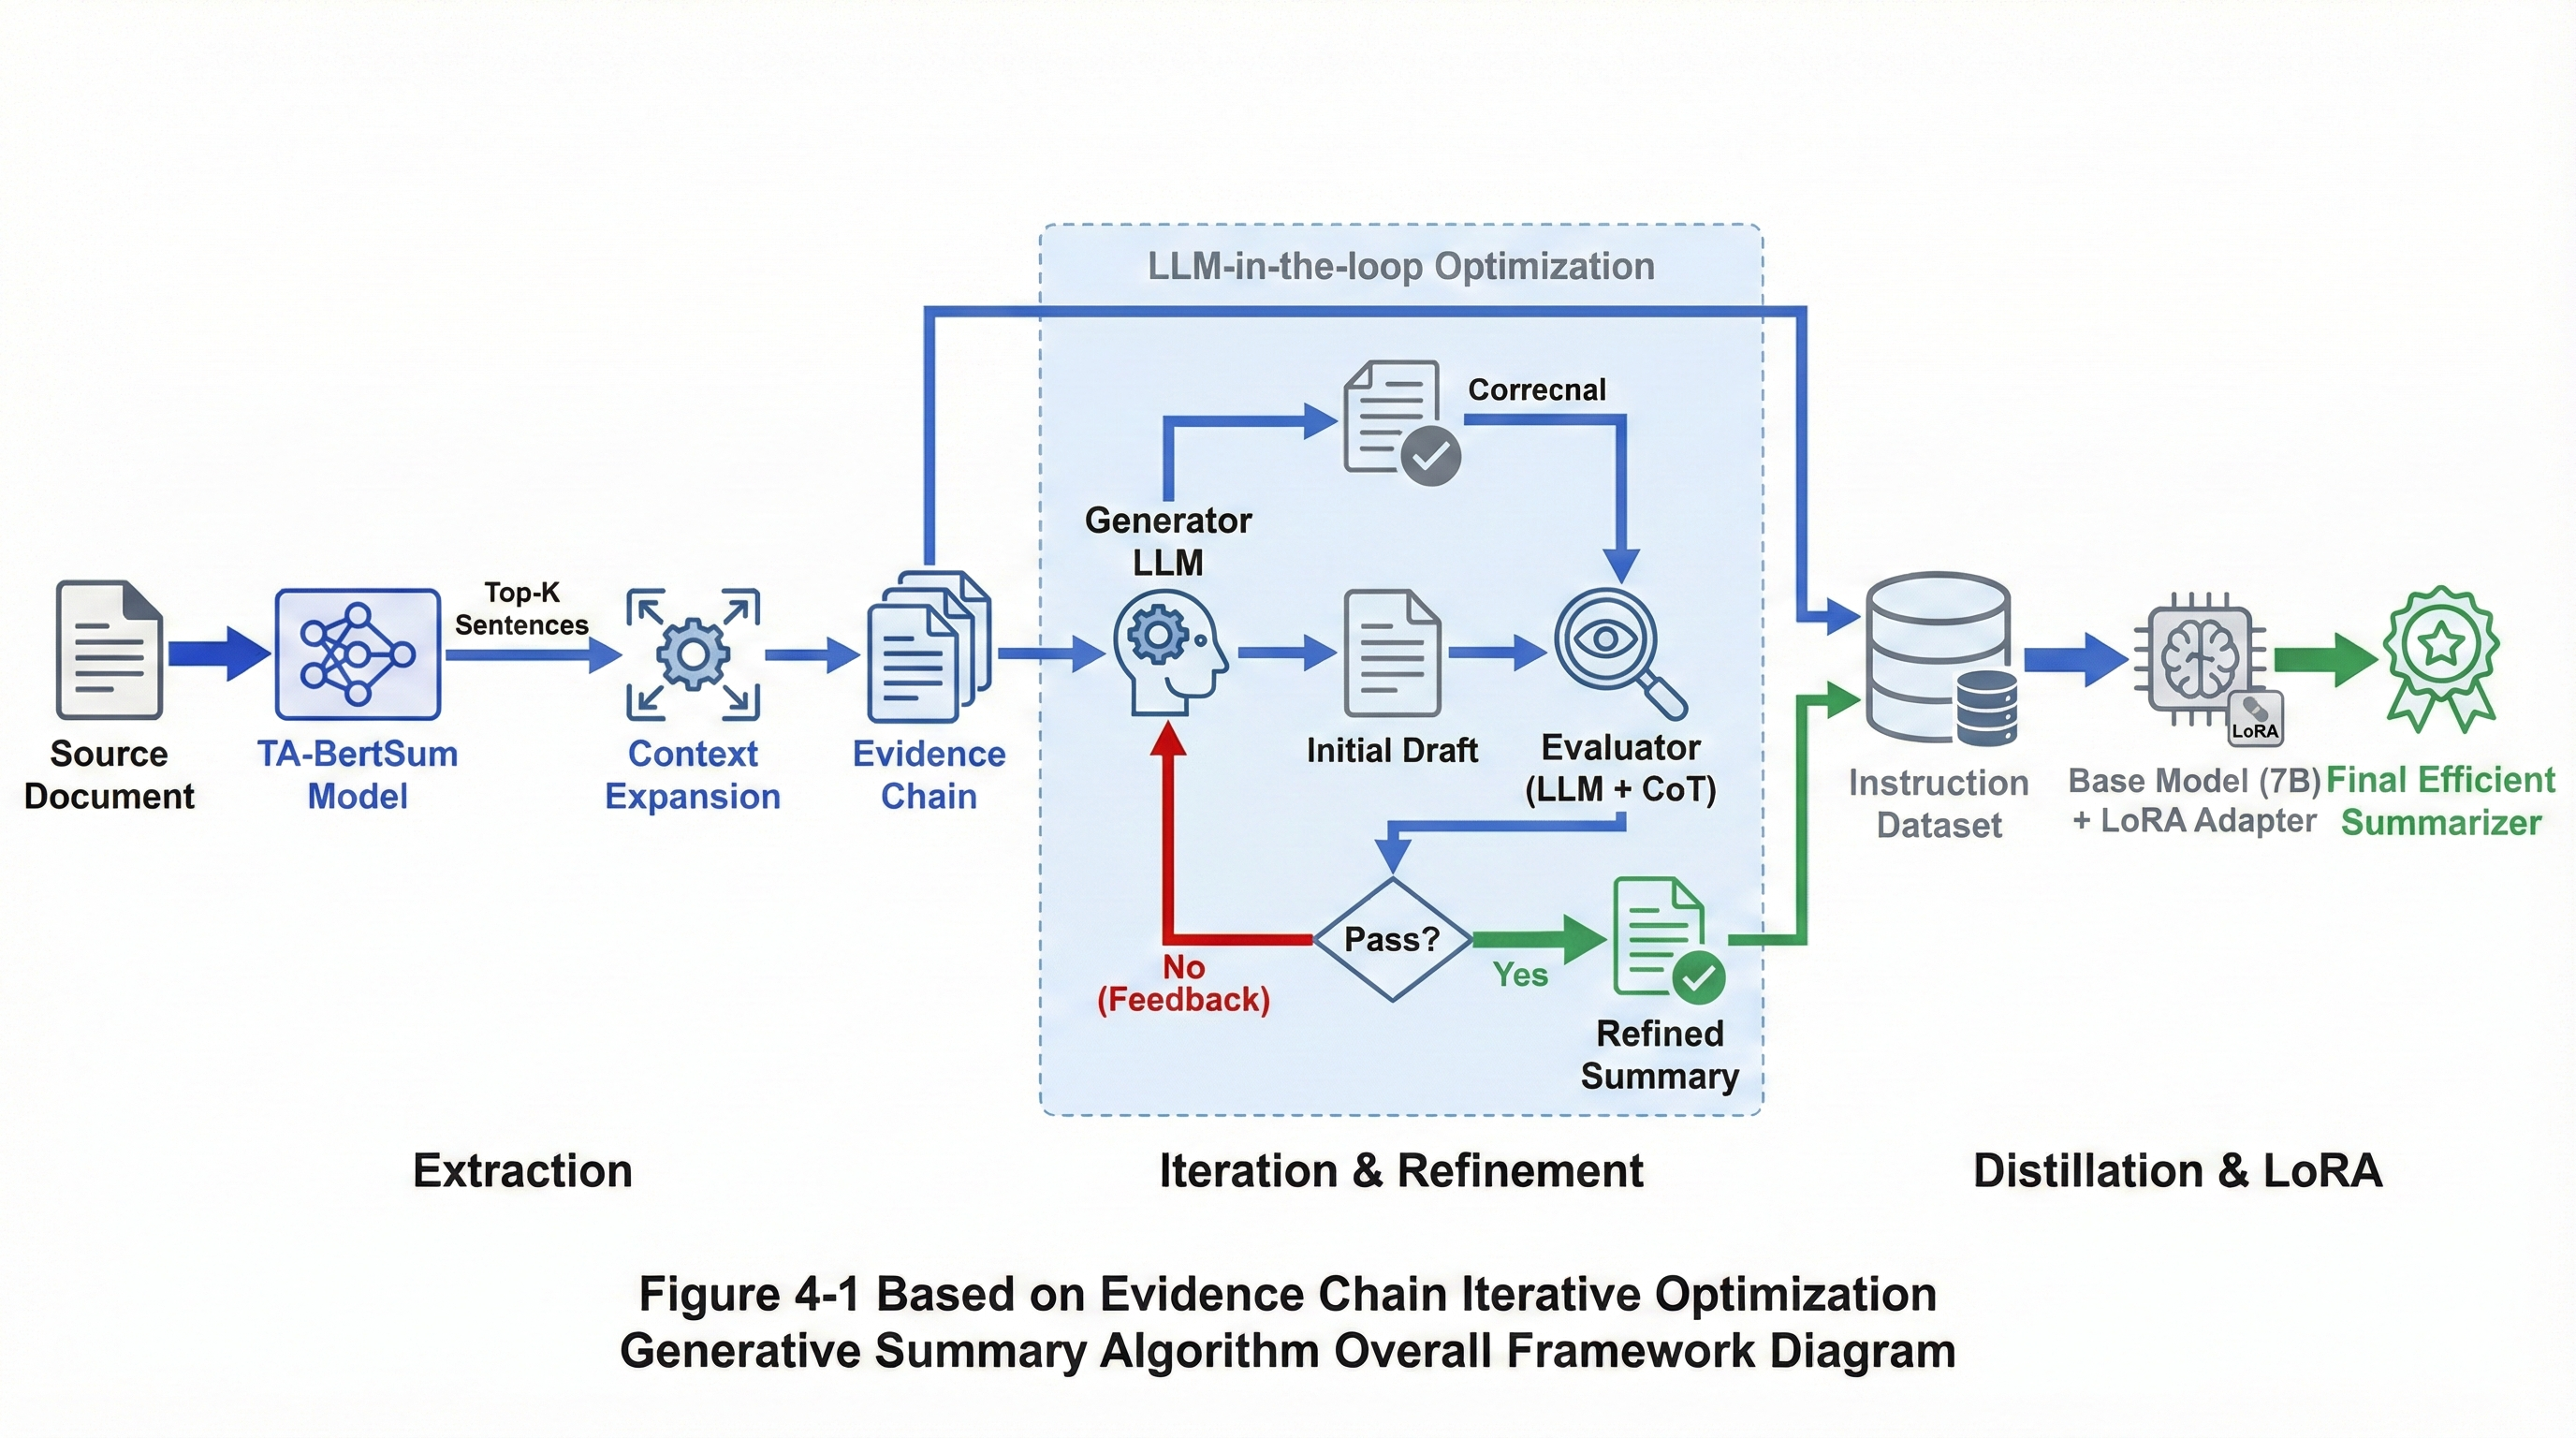
\includegraphics[trim={2cm 5cm 6cm 2cm}, clip,width=1\textwidth]{figure/chapter5/3.pdf} \caption{文档智能助手工作台:(a) 在线编辑与格式排版;(b) 智能摘要生成与多轮对话} \label{fig:showfirst2} \end{figure}
左侧编辑区旨在提供对标原生桌面级应用(如 Microsoft Word)的编辑体验。系统内置了高精度的文档解析引擎,能够完美处理从本地 Word(.docx)到云端 HTML 的跨格式转换;无论是复杂的嵌套表格、多层级列表,还是特殊的字体字号与段落间距,系统均能实现像素级还原,确保文档在跨平台流转过程中格式的高度一致性,有效解决了传统 Web 编辑器常见的样式丢失与错乱问题。在编辑功能上,系统具备全量的样式控制能力,功能覆盖率涵盖了文档处理的核心需求。用户不仅可以实时调整字体族、字号大小、文本颜色及背景高亮,还能通过可视化的交互方式处理单元格合并与拆分、边框样式调整等复杂表格操作,以及图片的缩放与混排。此外,通过对 DOM 树的实时操作与优化,系统实现了操作的毫秒级响应,配合内置的字数统计、撤销重做栈以及支持动态缩放的沉浸式阅读模式,为用户构建了一个流畅、专业且功能完备的云端写作环境。

右侧交互区集成了本文提出的智能体核心能力,实现了基于自然语言的文档处理自动化,交互区可以折叠或者展开,方便左侧的编辑区全屏阅读编辑。当用户在对话框输入指令时,前端并不直接请求大模型,而是先经过意图识别模块。若识别为生成摘要等指令,系统将自动触发 MCP 工具链;若识别为内容问答指令,则激活 RAG 检索流程。 如图 \ref{fig:showfirst2} (b) 所示,当触发摘要任务时,系统通过 MCP 协议调用底层算法提取关键信息,并结合 RAG 检索到的背景知识,构建结构化的 Prompt 上下文。生成的摘要并非静态文本,而是支持用户通过多轮对话进行渐进式修正。生成的结果按照文档内容的主题词、关键句、抽取式摘要和生成式摘要返回,同时得益于流式传输(Streaming)技术,大模型的生成结果能够通过流式传输实时返回,显著降低了用户的等待焦虑。 
\section{核心功能模块测试}
依据第三章的需求分析,本次测试重点关注文档格式处理和智能体摘要生成核心业务流程。

\paragraph{文档处理与格式转换测试}
该模块重点验证 Word 文档上传、HTML 高保真转换及在线编辑功能的稳定性。重点考察特殊格式如表格、目录在转换过程中的保留情况。测试用例及结果如表 \ref{tab:doc_test} 所示。

\begin{table}[H]
    \centering
    \caption{文档处理与格式转换功能测试用例}
    \label{tab:doc_test}
    % 使用 tabularx 自动换行,X 表示自适应宽度的列
    \begin{tabularx}{\textwidth}{c|l|X|c}
        \hline
        \textbf{编号} & \textbf{测试场景} & \textbf{测试步骤} & \textbf{结论} \\
        \hline
        TC-01 & 复杂格式的文档上传 & 上传包含目录、嵌套表格的 .docx 文档。系统成功解析,前端编辑器完整显示表格边框与目录层级。 & 通过 \\
        \hline
        TC-02 & 在线编辑与保存 & 修改文档内容并点击保存。后端将 HTML 转换为 .docx 流并存入文件系统,会生成新的文档。 & 通过 \\
        \hline
        TC-03 & 文档格式逆向导出 & 将在线编辑后的文档导出为本地文件。下载的 .docx 文件排版与在线编辑视图一致,无乱码。 & 通过 \\
        \hline
    \end{tabularx}
\end{table}

\paragraph{智能体摘要生成与 CoT 自修正测试}
此部分验证前述章节的提出的算法是否正确集成到系统,即基于 MCP 调用的 BertSum 主题提取与 CoT 驱动的摘要生成闭环。测试重点在于观察系统是否能正确识别意图触发自修正机制生成摘要。测试结果如表 \ref{tab:agent_test} 所示。

\begin{table}[H]
    \centering
    \caption{智能体摘要生成功能测试用例}
    \label{tab:agent_test}
    \begin{tabularx}{\textwidth}{c|l|X|c}
        \hline
        \textbf{编号} & \textbf{测试场景} & \textbf{测试步骤与预期结果} & \textbf{结论} \\
        \hline
        TC-04 & 发送摘要生成 & 意图识别后,通过MCP 调用相关服务,输出生成器的初始摘要、主题词、评估器的反馈过程和最终摘要,响应迅速。 & 通过 \\
        \hline
        TC-05 & 发送总结全文 & 意图识别后,通过MCP 调用相关服务,输出生成器的初始摘要、主题词、评估器的反馈过程和最终摘要,响应迅速& 通过 \\
        \hline
    \end{tabularx}
\end{table}



\section{本章小节}
本章详细阐述了基于大语言模型的抽取-生成式自动文本摘要系统的工程实现细节。

首先,介绍了系统的混合数据库存储方案,通过关系型数据库MySQL与 向量数据库Milvus 的协同工作,实现了对用户信息、文档元数据及高维语义向量的高效管理,为上层应用提供了稳固的数据支撑。其次,深入解析了系统的关键技术架构,重点展示了 RAG 知识检索流水线、基于 MCP 协议的异构模型集成机制以及 CoT 驱动的智能对话逻辑,从工程层面解决了大模型在长文档处理中面临的上下文限制与幻觉问题。

在具体实现层面,本章从核心类设计、关键业务时序逻辑以及前端交互界面三个维度进行了全方位展示。通过构建高内聚、低耦合的分层后端架构,系统成功实现了文档的高保真格式转换、主题词的提取以及抽取-生成二阶段摘要生成的完整业务闭环。最后,通过展示集成富文本在线编辑与智能对话助手的工作台界面,验证了系统在实际应用场景中的可用性与良好的用户体验。本章的系统实现将前文提出的理论模型转化为可运行的实体。

% \begin{figure}[htbp]
%     \centering 
%     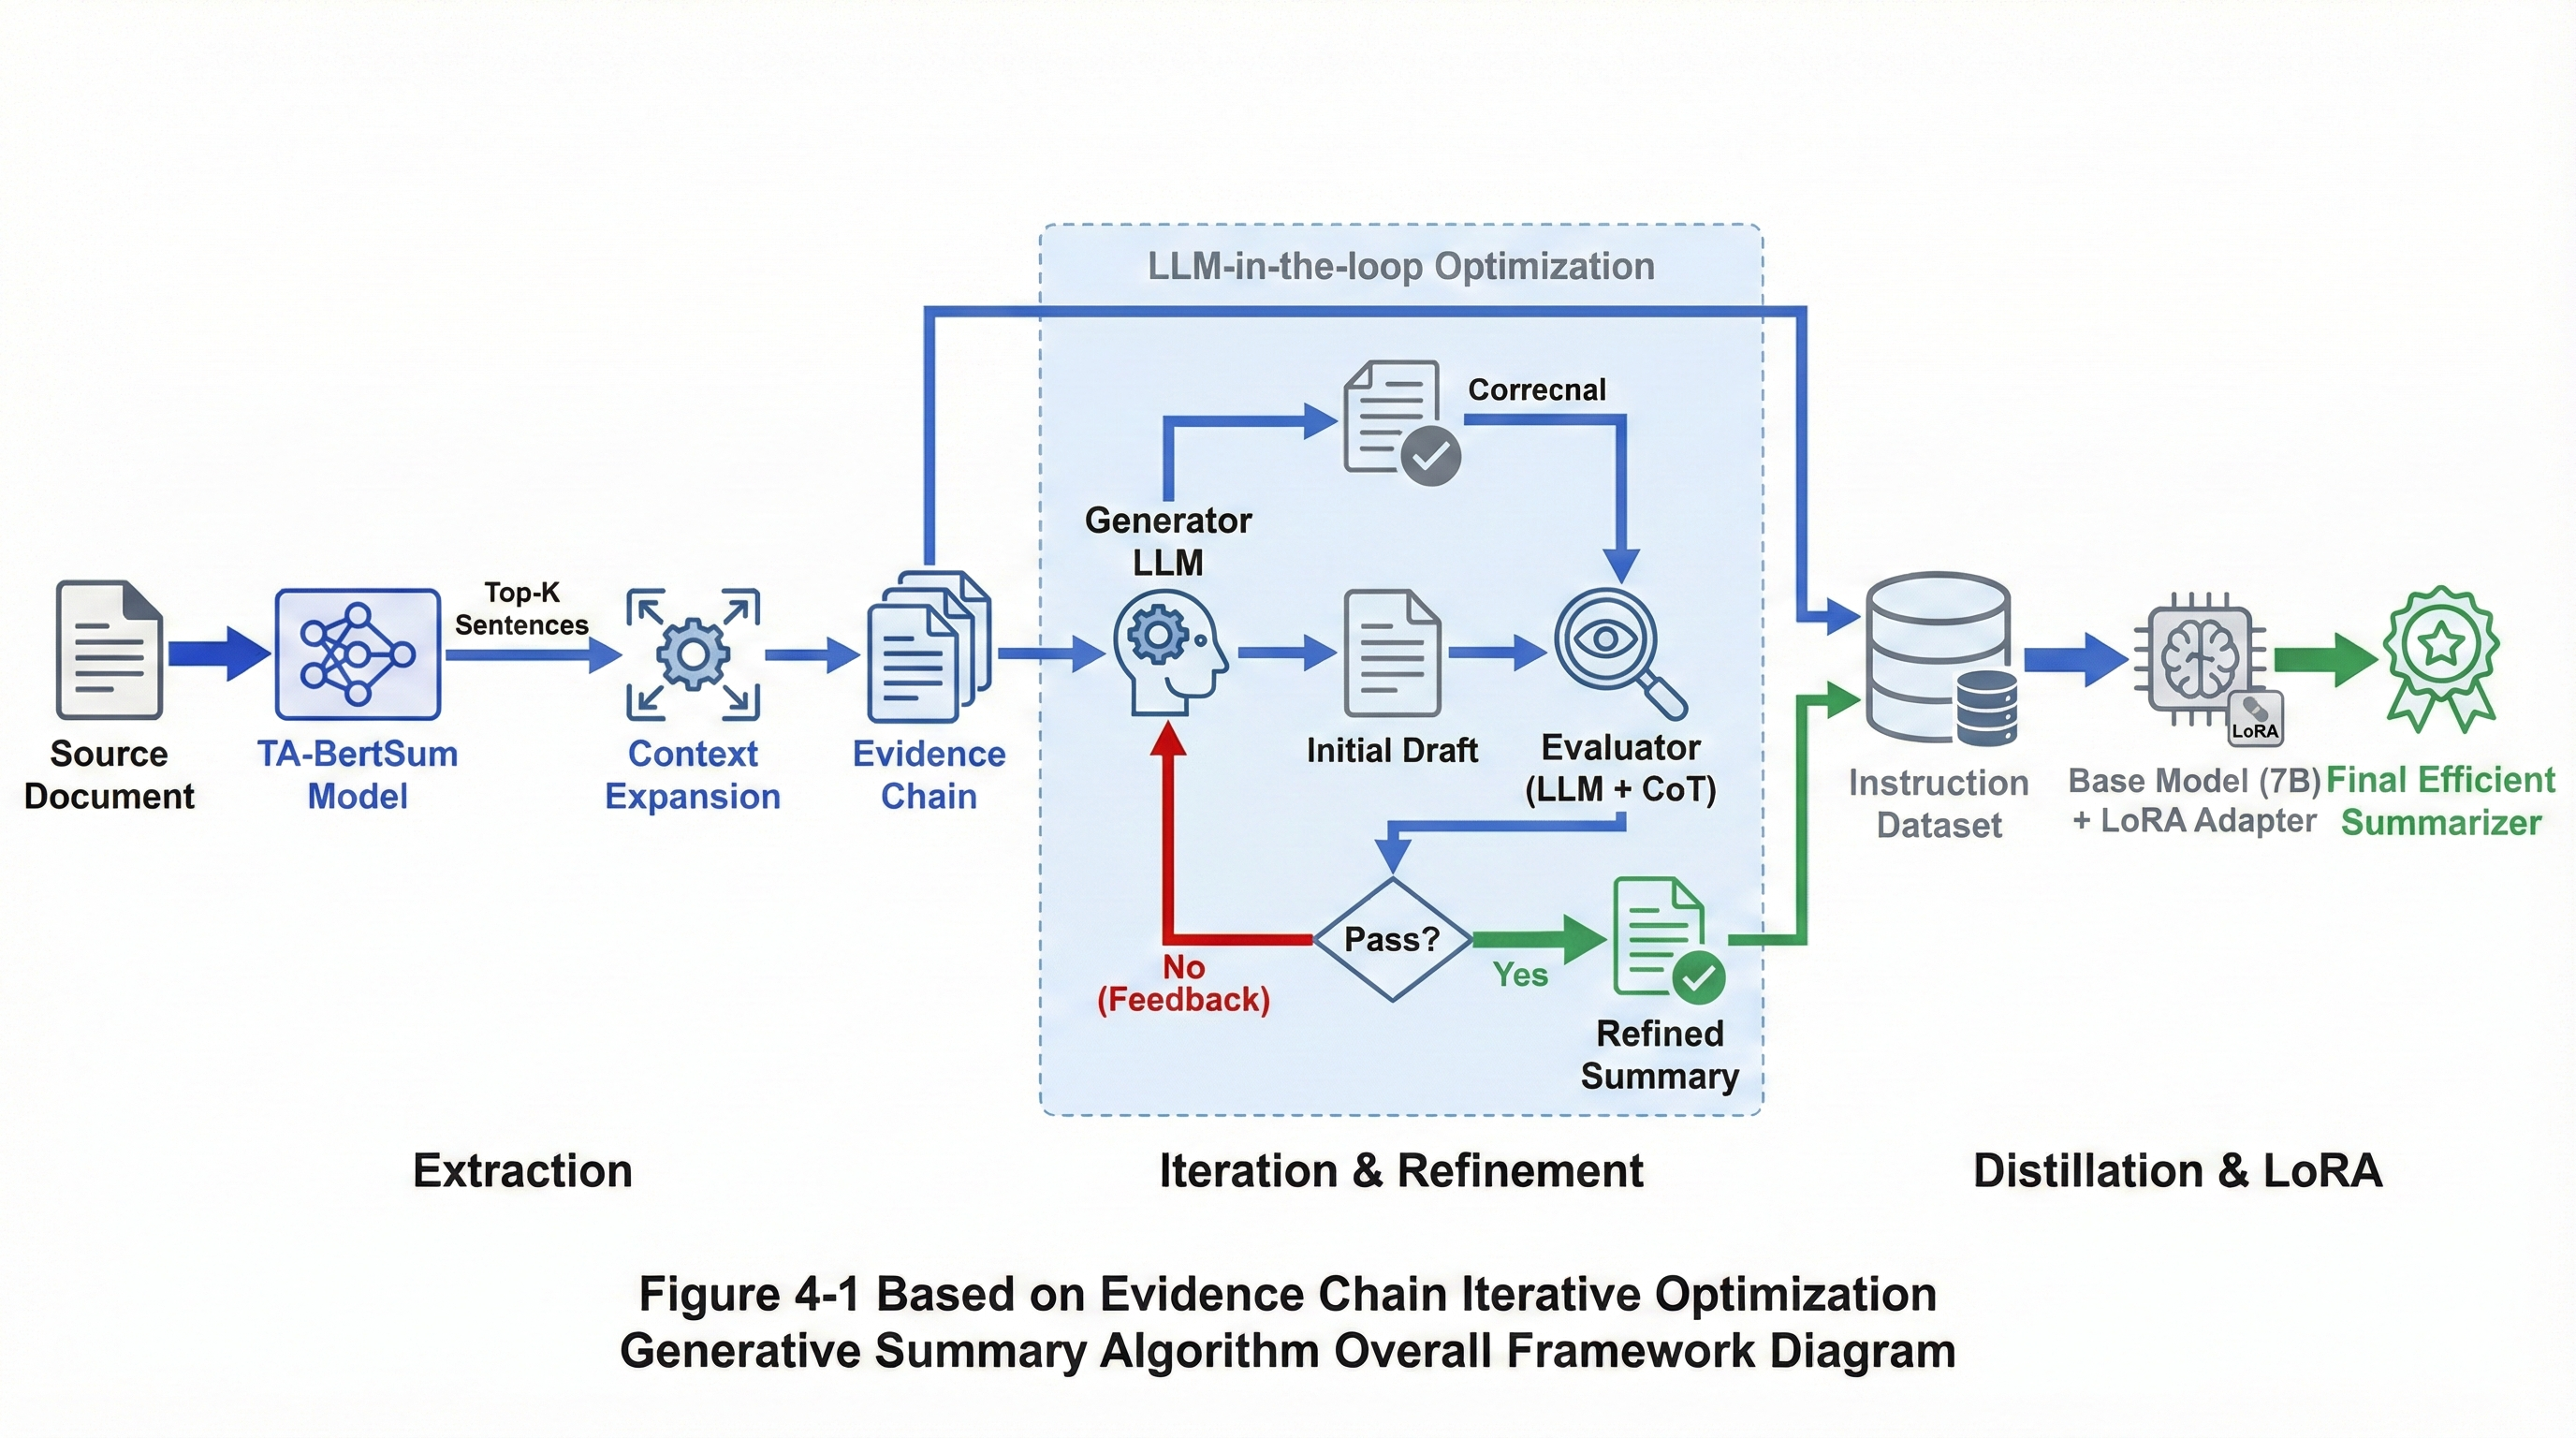
\includegraphics[trim={2cm 5cm 6cm 2cm}, clip,width=1\textwidth]{figure/chapter5/3.pdf}
%     \caption{系统页面截图2}
%     \label{fig:showfirst2}
% \end{figure}


% \subsection{}

%词云展示
%系统架构图
%各个接口的返回信息
%左下右上



\chapter{总结与展望}\section{工作总结}
本研究通过引入多粒度主题感知、证据链驱动迭代优化及智能体协同三大核心机制,显著提升了文档摘要的生成质量。具体贡献可归纳为以下三点:

\begin{enumerate}
    \item \textbf{提出基于多粒度主题感知的抽取式摘要模型}
    
    针对文档中关键信息分散与位置偏差问题,本文在第三章设计了TA-BertSum模型。该模型通过BERTopic挖掘文档的显式主题先验,设计主题偏置注意力机制,将全局主题信息以加性偏置形式注入自注意力层,重塑注意力分布以强化对长距离关键特征的捕捉。同时,设计全局门控融合模块,利用文档级主题向量对句子表征进行动态校准,缓解了预训练模型固有的Lead-3偏差。引入了主题语义对齐的对比损失函数。通过拉近摘要句与全局主题的距离并推离非摘要句,优化了特征空间的分布结构,显著提升了模型在 CNN/DailyMail、XSum 和 PubMed 等多领域数据集上的抽取性能 。
    
    \item \textbf{设计基于思维链的迭代优化生成式摘要框架}
    
    针对生成式模型的幻觉风险与逻辑混乱,第四章提出了证据链驱动的生成-评估-修正闭环框架。该框架首先利用TA-BertSum抽取的关键句构建高信噪比证据链,并通过局部上下文窗口增强算法修复语义碎片化。随后,引入基于CoT的迭代优化机制:生成器基于证据链生成初稿,评估器通过结构化提示工程对摘要进行多维审查,并增补、删除、重写等预定义指令。最终通过多轮迭代生成高质量摘要。此外,集成了反馈驱动的动态检索与FDR-SC算法,当检测到信息缺失时自动发起二次检索,确保知识补全的准确性。
    
    \item \textbf{实现基于智能体的文档摘要与编辑系统}
    
    为将理论研究转化为实用工具,第五章设计并开发了一款云端智能文档摘要生成和编辑系统。系统集成MCP协议与RAG技术,支持DOCX/PDF等格式的高保真转换与在线编辑。通过多智能体协同架构,实现了文档解析、摘要生成与交互式问答的全流程自动化。
\end{enumerate}

\section{研究展望}
尽管本文在长文档摘要生成领域取得了一定的研究成果,但受限于时间、算力及现有技术的局限性,仍存在一些不足之处,有待在未来的工作中进一步探索与完善:

\begin{enumerate}
    \item \textbf{提升迭代优化的推理效率}
    
    本文提出的生成-评估-修正框架虽然显著提升了摘要的忠实度与逻辑性,但多轮次的LLM推理与评估带来了较高的时间延迟。在处理超长文档或高并发请求时,系统的响应速度仍有待提升。未来的研究可以探索非自回归生成技术,或利用小模型蒸馏(Distillation)策略,将大模型的推理能力迁移至轻量级模型中,在保持生成质量的同时大幅降低推理成本与时间。
    
    \item \textbf{突破超长上下文的记忆瓶颈}
    
    虽然本文采用了证据链与RAG技术来缓解上下文限制,但在处理书籍级别或超长法律卷宗时,基于滑动窗口或分块处理的方法仍可能丢失跨段落的全局依赖。未来可尝试引入长上下文大模型或递归记忆网络机制,探索如何在无限上下文中保持对核心主旨的持续感知与精准回忆。
    
    \item \textbf{拓展多模态摘要生成能力}
    
    目前的文档摘要研究主要聚焦于纯文本内容。然而,在学术论文、行业研报等实际文档中,图表、公式与图片往往承载着关键信息。未来的工作可以尝试将多模态大模型引入摘要系统,实现图文并茂的多模态摘要生成(Multimodal Summarization),即在生成文本摘要的同时,自动选取或生成与内容匹配的关键图表,从而提供更直观、更全面的信息呈现方式。
\end{enumerate}
综上所述,尽管本文在文档摘要生成领域取得了一定的阶段性成果,验证了所提方法的有效性与鲁棒性,但受限于当前算力资源与模型机制的固有瓶颈,本研究在推理效率、超长上下文感知及多模态扩展等方面仍存在改进空间,有待在未来的工作中持续深耕。
\end{document}
